% Options for packages loaded elsewhere
\PassOptionsToPackage{unicode}{hyperref}
\PassOptionsToPackage{hyphens}{url}
%
\documentclass[
]{book}
\usepackage{amsmath,amssymb}
\usepackage{lmodern}
\usepackage{ifxetex,ifluatex}
\ifnum 0\ifxetex 1\fi\ifluatex 1\fi=0 % if pdftex
  \usepackage[T1]{fontenc}
  \usepackage[utf8]{inputenc}
  \usepackage{textcomp} % provide euro and other symbols
\else % if luatex or xetex
  \usepackage{unicode-math}
  \defaultfontfeatures{Scale=MatchLowercase}
  \defaultfontfeatures[\rmfamily]{Ligatures=TeX,Scale=1}
\fi
% Use upquote if available, for straight quotes in verbatim environments
\IfFileExists{upquote.sty}{\usepackage{upquote}}{}
\IfFileExists{microtype.sty}{% use microtype if available
  \usepackage[]{microtype}
  \UseMicrotypeSet[protrusion]{basicmath} % disable protrusion for tt fonts
}{}
\makeatletter
\@ifundefined{KOMAClassName}{% if non-KOMA class
  \IfFileExists{parskip.sty}{%
    \usepackage{parskip}
  }{% else
    \setlength{\parindent}{0pt}
    \setlength{\parskip}{6pt plus 2pt minus 1pt}}
}{% if KOMA class
  \KOMAoptions{parskip=half}}
\makeatother
\usepackage{xcolor}
\IfFileExists{xurl.sty}{\usepackage{xurl}}{} % add URL line breaks if available
\IfFileExists{bookmark.sty}{\usepackage{bookmark}}{\usepackage{hyperref}}
\hypersetup{
  pdftitle={Course Notes for Introduction to Statistics},
  pdfauthor={Dr.~Lauren Cappiello},
  hidelinks,
  pdfcreator={LaTeX via pandoc}}
\urlstyle{same} % disable monospaced font for URLs
\usepackage{color}
\usepackage{fancyvrb}
\newcommand{\VerbBar}{|}
\newcommand{\VERB}{\Verb[commandchars=\\\{\}]}
\DefineVerbatimEnvironment{Highlighting}{Verbatim}{commandchars=\\\{\}}
% Add ',fontsize=\small' for more characters per line
\usepackage{framed}
\definecolor{shadecolor}{RGB}{248,248,248}
\newenvironment{Shaded}{\begin{snugshade}}{\end{snugshade}}
\newcommand{\AlertTok}[1]{\textcolor[rgb]{0.94,0.16,0.16}{#1}}
\newcommand{\AnnotationTok}[1]{\textcolor[rgb]{0.56,0.35,0.01}{\textbf{\textit{#1}}}}
\newcommand{\AttributeTok}[1]{\textcolor[rgb]{0.77,0.63,0.00}{#1}}
\newcommand{\BaseNTok}[1]{\textcolor[rgb]{0.00,0.00,0.81}{#1}}
\newcommand{\BuiltInTok}[1]{#1}
\newcommand{\CharTok}[1]{\textcolor[rgb]{0.31,0.60,0.02}{#1}}
\newcommand{\CommentTok}[1]{\textcolor[rgb]{0.56,0.35,0.01}{\textit{#1}}}
\newcommand{\CommentVarTok}[1]{\textcolor[rgb]{0.56,0.35,0.01}{\textbf{\textit{#1}}}}
\newcommand{\ConstantTok}[1]{\textcolor[rgb]{0.00,0.00,0.00}{#1}}
\newcommand{\ControlFlowTok}[1]{\textcolor[rgb]{0.13,0.29,0.53}{\textbf{#1}}}
\newcommand{\DataTypeTok}[1]{\textcolor[rgb]{0.13,0.29,0.53}{#1}}
\newcommand{\DecValTok}[1]{\textcolor[rgb]{0.00,0.00,0.81}{#1}}
\newcommand{\DocumentationTok}[1]{\textcolor[rgb]{0.56,0.35,0.01}{\textbf{\textit{#1}}}}
\newcommand{\ErrorTok}[1]{\textcolor[rgb]{0.64,0.00,0.00}{\textbf{#1}}}
\newcommand{\ExtensionTok}[1]{#1}
\newcommand{\FloatTok}[1]{\textcolor[rgb]{0.00,0.00,0.81}{#1}}
\newcommand{\FunctionTok}[1]{\textcolor[rgb]{0.00,0.00,0.00}{#1}}
\newcommand{\ImportTok}[1]{#1}
\newcommand{\InformationTok}[1]{\textcolor[rgb]{0.56,0.35,0.01}{\textbf{\textit{#1}}}}
\newcommand{\KeywordTok}[1]{\textcolor[rgb]{0.13,0.29,0.53}{\textbf{#1}}}
\newcommand{\NormalTok}[1]{#1}
\newcommand{\OperatorTok}[1]{\textcolor[rgb]{0.81,0.36,0.00}{\textbf{#1}}}
\newcommand{\OtherTok}[1]{\textcolor[rgb]{0.56,0.35,0.01}{#1}}
\newcommand{\PreprocessorTok}[1]{\textcolor[rgb]{0.56,0.35,0.01}{\textit{#1}}}
\newcommand{\RegionMarkerTok}[1]{#1}
\newcommand{\SpecialCharTok}[1]{\textcolor[rgb]{0.00,0.00,0.00}{#1}}
\newcommand{\SpecialStringTok}[1]{\textcolor[rgb]{0.31,0.60,0.02}{#1}}
\newcommand{\StringTok}[1]{\textcolor[rgb]{0.31,0.60,0.02}{#1}}
\newcommand{\VariableTok}[1]{\textcolor[rgb]{0.00,0.00,0.00}{#1}}
\newcommand{\VerbatimStringTok}[1]{\textcolor[rgb]{0.31,0.60,0.02}{#1}}
\newcommand{\WarningTok}[1]{\textcolor[rgb]{0.56,0.35,0.01}{\textbf{\textit{#1}}}}
\usepackage{longtable,booktabs,array}
\usepackage{calc} % for calculating minipage widths
% Correct order of tables after \paragraph or \subparagraph
\usepackage{etoolbox}
\makeatletter
\patchcmd\longtable{\par}{\if@noskipsec\mbox{}\fi\par}{}{}
\makeatother
% Allow footnotes in longtable head/foot
\IfFileExists{footnotehyper.sty}{\usepackage{footnotehyper}}{\usepackage{footnote}}
\makesavenoteenv{longtable}
\usepackage{graphicx}
\makeatletter
\def\maxwidth{\ifdim\Gin@nat@width>\linewidth\linewidth\else\Gin@nat@width\fi}
\def\maxheight{\ifdim\Gin@nat@height>\textheight\textheight\else\Gin@nat@height\fi}
\makeatother
% Scale images if necessary, so that they will not overflow the page
% margins by default, and it is still possible to overwrite the defaults
% using explicit options in \includegraphics[width, height, ...]{}
\setkeys{Gin}{width=\maxwidth,height=\maxheight,keepaspectratio}
% Set default figure placement to htbp
\makeatletter
\def\fps@figure{htbp}
\makeatother
\setlength{\emergencystretch}{3em} % prevent overfull lines
\providecommand{\tightlist}{%
  \setlength{\itemsep}{0pt}\setlength{\parskip}{0pt}}
\setcounter{secnumdepth}{5}
\usepackage{booktabs}
\ifluatex
  \usepackage{selnolig}  % disable illegal ligatures
\fi
\usepackage[]{natbib}
\bibliographystyle{apalike}

\title{Course Notes for Introduction to Statistics}
\author{Dr.~Lauren Cappiello}
\date{}

\begin{document}
\maketitle

{
\setcounter{tocdepth}{1}
\tableofcontents
}
\hypertarget{introduction-to-data}{%
\chapter{Introduction to Data}\label{introduction-to-data}}

\hypertarget{module-overview}{%
\section{Module Overview}\label{module-overview}}

What is statistics? There are two ways to think about this:

\begin{enumerate}
\def\labelenumi{\arabic{enumi}.}
\tightlist
\item
  Facts and data, organized or summarized in such a way that they provide useful information about something.
\item
  The science of analyzing, organizing, and summarizing data.
\end{enumerate}

As a field, Statistics provides tools for scientists, practitioners, and laypeople to better understand data. You may find yourself using knowledge from this course in a research lab, while reading a research report, or even while watching the news!

\textbf{Module Learning Objectives/Outcomes}

After completing Module 1, you will:

\begin{enumerate}
\def\labelenumi{\arabic{enumi}.}
\tightlist
\item
  Understand basic statistical terminology.
\item
  Produce data using sampling and experimental design techniques.
\item
  Organize and visualize data using techniques for exploratory data analysis.
\item
  Identify the shape of a data set.
\item
  Understand and interpret graphical displays.
\end{enumerate}

This module's outcomes correspond to course outcomes (1) organize, summarize, and interpret data in tabular, graphical, and pictorial formats and (2) organize and interpret bivariate data and learn simple linear regression and correlation.

\hypertarget{statistics-terminology}{%
\section{Statistics Terminology}\label{statistics-terminology}}

There are two ways to think about statistics:

\begin{enumerate}
\def\labelenumi{\arabic{enumi}.}
\tightlist
\item
  \textbf{Descriptive statistics} are methods for \emph{describing} information.
\end{enumerate}

For example, 66\% of eligible voters voted in the 2020 presidential election (the highest turnout since 1900!).

\begin{enumerate}
\def\labelenumi{\arabic{enumi}.}
\setcounter{enumi}{1}
\tightlist
\item
  \textbf{Inferential statistics} are methods for \emph{drawing inference} (making decisions about something we are uncertain about).
\end{enumerate}

For example, a poll suggests that 75\% of voters will select a Candidate A. People haven't voted yet, so we don't know what will happen, but we could reasonably conclude that Candidate A will win the election.

\textbf{Data} is factual information. We collect data from a \textbf{population}, the collection of all individuals or items a researcher is interested in.

\begin{itemize}
\tightlist
\item
  Collecting data from an entire population is called a \textbf{census}.

  \begin{itemize}
  \tightlist
  \item
    This is complicated and expensive! There's a reason the United States only does a census every 10 years.
  \end{itemize}
\item
  We can also take a \textbf{sample}, a subset of the population we get data from.

  \begin{itemize}
  \tightlist
  \item
    If you think of the population as a pie, the sample is a small slice. If it's a good pie, the small slice will tell you that.
  \end{itemize}
\end{itemize}

\hypertarget{dig-deeper}{%
\subsection*{Dig Deeper}\label{dig-deeper}}
\addcontentsline{toc}{subsection}{Dig Deeper}

Read the article, \href{https://www.nytimes.com/2018/03/27/us/politics/census-citizenship-question.html}{Here's Why an Accurate Census Count Is So Important} from the New York Times. (If you can't access the article, try a Google search for ``why an accurate census count is important''.) Take a moment to write down your thoughts on the relationship between how we collect data (for example - the questions asked in the census) and the power data has over people's lives. As researchers, scientists, and consumers of media, what are some reasons this important to think about?

\hypertarget{data-basics}{%
\section{Data Basics}\label{data-basics}}

Data are often organized in what we call a \textbf{data matrix}. If you've ever seen data in a spreadsheet, that's a data matrix!

Age

Gender

Smoker

Marital Status

Person 1

45

Male

yes

married

Person 2

23

Female

no

single

Person 3

36

Other

no

married

Person 4

29

Female

no

single

Each row represents one \textbf{observation} (also called \textbf{observational units}, \textbf{cases}, or \textbf{subjects}). These are the individuals or items in the sample.

Each column represents a \textbf{variable}, the characteristic or thing being measured. Think of variables as measurements that can \emph{vary} from one observation to the next.

There are two types of variable:

\textbf{Numeric} or \textbf{quantitative} variables take \emph{numeric} values AND it is sensible to do math with those values.

\textbf{Discrete numeric} variables take numeric values with jumps. Typically, this means they can only take whole number values. A count of something is often discrete - counting the number of pets you have, for example.

\textbf{Continuous numeric} variables take values ``between the jumps''. Typically, this means they can take decimal values.

\textbf{Categorical} or \textbf{qualitative} variables take values that are \emph{categories}.

The ``Does it make sense''? test:

\begin{itemize}
\tightlist
\item
  Sometimes, categories can be represented by numbers. Ask yourself if it makes sense to do math with those numbers. If it doesn't make sense, it's probably a categorical variable. (Ex: zip codes)
\item
  If you're unsure whether a variable is discrete or continuous, pick a number with some decimal places - like 1.83 - and ask yourself if that value makes sense. If it doesn't, it's probably discrete. (Ex: number of siblings)
\end{itemize}

\hypertarget{sampling}{%
\section{Sampling}\label{sampling}}

How do we get samples? We want a sample that represents our population. \textbf{Representative samples} reflect the relevant characteristics of our population.

In general, we get representative samples by selecting our samples \emph{at random} and with an adequate sample size.

A non-representative sample is said to be \textbf{biased}. For example, if we used a sample of chihuahuas to represent all dogs, the sample would be biased.

These can be a result of \textbf{convenience sampling}, choosing a sample based on ease.

In our daily lives, common sources of biases are \textbf{anecdotal evidence} and \textbf{availability bias}. Anecdotal evidence is data based on personal experience or observation. Typically this consists of only one or two observations and is NOT representative of the population.

\begin{quote}
\emph{Example}: anecdotal evidence. A friend tells you their grandpa smoked a pack of cigarettes a day and lived to be 100. Does this mean that cigarettes will help you live to 100? no!
\end{quote}

Availability bias is your brain's tendency to think that examples of things that come readily to mind are more representative than is actually the case.

\begin{quote}
\emph{Example}: availability bias. Shark attacks. Shark attacks are actually extremely uncommon, but the media tends to report on extreme anecdotes, making us more prone to this kind of bias!
\end{quote}

We avoid bias by taking random samples. One type of random sample is a \textbf{simple random sample}. We can think of this as ``raffle sampling'', like drawing names out of a hat. Each case (or each possible sample) has an equal chance of being selected. Knowing that A is selected doesn't tell us anything about whether B is selected. Instead of drawing from a hat, we usually use a \textbf{random number generator} using a computer.

\hypertarget{experimental-design}{%
\section{Experimental Design}\label{experimental-design}}

When we do research, we have two options:

Conduct an \textbf{experiment}, where researchers assign treatments to cases.

\textbf{Treatments} are experimental conditions.

In an experiment, cases may also be called \textbf{experimental units} (items or individuals on which the experiment is performed).

Conduct an \textbf{observational study}, where no conditions are assigned. These are often done for ethical reasons, like examining the impacts of smoking cigarettes. Can you think of another example?

Experiments allow us to infer causation. Observational studies do not.

Experimental design principles:

\textbf{Control}: two or more treatments are compared.

\textbf{Randomization}: experimental units are assigned to treatment groups (usually and preferably at random).

\textbf{Replication}: a large enough sample size is used to test each treatment many times (on many different experimental units).

\textbf{Blocking}: if variables other than treatment are likely to have an impact on study outcome, we use blocks.

For example, I might separate patients in a medical study into ``high risk'' and ``low risk'' blocks. I would randomly assign all of the high risk patients to a treatment and then randomly assign all of the low risk patients to a treatment.

This helps ensure an even distribution of high/low risk patients in each treatment group.

An experiment without blocking has a completely randomized design; an experiment with blocking has a randomized block design.

In an experimental setting, we talk about

Response variable: the characteristic of the experimental outcome being measured or observed.

Factor: a variable whose impact on the response variable is of interest in the experiment.

Levels: the possible values of a factor.

Treatment:~each experimental condition (based on combinations of factor levels).

In human subjects research, we do a little extra work:

If subjects do not know what treatment group they are in, the study is called~blind.

We use a placebo (fake treatment) to achieve this.

If neither subject nor the researchers who interact with them know the treatment group, it is~double blind.

This helps avoid bias caused by placebo effect, doctor's expectations for outcome, etc.!

\hypertarget{frequency-distributions}{%
\section{Frequency Distributions}\label{frequency-distributions}}

\hypertarget{qualitative-variables}{%
\subsection{Qualitative Variables}\label{qualitative-variables}}

\textbf{Frequency} (\textbf{count}): the number of times a particular value occurs.

A \textbf{frequency distribution} lists each distinct value with its frequency.

\begin{longtable}[]{@{}cc@{}}
\toprule
Class & Frequency \\
\midrule
\endhead
freshman & 12 \\
sophomore & 10 \\
junior & 3 \\
senior & 5 \\
\bottomrule
\end{longtable}

A \textbf{bar plot} is a graphical representation of a frequency distribution. Each bar's height is based on the frequency of the corresponding category.

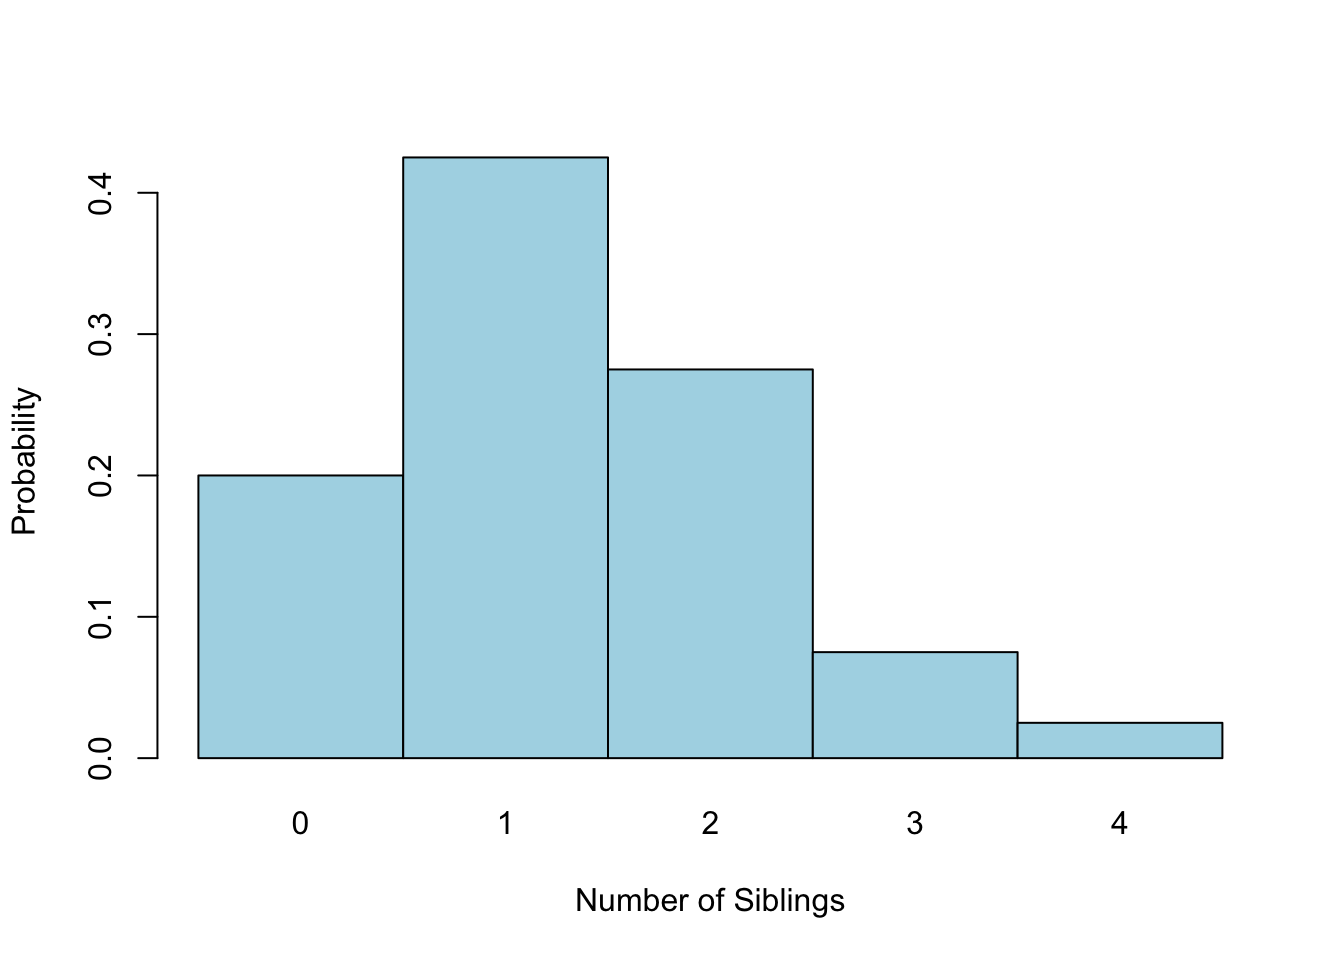
\includegraphics{IntroStats_files/figure-latex/unnamed-chunk-1-1.pdf}

The bar plot above shows the class level breakdown for students in an Introductory Statistics course. Take a moment to notice how the bars match up with the frequency distribution above.

\textbf{Relative frequency} is the ratio of the frequency to the total number of observations.

\[
  \text{relative frequency} = \frac{\text{frequency}}{\text{number of observations}}
\]

This is also called the \textbf{proportion}. The \textbf{percentage} can be obtained by multiplying the proportion by 100.

A \textbf{relative frequency distribution} lists each distinct value with its relative frequency.

\begin{longtable}[]{@{}ccc@{}}
\toprule
Class & Frequency & Relative Frequecy \\
\midrule
\endhead
freshman & 12 & \(12/30 = 0.4\) \\
sophomore & 10 & \(10/30 \approx 0.3333\) \\
junior & 3 & \(3/30 = 0.1\) \\
senior & 5 & \(5/30 \approx 0.1667\) \\
\bottomrule
\end{longtable}

\hypertarget{quantitative-variables}{%
\subsection{Quantitative Variables}\label{quantitative-variables}}

We can also apply this concept to numeric data. A \textbf{dot plot} is one graphical representation of this. A dot plot shows a number line with dots drawn above the line. Each dot represents a single point.

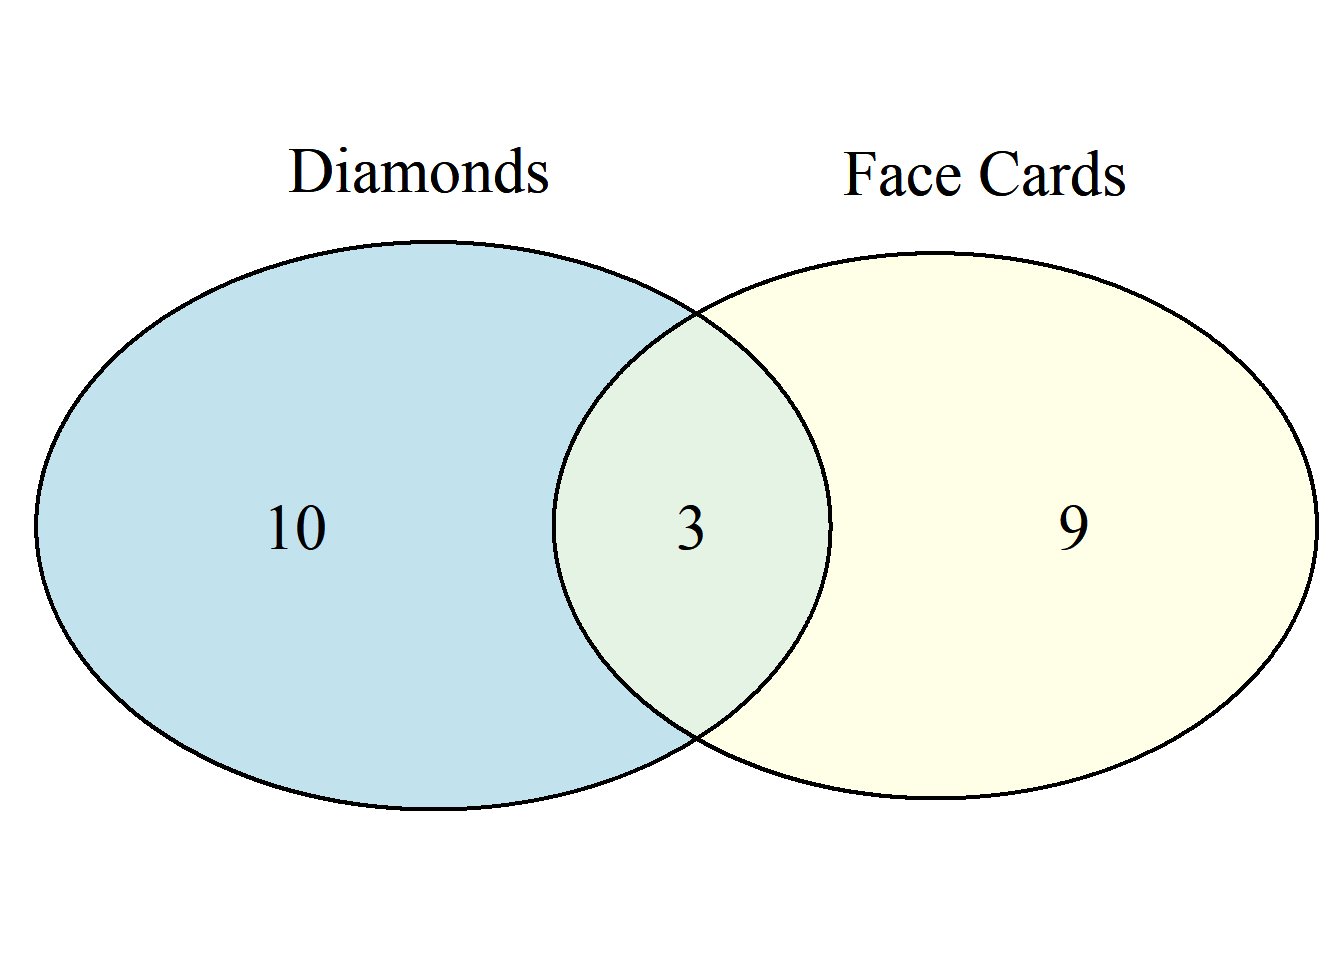
\includegraphics{IntroStats_files/figure-latex/unnamed-chunk-2-1.pdf}

For example, the dot plot above shows a sample where the number 1 appears 3 times, the number 5 appears 6 times, etc.

We would also like to be able to visualize larger, more complex data sets. We can do this using \textbf{bins}, which group numeric data into equal-width consecutive intervals.

\begin{quote}
\emph{Example}: A random sample of weights from 10 men, ages 18-24:

\[\quad 218.1 \quad 151.3 \quad 178.7 \quad 187.0 \quad   165.8 \quad 188.7 \quad 175.4 \quad 182.5 \quad 187.5 \quad 165.0\]

The \textbf{minimum} (smallest value) is 151.3 and the \textbf{maximum} (largest value) is 218.1. There are lots of ways to break these into ``bins'', but what about\ldots{}

\begin{itemize}
\tightlist
\item
  150 - 170
\item
  170 - 190
\item
  190 - 210
\item
  210 - 230
\end{itemize}

Each bin has an equal width of 20, but if someone a weight of 190, would I use the second or third bin?? We need there to be no overlap. Instead, we can use:

\begin{longtable}[]{@{}cc@{}}
\toprule
Weight & Count \\
\midrule
\endhead
150 - \textless170 & 3 \\
170 - \textless190 & 6 \\
190 - \textless210 & 0 \\
210 - \textless230 & 1 \\
\bottomrule
\end{longtable}
\end{quote}

We will visualize this using a \textbf{histogram}, which is a lot like a bar plot but for numeric data:

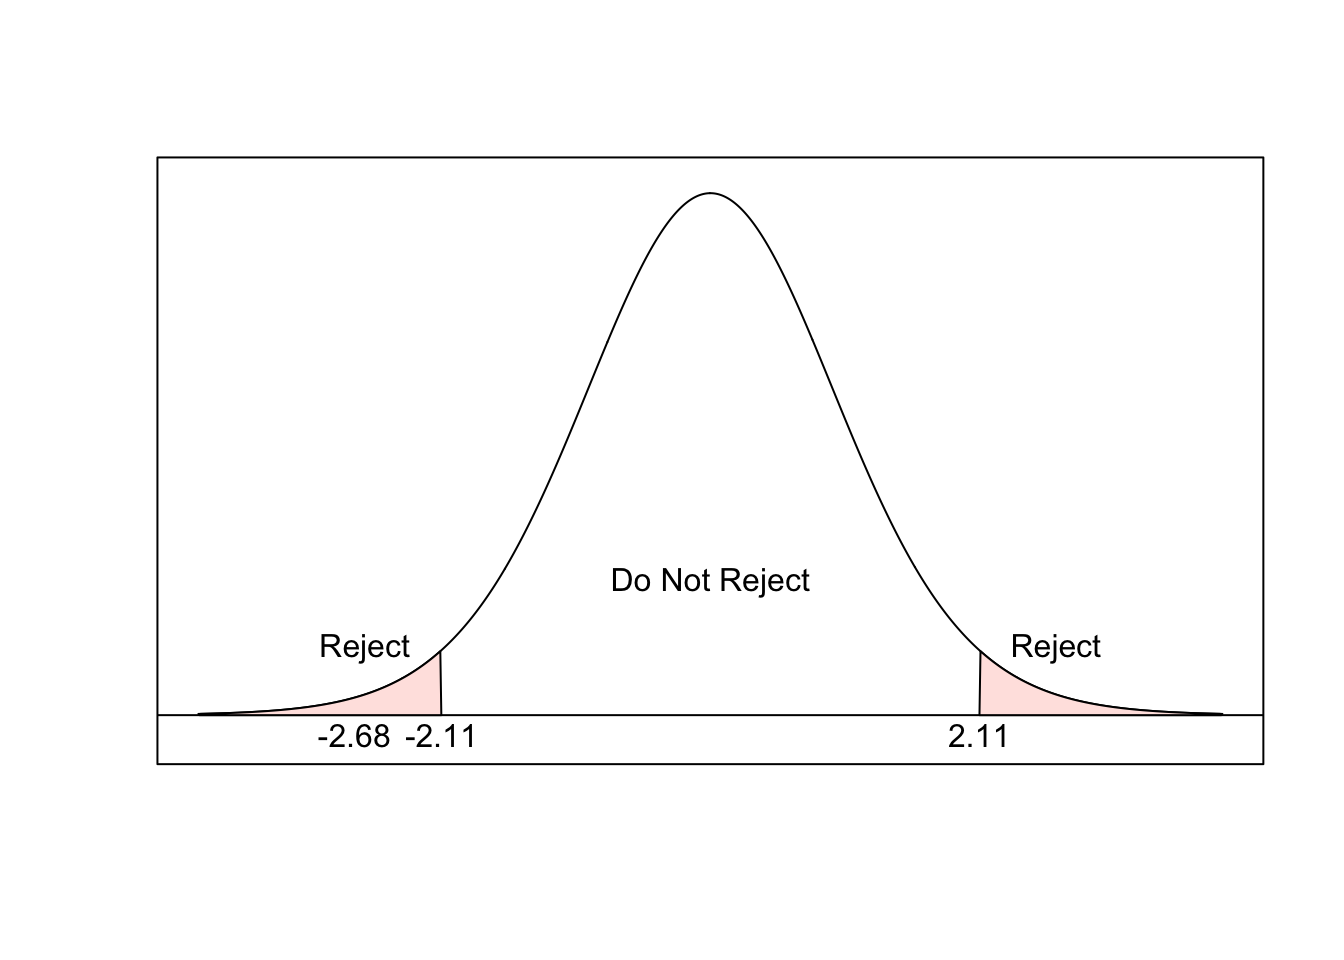
\includegraphics{IntroStats_files/figure-latex/unnamed-chunk-3-1.pdf}

This is what we call a \textbf{frequency histogram} because each bar height reflects the frequency of that bin. We can also create a \textbf{relative frequency histogram} which displays the relative frequency instead of the frequency:

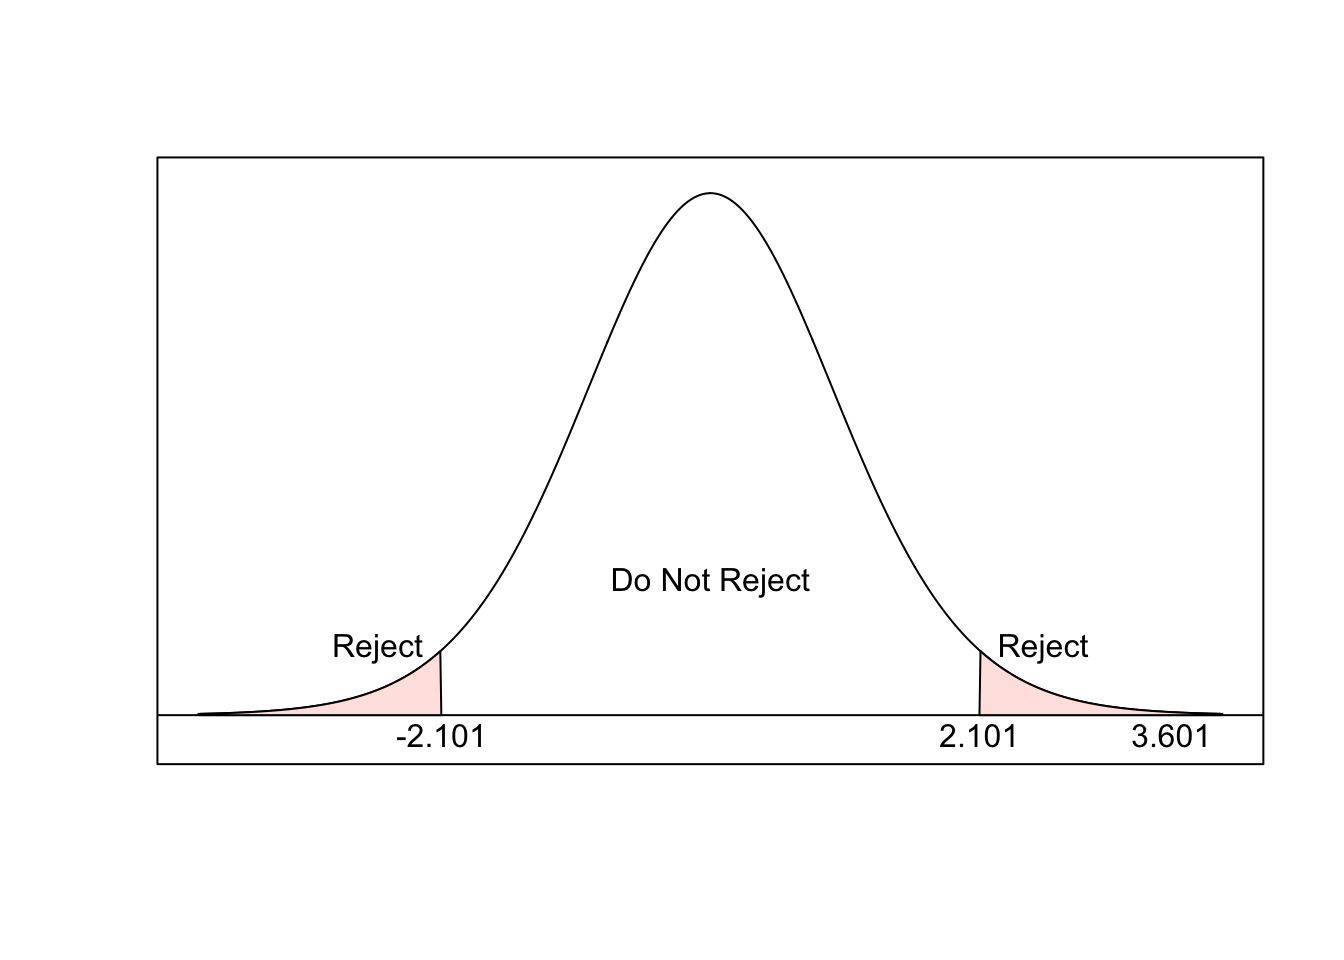
\includegraphics{IntroStats_files/figure-latex/unnamed-chunk-4-1.pdf}

Notice that these last two histograms look the same \emph{except for the numbers on the vertical axis}! This gives us insight into the shape of the data \textbf{distribution}, literally how the values are distributed across the bins. The part of the distribution that ``trails off'' to one or both sides is called a \textbf{tail} of the distribution.

When a histogram trails off to one side, we say it is \textbf{skewed} (right-skewed if it trails off to the right, left-skewed if it trails off to the left). Data sets with roughly equal tails are \textbf{symmetric}.

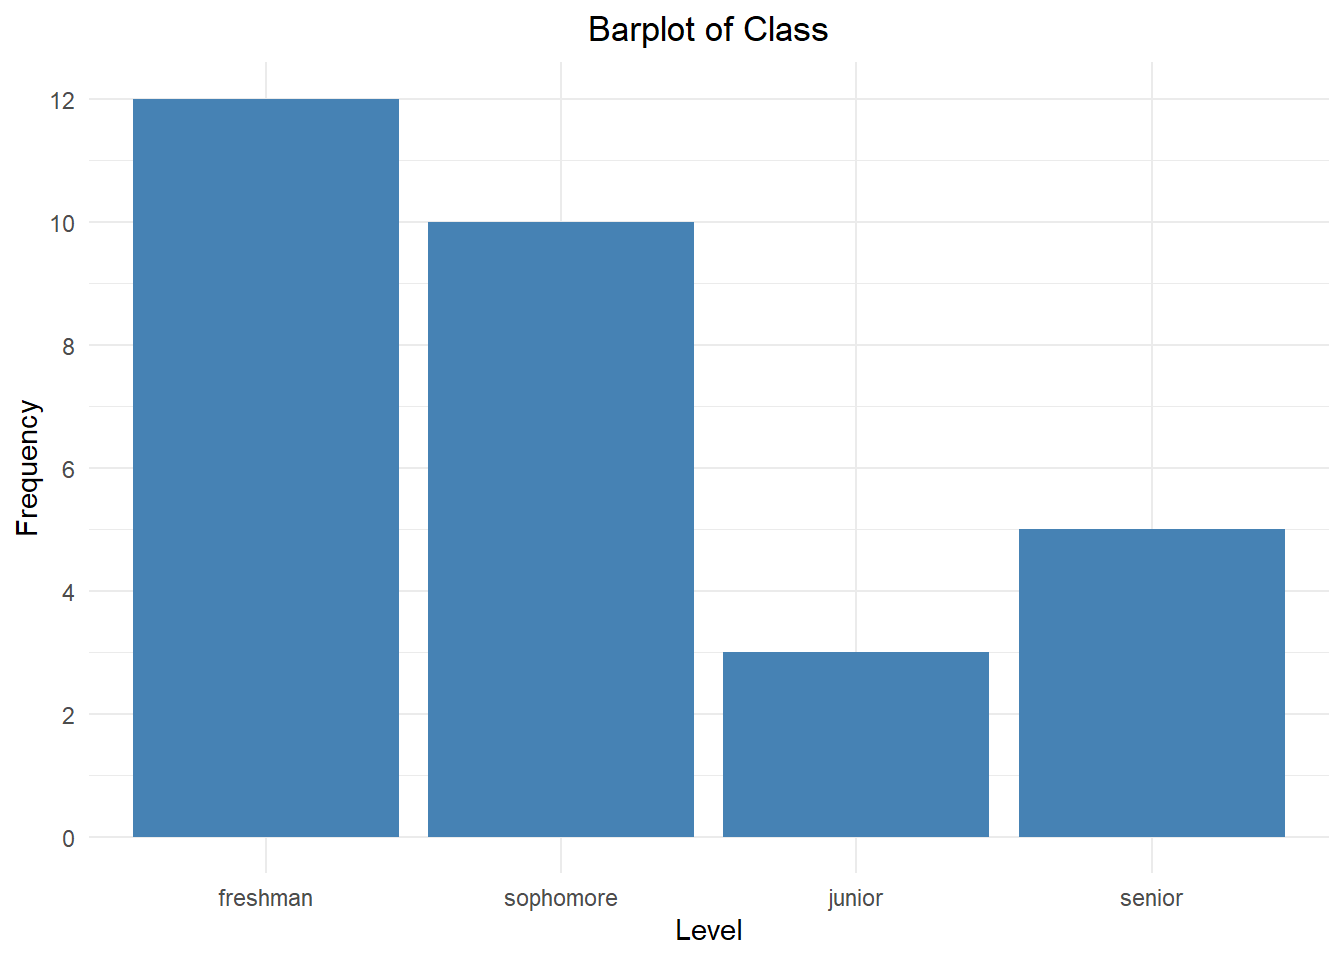
\includegraphics{IntroStats_files/figure-latex/unnamed-chunk-5-1.pdf}

We can also use a histogram to identify \textbf{modes}. For numeric data, especially continuous variables, we think of modes as \emph{prominent peaks}.

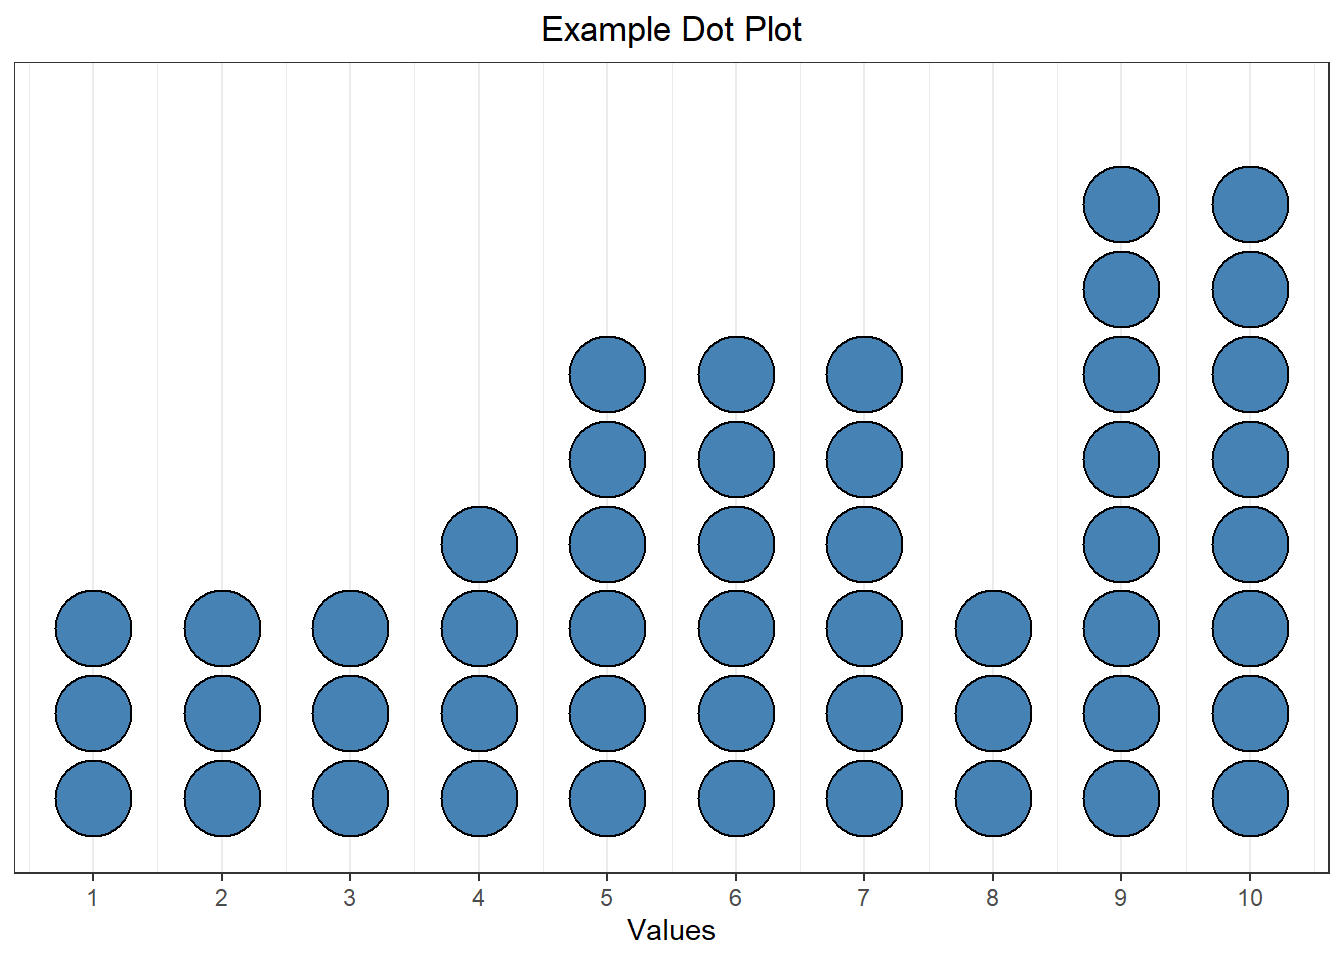
\includegraphics{IntroStats_files/figure-latex/unnamed-chunk-6-1.pdf}

\begin{itemize}
\tightlist
\item
  \textbf{Unimodal}: one prominent peak.
\item
  \textbf{Bimodal}: two prominent peaks.
\item
  \textbf{Multimodal}: three or more prominent peaks.
\end{itemize}

Finally, we can also ``smooth out'' these histograms and use a smooth curve to examine the shape of the distribution. Below are the smooth curve versions of the distributions shown in the four histograms used to demonstrate skew and symmetry.

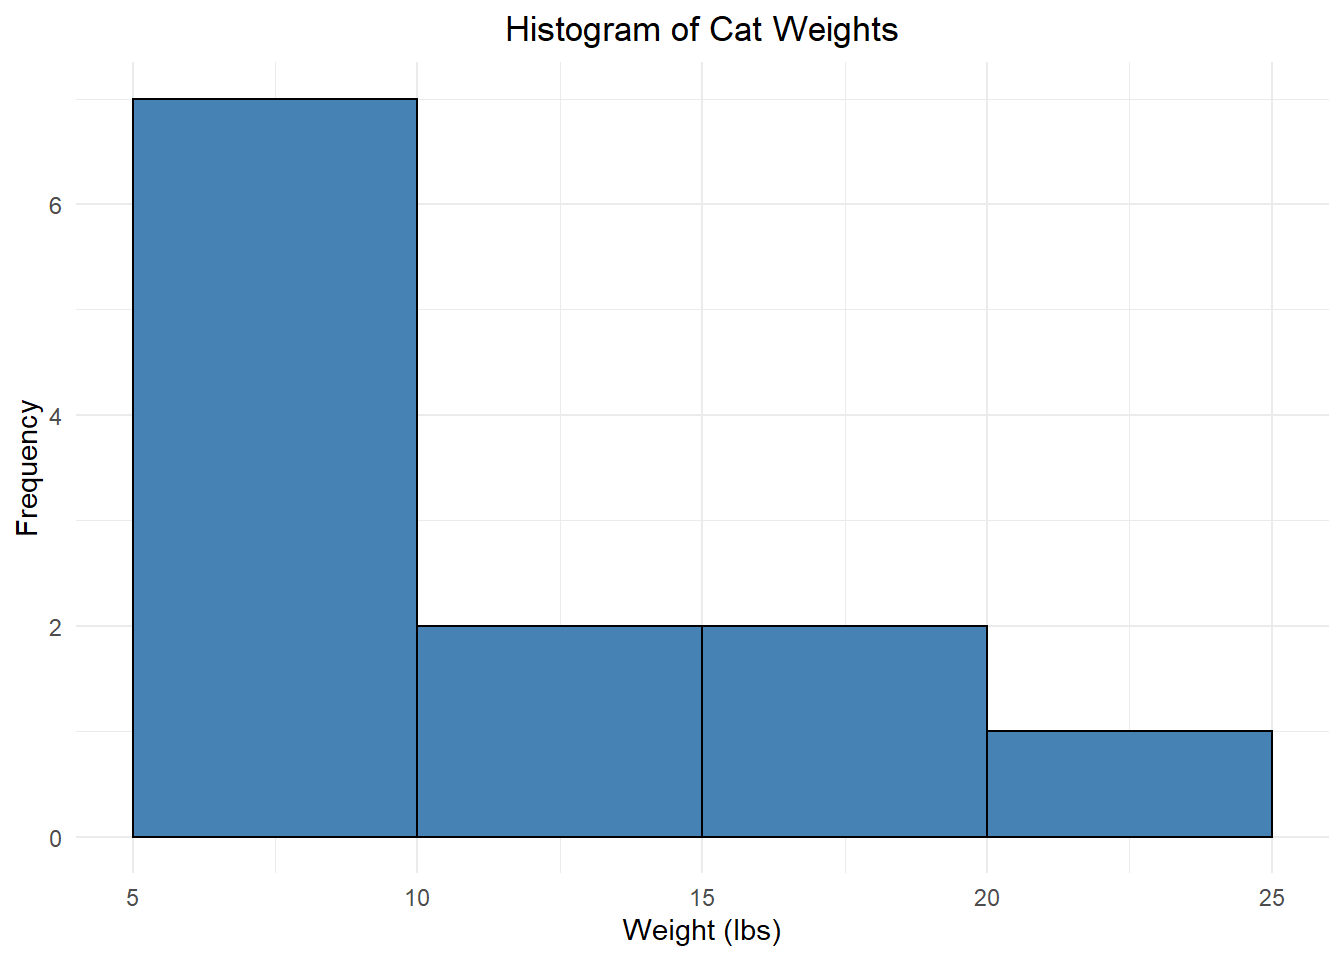
\includegraphics{IntroStats_files/figure-latex/unnamed-chunk-7-1.pdf}

\hypertarget{descriptive-measures}{%
\chapter{Descriptive Measures}\label{descriptive-measures}}

\hypertarget{module-overview-1}{%
\section{Module Overview}\label{module-overview-1}}

In the previous module, we thought about descriptive statistics using tables and graphs. Next, we summarize data by computing numbers. Some of these numbers you may already be familiar with, such as averages and percentiles. Numbers used to describe data are called descriptive measures. We also extend our conversation on descriptive measures for quantitative variables to include the relationship between two variables.

\textbf{Module Learning Objectives/Outcomes}

After completing Module 2, you will be able to:

\begin{enumerate}
\def\labelenumi{\arabic{enumi}.}
\tightlist
\item
  Calculate and interpret measures of center.
\item
  Calculate and interpret measures of variation.
\item
  Summarize data using boxplots.
\item
  Calculate and interpret a correlation coefficient.
\item
  Calculate and interpret a regression line.
\item
  Use a regression line to make predictions.
\end{enumerate}

This module's outcomes correspond to course outcomes (1) organize, summarize, and interpret data in tabular, graphical, and pictorial formats, (2) organize and interpret bivariate data and learn simple linear regression and correlation, and (6) apply statistical inference techniques of parameter estimation such as point estimation and confidence interval estimation.

\hypertarget{measures-of-central-tendency}{%
\section{Measures of Central Tendency}\label{measures-of-central-tendency}}

One research question we might ask is : what values are most common or most likely?

\textbf{Mode}: the most commonly occurring value.

\textbf{Mean}: this is what we usually think of as the ``average''. Denoted \(\bar{x}\). Add up all of the values and divide by the number of observations (\(n\)):
\[
  \bar{x} = \frac{x_1 + x_2 + \dots + x_n}{n} = \sum_{i=1}^n \frac{x_i}{n}
\]
where \(x_i\) denotes the \(i\)th observation and \(\sum_{i=1}^n\) is the sum of all observations from 1 through \(n\). This is called \emph{summation notation}.

\textbf{Median}: the middle number when the data are ordered from smallest to largest.

\begin{itemize}
\tightlist
\item
  If there are an odd number of observations, this will be the number in the middle:

  \{1, 3, \textbf{7}, 9, 9\} has median 7
\item
  If there are an even number of observations, there will be two numbers in the middle. The median will be their average.

  \{1, 2, \textbf{4, 7}, 9, 9\} has median \(\frac{4+7}{2}=5.5\)
\end{itemize}

The mean is sensitive to extreme values and skew. The median is not!

\(x\): 1, 3, 7, 9, 9

\(y\): 1, 3, 7, 9, 45

\(\bar{x} = \frac{29}{5} = 5.8\)

\(\bar{y} = \frac{65}{5} = 13\)

Notice how changing that 9 out for a 45 changes the \emph{mean} a lot! But the \emph{median} is 7 for both \(x\) and \(y\).

Because the median is not affected by extreme observations or skew, we say it is a \textbf{resistant measure} or that it is \textbf{robust}.

Which measure should we use?

\begin{itemize}
\tightlist
\item
  Mean: symmetric, numeric data
\item
  Median: skewed, numeric data
\item
  Mode: categorical data
\end{itemize}

Note: If the mean and median are roughly equal, it is reasonable to assume the distribution is roughly symmetric.

\hypertarget{measures-of-variability}{%
\section{Measures of Variability}\label{measures-of-variability}}

How much do the data vary?

Should we care? Yes! The more variable the data, the harder it is to be confident in our measures of center!

If you live in a place with extremely variable weather, it is going to be much harder to be confident in how to dress for tomorrow's weather\ldots{} but if you live in a place where the weather is always the same, it's much easier to be confident in what you plan to wear.

We want to think about how far observations are from the measure of center.

One easy way to think about variability is the \textbf{range} of the data: \[\text{range} = \text{maximum} - \text{minimum}\] This is quick and convenient, but it is \emph{extremely} sensitive to outliers! It also takes into account only two of the observations - we would prefer a measure of variaiblity that takes into account \emph{all} the observations.

\textbf{Deviation} is the distance of an observation from the mean: \(x - \bar{x}\). If we want to think about how far - on average - a typical observation is from the center, our intuition might be to take the average deviance\ldots{} but it turns out that summing up the deviances will \emph{always} result in 0! Conceptually, this is because the stuff below the mean (negative numbers) and the stuff above the mean (positive numbers) end up canceling each other out until we end up at 0.

One way to deal with this is to make all of the numbers positive, which we accomplish by squaring the deviance.

\begin{longtable}[]{@{}ccc@{}}
\toprule
& Deviance & Squared Deviance \\
\midrule
\endhead
\(x\) & \(x - \bar{x}\) & \((x - \bar{x})^2\) \\
2 & -1.2 & 1.44 \\
5 & 1.8 & 3.24 \\
3 & -0.2 & 0.04 \\
4 & 0.8 & 0.64 \\
2 & -1.2 & 1.44 \\
\(\bar{x}=3.2\) & Total = 0 & Total = 6.8 \\
\bottomrule
\end{longtable}

\textbf{Variance} (denoted \(s^2\)) is the average squared distance from the mean:
\[
  s^2 = \frac{(x_1-\bar{x})^2 + (x_2-\bar{x})^2 + \dots + (x_n-\bar{x})^2}{n-1} = \frac{1}{n-1}\sum_{i=1}^n (x_i - \bar{x})^2
\]
where \(n\) is the sample size. Notice that we divide by \(n-1\) and NOT by \(n\). There are some mathematical reasons why we do this, but the short version is that it'll be a better estimate when we move into Inference.

Finally, we come to \textbf{standard deviation} (denoted \(s\)). \[s = \sqrt{s^2}\] The standard deviation is the square root of the variance. We say that a ``typical" observation is about one standard deviation away from the mean.

We will think about one more measure of variability in the next section, the interquartile range.

\hypertarget{measures-of-position}{%
\section{Measures of Position}\label{measures-of-position}}

The \textbf{interquartile range} (\textbf{IQR}) represents the middle 50\% of the data.

Recall that the \emph{median} cut the data in half: 50\% of the data is below and 50\% is above the median. This is also called the \textbf{50th percentile}. The \textbf{\(p\)th percentile} is the value for which \(p\)\% of the data is below it.

To get the middle 50\%, we will split the data into four parts:

\begin{longtable}[]{@{}cccc@{}}
\toprule
1 & 2 & 3 & 4 \\
\midrule
\endhead
25\% & 25\% & 25\% & 25\% \\
\bottomrule
\end{longtable}

The 25th and 75th percentiles, along with the median, divide the data into four parts. We call these three measurements the \textbf{quartiles}:

\begin{itemize}
\tightlist
\item
  \textbf{Q1}, the first quartile, is the median of the lower 50\% of the data (the values below the median).
\item
  \textbf{Q2}, the second quartile, is the median.
\item
  \textbf{Q3}, the third quartile, is the median of the upper 50\% of the data (the values above the median).
\end{itemize}

\begin{quote}
\emph{Example}: Consider \{1, 2, 3, 4, 5, 6, 7, 8, 9, 10\}

\begin{itemize}
\tightlist
\item
  Cutting the data in half: \{1, 2, 3, 4, 5 \textbar{} 6, 7, 8, 9, 10\}, the median (Q2) is \(\frac{5+6}{2}=5.5\).
\item
  Q1 is the median of \{1, 2, 3, 4, 5\}, or 3
\item
  Q3 is the median of \{6, 7, 8, 9, 10\}, or 8
\end{itemize}
\end{quote}

Then the interquartile range is
\[
  \text{IQR} = \text{Q3}-\text{Q1}
\]

This is another measure of variability and is resistant to extreme values. In general, we prefer the mean and standard deviation when the data are symmetric and we prefer the median and IQR when the data are skewed.

\hypertarget{box-plots}{%
\subsection{Box Plots}\label{box-plots}}

Our measures of position are the foundation for constructing what we call a box plot, which summarizes the data with 5 statistics plus extreme observations:

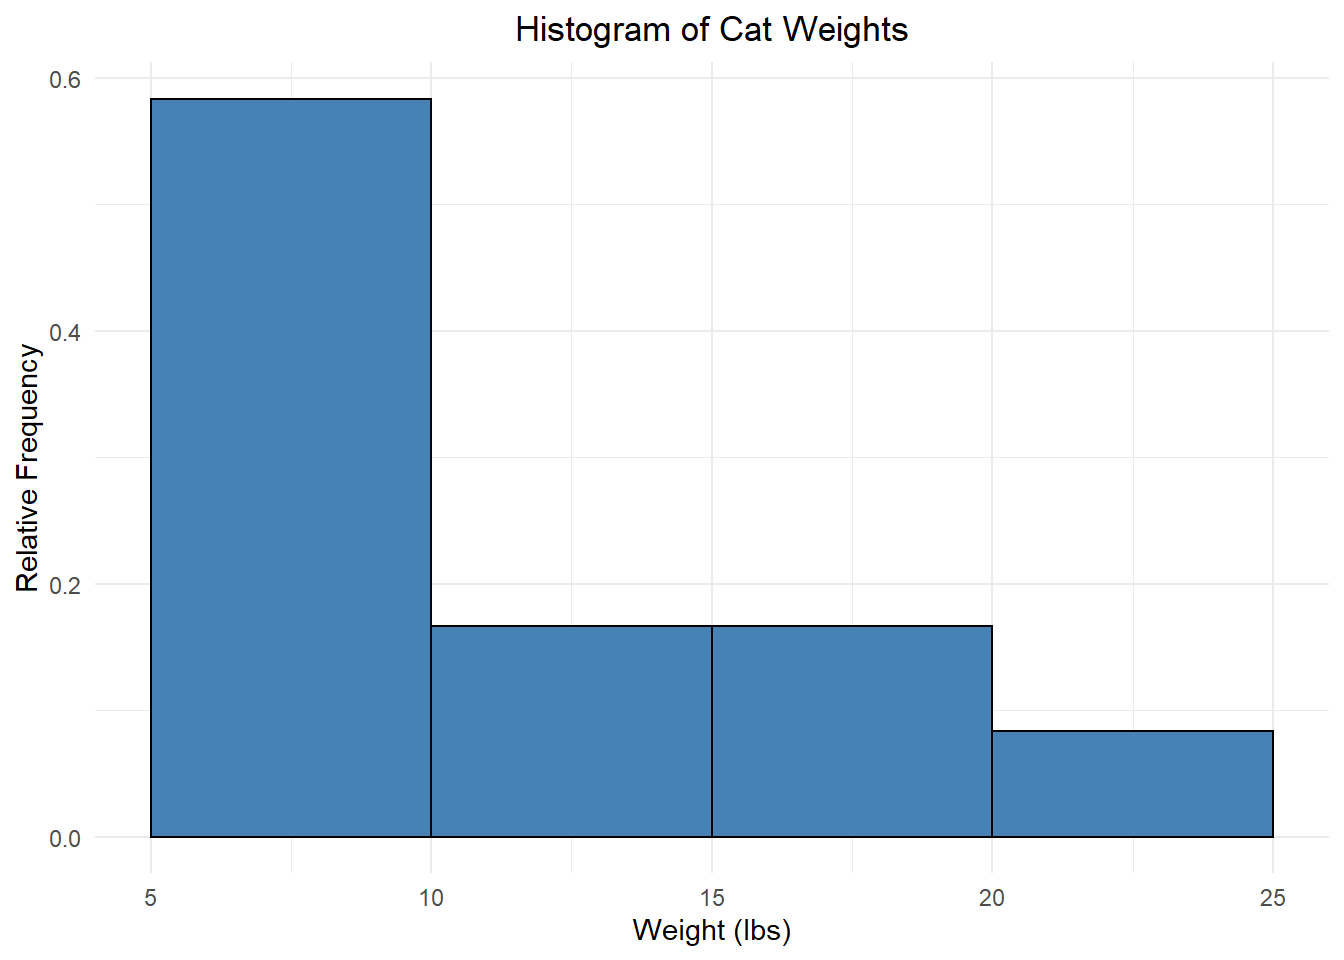
\includegraphics{IntroStats_files/figure-latex/unnamed-chunk-8-1.pdf}

Drawing a box plot:

\begin{enumerate}
\def\labelenumi{\arabic{enumi}.}
\tightlist
\item
  Draw the vertical axis to include all possible values in the data.
\item
  Draw a horizontal line at the median, at Q1, and at Q3. Use these to form a box.
\item
  Draw the \textbf{whiskers}. The whiskers' upper limit is Q3+1.5xIQR and the lower limit is Q1-1.5xIQR.
\item
  The actual whiskers are then drawn \emph{at the next closet point within the limit}.
\item
  Any points outside the whisker limits are included as individual points. These are \textbf{potential outliers}.
\end{enumerate}

(Potential) outliers can help us\ldots{}
- examine skew (outliers in the negative direction suggest left skew; outliers in the positive direction suggest right skew).
- identify issues with data collection or entry, especially if the value of the outliers doesn't make sense.

\hypertarget{descriptive-measures-for-populations}{%
\subsection{Descriptive Measures for Populations}\label{descriptive-measures-for-populations}}

So far, we've thought about calculating various descriptive statistics from a sample, but our long-term goal is to estimate descriptive information about a population. At the population level, these values are called \textbf{parameters}.

When we find a measure of center, spread, or position, we use a sample to calculate a single value. These single values are called \textbf{point estimates} and they are used to \emph{estimate} the corresponding population parameter. For example, we use \(\bar{x}\) to estimate the population mean, denoted \(\mu\) (Greek letter ``mu'') and \(s\) to estimate the population standard deviation, denoted \(\sigma\) (Greek letter ``sigma'').

\begin{longtable}[]{@{}ll@{}}
\toprule
Point Estimate & Parameter \\
\midrule
\endhead
sample mean: \(\bar{x}\) & population mean: \(\mu\) \\
sample standard deviation: \(s\) & population standard deviation: \(\sigma\) \\
\bottomrule
\end{longtable}

\ldots and so on and so forth. For each quantity we calculate from a sample (point estimate), there is some corresponding unknown population level value (parameter) that we wish to estimate.

We will discuss this in more detail when we discuss Random Variables and Statistical Inference.

\hypertarget{regression-and-correlation}{%
\section{Regression and Correlation}\label{regression-and-correlation}}

From your previous math classes, you should have a passing familiarity with linear equations like \(y=mx+b\). In statistics, we write these as \[y=b_0 + b_1x\] where \(b_0\) and \(b_1\) are constants, \(x\) is the independent variable, and \(y\) is the dependent variable. The graph of a linear function is always a (straight) line.

The \textbf{y-intercept} is \(b_0\), the value the dependent variable takes when the independent variable \(x=0\). The \textbf{slope} is \(b_1\), the change in \(y\) for a 1-unit change in \(x\).

A \textbf{scatterplot} shows the relationship between two (numeric) variables.

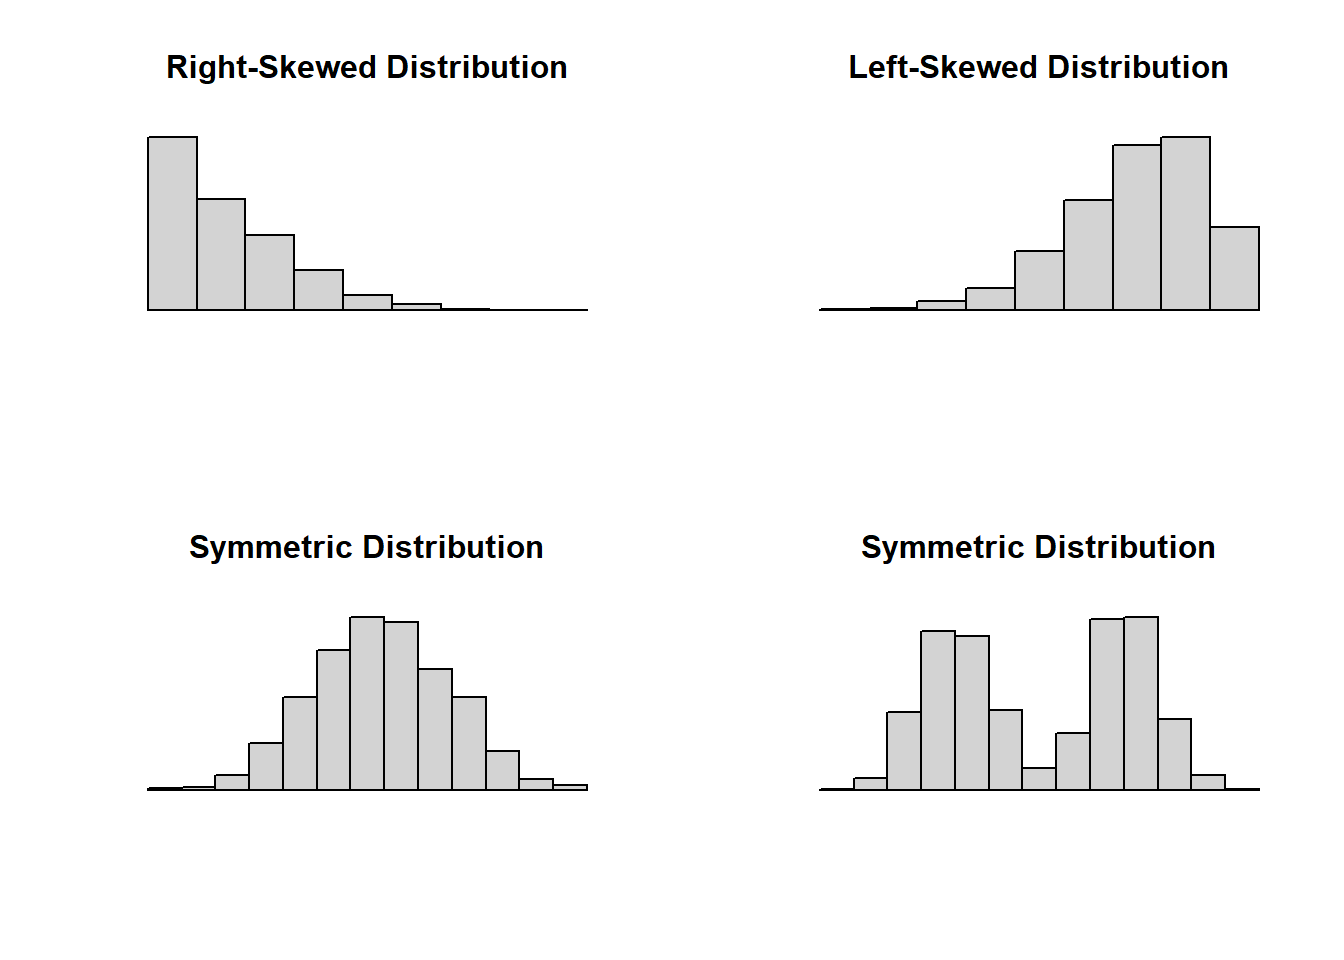
\includegraphics{IntroStats_files/figure-latex/unnamed-chunk-9-1.pdf}

At a glance, we can see that (in general) heavier cars have lower MPG. We call this type of data \textbf{bivariate data}. Now consider

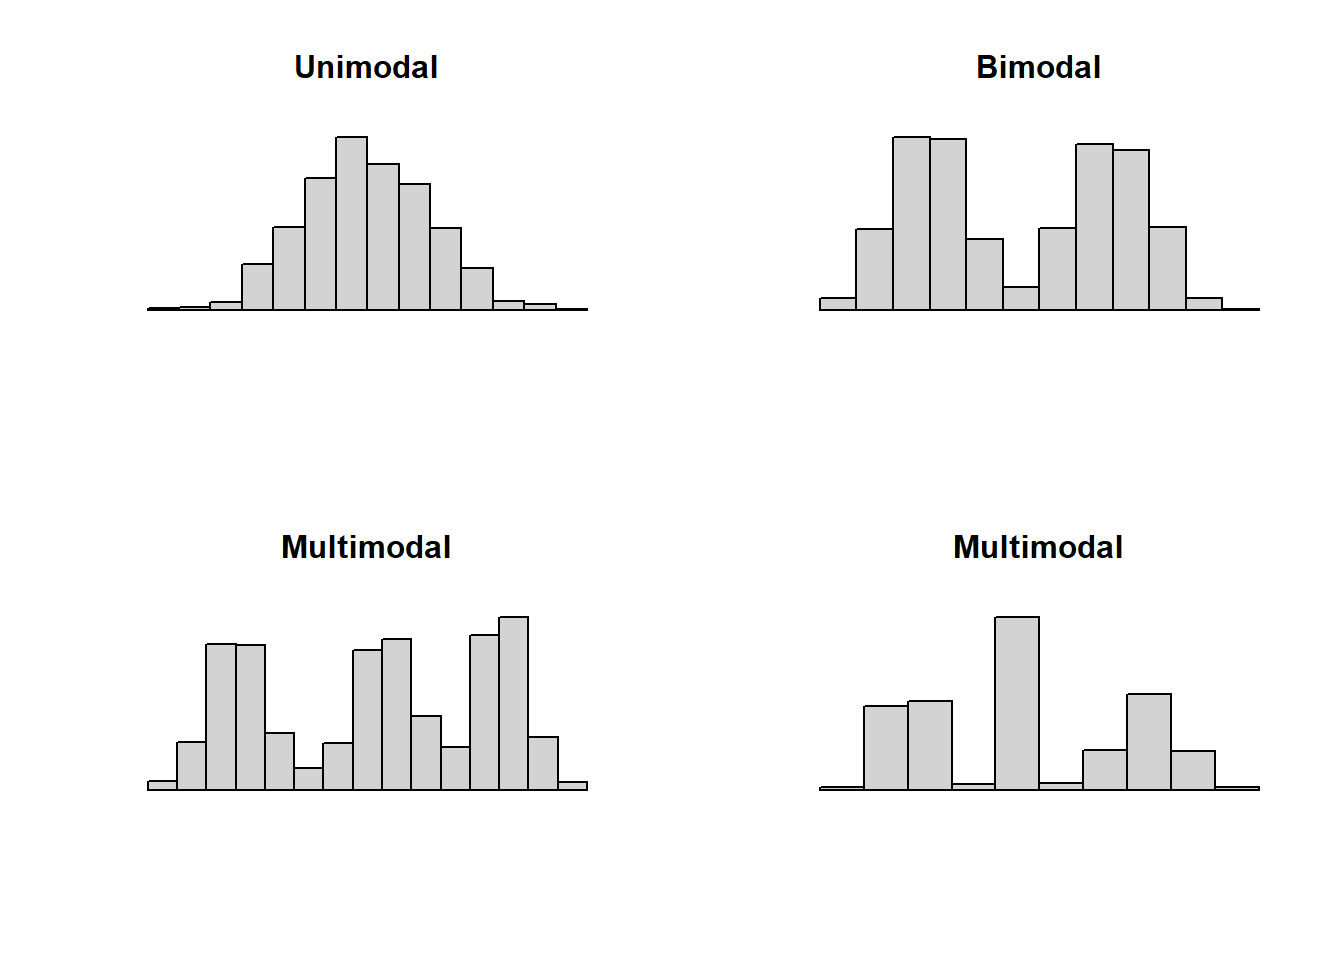
\includegraphics{IntroStats_files/figure-latex/unnamed-chunk-10-1.pdf}

This relationship can be modeled perfectly with a straight line:
\[
y = 8 + 3.25x
\]
When we can do this - model a relationship perfectly - we know the exact value of \(y\) whenever we know the value of \(x\). This is nice (we would love to be able to do this all the time!) but typically data is more complex than this.

Linear regression takes the idea of fitting a line and allows the relationship to be imperfect. Imagine in the previous scenario that you buy an \$8 pound of coffee each month and individual coffees cost \$3.25\ldots{} but what if your pound of coffee didn't always cost \$8? Or your coffee drinks didn't always cost \$3.25? In this case, you might get a plot that looks something like this:

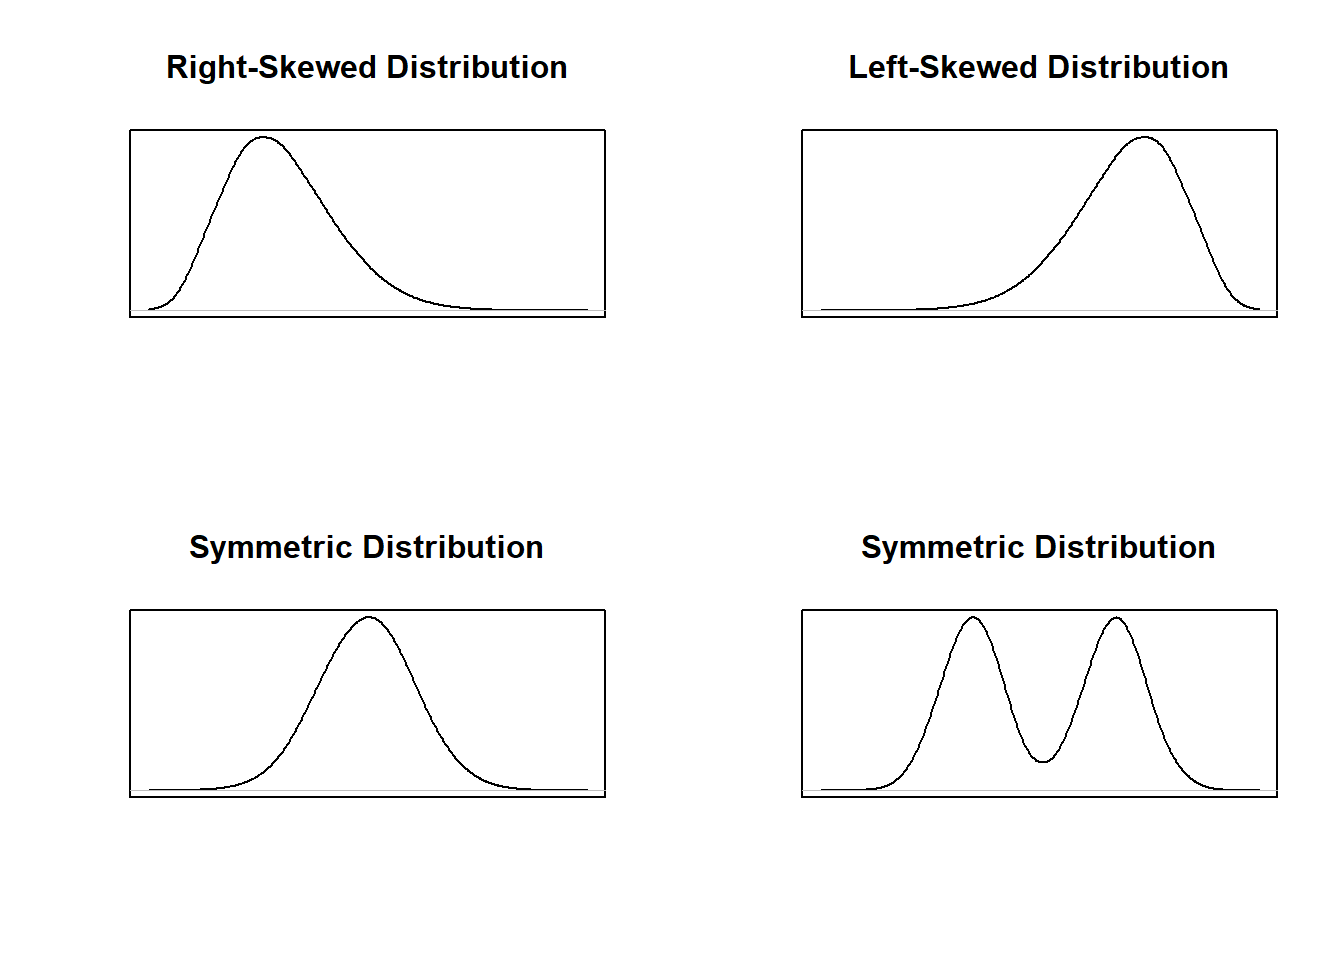
\includegraphics{IntroStats_files/figure-latex/unnamed-chunk-11-1.pdf}

The linear regression line looks like
\[
y = \beta_0 + \beta_1x + \epsilon
\]

\begin{itemize}
\tightlist
\item
  \(\beta\) is the Greek letter ``beta''.
\item
  \(\beta_0\) and \(\beta_1\) are constants.
\item
  Error (the fact that the points don't all line up perfectly) is represented by \(\epsilon\).
\end{itemize}

Think of this as the 2-dimensional version of a point estimate!

We estimate \(\beta_0\) and \(\beta_1\) using data and denote the estimated line by
\[
\hat{y} = b_0 + b_1x
\]

\begin{itemize}
\tightlist
\item
  \(\hat{y}\), ``y-hat'', is the estimated value of \(y\).
\item
  \(b_0\) is the estimate for \(\beta_0\).
\item
  \(b_1\) is the estimate for \(\beta_1\).
\end{itemize}

We drop the error term \(\epsilon\) when we estimate the constants for a regression line; we assume that the mean error is 0, so \emph{on average} we can ignore this error.

We use a regression line to make predictions about \(y\) using values of \(x\).

\begin{itemize}
\tightlist
\item
  \(y\) is the \textbf{response variable}.
\item
  \(x\) is the \textbf{predictor variable}.
\end{itemize}

\begin{quote}
\emph{Example}: (from OpenIntro Statistics 8.1.2) Researchers captured 104 brushtail possums and took a variety of body measurements on each before releasing them back into the wild. We consider two measurements for each possum: total body length and head length.
\end{quote}

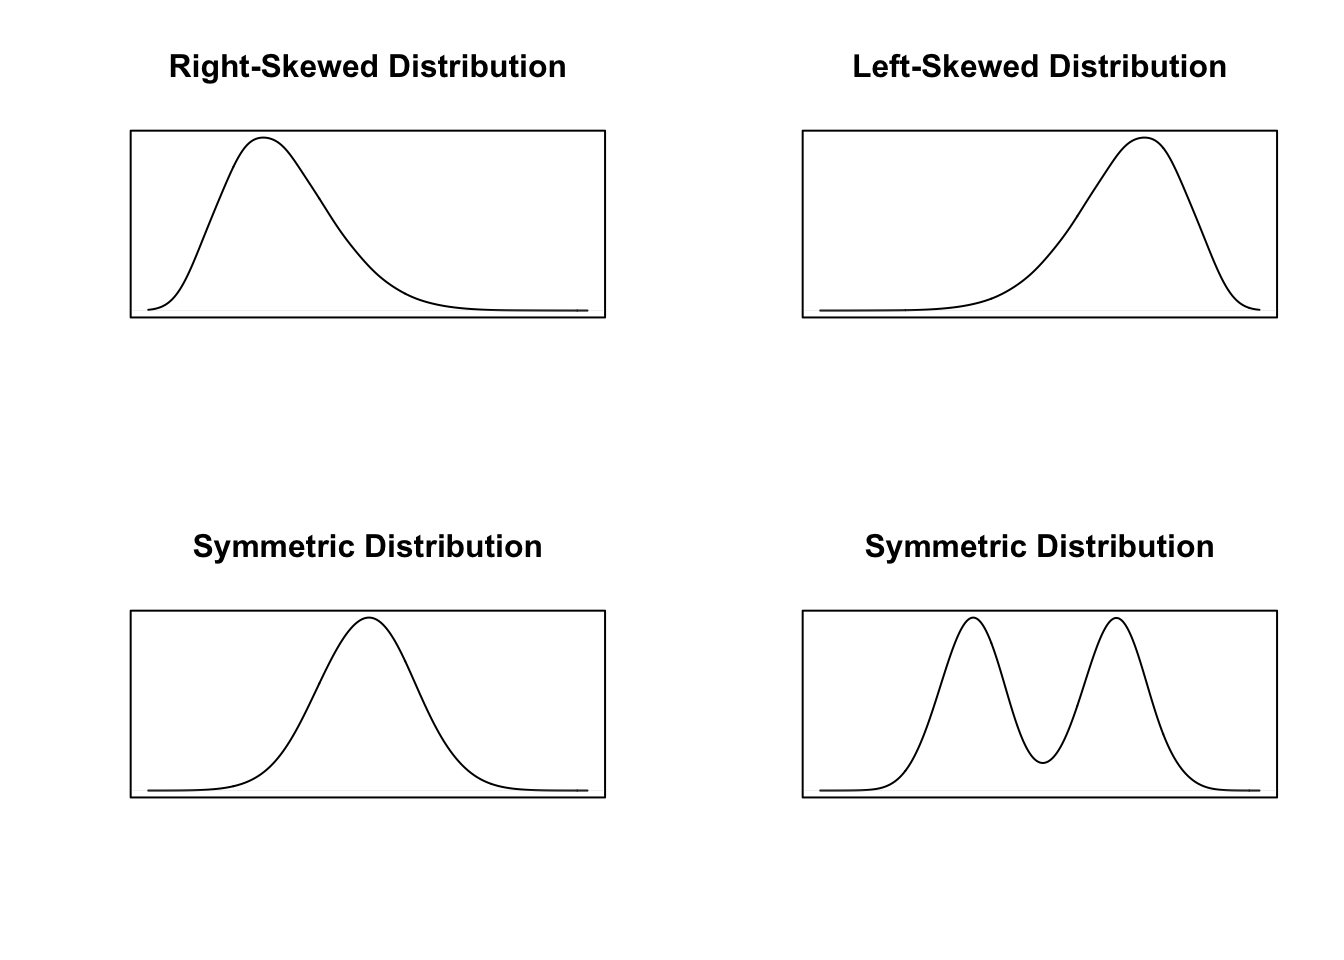
\includegraphics{IntroStats_files/figure-latex/unnamed-chunk-12-1.pdf}

\begin{quote}
Clearly, the relationship isn't perfectly linear, but there does appear to be some kind of linear relationship (as body length increases, head length also increases). We want to try to use body length (\(x\)) to predict head length (\(y\)).

The regression model for these data is \[\hat{y}=42.7 + 0.57x\]
\end{quote}

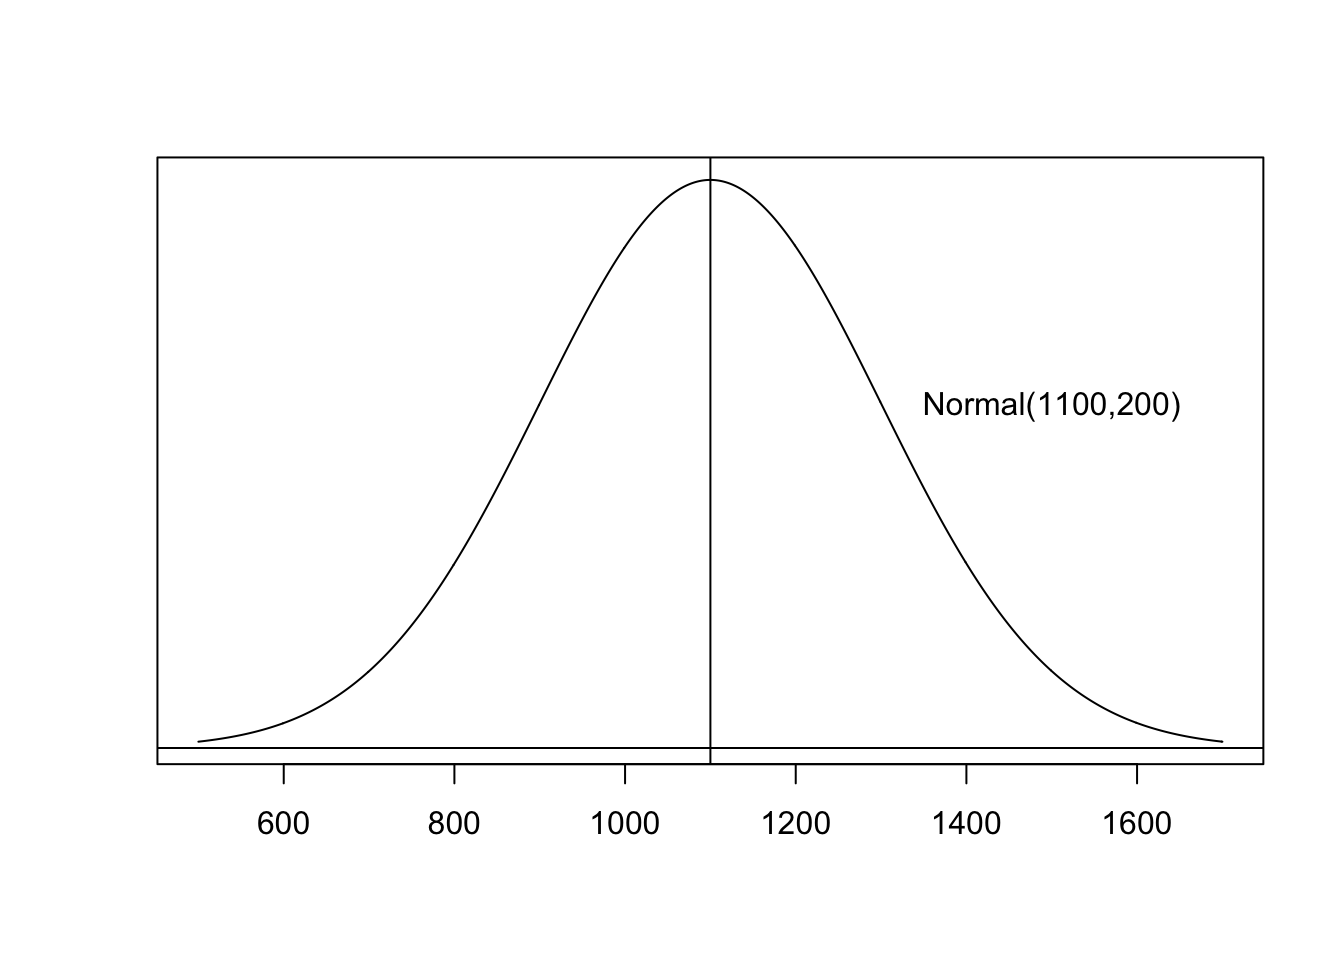
\includegraphics{IntroStats_files/figure-latex/unnamed-chunk-13-1.pdf}

\begin{quote}
To predict the head length for a possum with a body length of 80cm, we just need to plug in 80 for body length (\(x\)): \[\hat{y}=42.7 + 0.57(80) = 88.3\text{mm}.\] Note: because the regression line is built using the data's original units (cm for body length, mm for head length), the regression line will preserve those units. That means that when we plugged in a value in cm, the equation spit out a predicted value in mm.
\end{quote}

\hypertarget{correlation}{%
\subsection{Correlation}\label{correlation}}

We've talked about the strength of linear relationships, but it would be nice to formalize this concept. The \textbf{correlation} between two variables describes the strength of their linear relationship. It always takes values between -1 and 1. We denote the correlation (or correlation coefficient) by \(R\): \[R = \frac{1}{n-1}\sum_{i=1}^n\left(\frac{x_i - \bar{x}}{s_x}\times\frac{y_i - \bar{y}}{s_y}\right)\] where \(s_x\) and \(s_y\) are the respective standard deviations for \(x\) and \(y\). The sample size \(n\) is the total number of \((x,y)\) pairs.

\begin{quote}
\emph{Example}: Consider

\begin{longtable}[]{@{}cc@{}}
\toprule
\(x\) & \(y\) \\
\midrule
\endhead
1 & 3 \\
2 & 3 \\
3 & 4 \\
\(\bar{x} = 2\) & \(\bar{y} = 3.333\) \\
\(s_x = 1\) & \(s_y = 0.577\) \\
\bottomrule
\end{longtable}

Like we did with variance/standard deviation, I recommend using a table to calculate the correlation between \(x\) and \(y\):

\begin{longtable}[]{@{}
  >{\centering\arraybackslash}p{(\columnwidth - 8\tabcolsep) * \real{0.20}}
  >{\centering\arraybackslash}p{(\columnwidth - 8\tabcolsep) * \real{0.20}}
  >{\centering\arraybackslash}p{(\columnwidth - 8\tabcolsep) * \real{0.20}}
  >{\centering\arraybackslash}p{(\columnwidth - 8\tabcolsep) * \real{0.20}}
  >{\centering\arraybackslash}p{(\columnwidth - 8\tabcolsep) * \real{0.20}}@{}}
\toprule
\(x - \bar{x}\) & \(\frac{x - \bar{x}}{s_x}\) & \(y - \bar{y}\) & \(\frac{y - \bar{y}}{s_y}\) & \(\frac{x - \bar{x}}{s_x}\times\frac{y - \bar{y}}{s_y}\) \\
\midrule
\endhead
-1 & -1 & -0.333 & -0.577 & 0.577 \\
0 & 0 & -0.333 & -0.577 & 0.000 \\
1 & 1 & 0.667 & 1.155 & 1.155 \\
& & & & sum = 1.732 \\
\bottomrule
\end{longtable}

So \(R = \frac{1}{3-1}(1.732) = 0.866\)
\end{quote}

Correlations

\begin{itemize}
\tightlist
\item
  close to -1 suggest strong, negative linear relationships.
\item
  close to +1 suggest strong, positive linear relationships.
\item
  close to 0 have little-to-no linear relationship.
\end{itemize}

Note: the sign of the correlation will match the sign of the slope!

\begin{itemize}
\tightlist
\item
  If \(R < 0\), there is a downward trend and \(b_1 < 0\).
\item
  If \(R > 0\), there is an upward trend and \(b_1 > 0\).
\item
  If \(R \approx 0\), there is no relationship and \(b_1 \approx 0\).
\end{itemize}

A final note: correlations only represent \emph{linear} trends. Consider the following scatterplot:

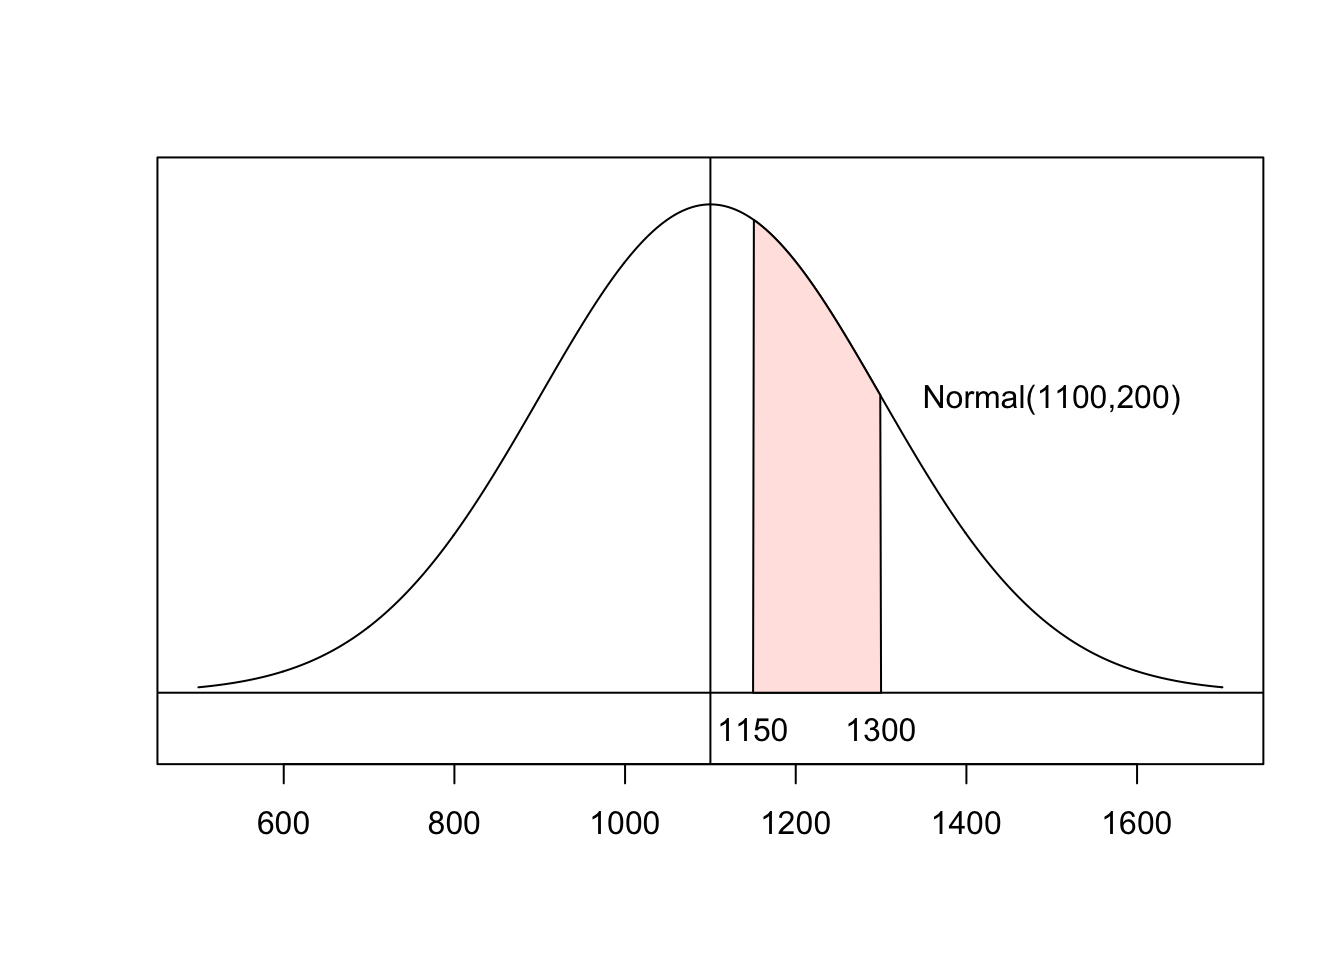
\includegraphics{IntroStats_files/figure-latex/unnamed-chunk-14-1.pdf}

Obviously there's a strong relationship between \(x\) and \(y\). In fact, there's a perfect relationship here: \(y = x^2\). But the \emph{correlation} between \(x\) and \(y\) is 0! This is one reason why it's important to examine the data both through visual and numeric measures.

\hypertarget{finding-a-regression-line}{%
\subsection{Finding a Regression Line}\label{finding-a-regression-line}}

\textbf{Residuals} are the leftover \emph{stuff} (variation) in the data after accounting for model fit: \[\text{data} = \text{prediction} + \text{residual}\] Each observation has its own residual. The residual for an observation \((x,y)\) is the difference between observed (\(y\)) and predicted (\(\hat{y}\)): \[e = y - \hat{y}\] We denote the residuals by \(e\) and find \(\hat{y}\) by plugging \(x\) into the regression equation. If an observation lands above the regression line, \(e > 0\). If below, \(e < 0\).

When we estimate the parameters for the regression, our goal is to get each residual as close to 0 as possible. We might think to try minimizing \[\sum_{i=1}^n e_i = \sum_{i=1}^n (y_i - \hat{y}_i)\] but that would just give us very large negative residuals. As with the variance, we will use squares to shift the focus to magnitude:
\begin{align}
\sum_{i=1}^n e_i^2 &= \sum_{i=1}^n (y_i - \hat{y}_i)^2 \\
& = \sum_{i=1}^n [y_i - (b_0 + b_1 x_i)]^2
\end{align}
This will allow us to shrink the residuals toward 0: the values \(b_0\) and \(b_1\) that minimize this will make up our regression line.

This is a calculus-free course, so we'll skip the proof of the minimization part. The slope can be estimated as \[b_1 = \frac{s_y}{s_x}\times R\] and the intercept as \[b_0 = \bar{y} - b_1 \bar{x}\]

\begin{quote}
\emph{Example}: Consider two measurements taken on the Old Faithful Geyser in Yellowstone National Park: \texttt{eruptions}, the length of each eruption and \texttt{waiting}, the time between eruptions. Each is measured in minutes.
\end{quote}

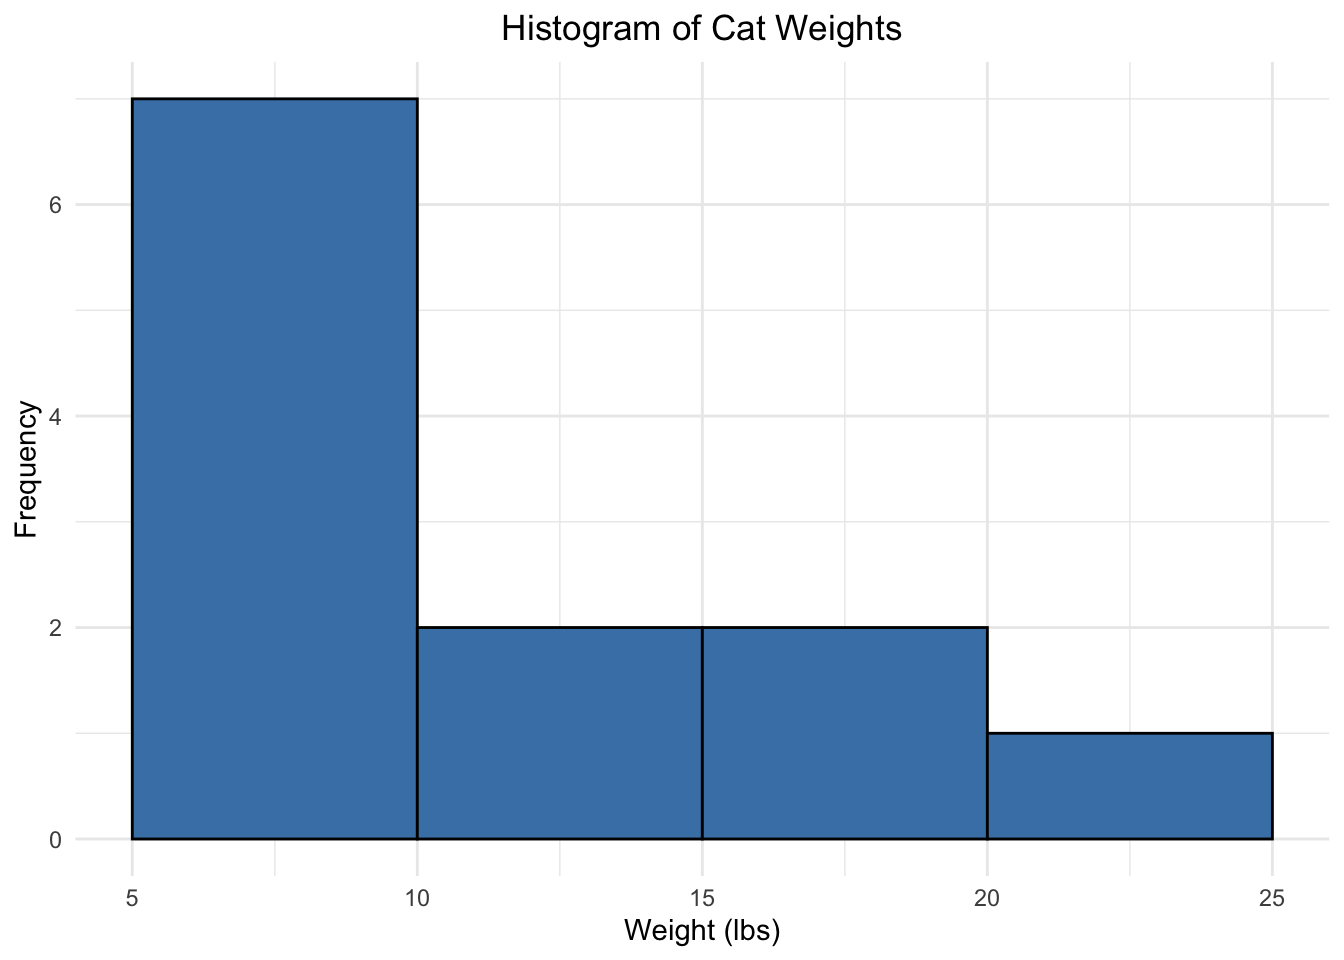
\includegraphics{IntroStats_files/figure-latex/unnamed-chunk-15-1.pdf}

\begin{quote}
There does appear to be some kind of linear relationship here, so we will see if we can use the wait time to predict the eruption duration. The sample statistics for these data are

\begin{longtable}[]{@{}ccc@{}}
\toprule
& \texttt{waiting} & \texttt{eruptions} \\
\midrule
\endhead
mean & \(\bar{x}=70.90\) & \(\bar{y}=3.49\) \\
sd & \(s_x=13.60\) & \(s_y=1.14\) \\
& & \(R = 0.90\) \\
\bottomrule
\end{longtable}

Since we want to use wait time to predict eruption duration, wait time is \(x\) and eruption duration is \(y.\) Then \[b_1 = \frac{1.14}{13.60}\times 0.90 \approx 0.076 \] and \[b_0 = 3.49 - 0.076\times 70.90 \approx -1.87\] so the estimated regression line is \[\hat{y} = -1.87 + 0.076x\]

To interpret \(b_1\), the slope, we would say that for a one-minute increase in waiting time, we would predict a 0.076 minute increase in eruption duration. The intercept is a little bit trickier. Plugging in 0 for \(x\), we get a predicted eruption duration of \(-1.87\) minutes. There are two issues with this. First, a negative eruption duration doesn't make sense\ldots{} but it also doesn't make sense to have a waiting time of 0 minutes.
\end{quote}

It's important to stop and think about our predictions. Sometimes, the numbers don't make sense and it's easy to see that there's something wrong with the prediction. Other times, these issues are more insidious. Usually, all of these issues result from what we call \emph{extrapolation}, applying a model estimate for values outside of the data's range for \(x\). Our linear model is only an approximation, and we don't know anything about how the relationship outside of the scope of our data!

Consider the following data with the best fit line drawn on the scatterplot.

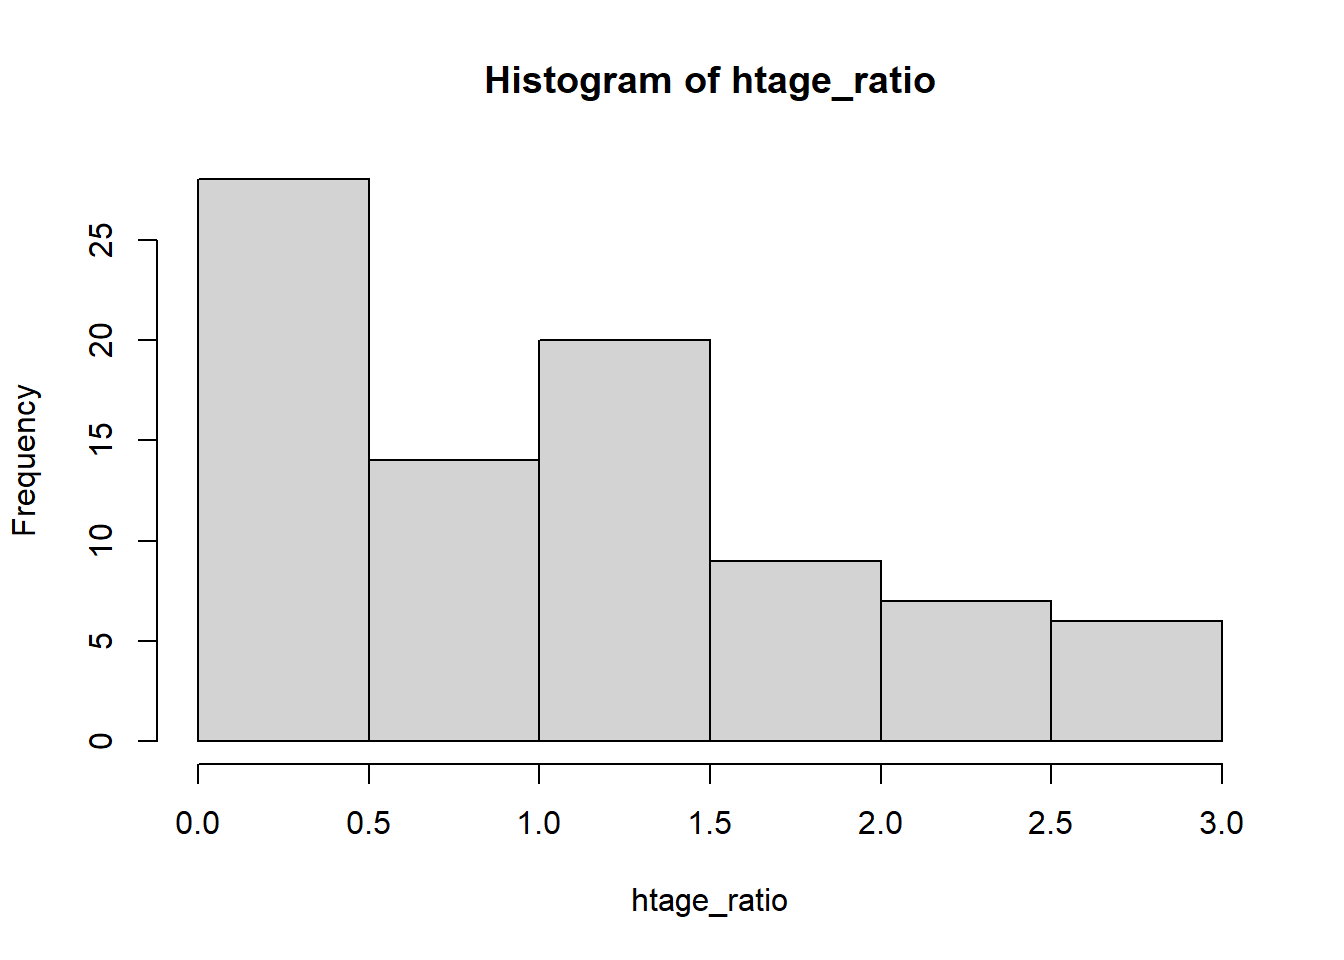
\includegraphics{IntroStats_files/figure-latex/unnamed-chunk-16-1.pdf}

The best fit line is \[\hat{y} = 2.66 + 0.181x\] and the correlation is \(R=0.832\), which is a reasonably strong positive linear correlation. Now suppose we wanted to predict the value of \(y\) when \(x=0.1\): \[\hat{y} = 2.66 + 0.181\times0.1 = 2.67\] This seems like a perfectly reasonable number\ldots{} But what if I told you that I generated the data using the model \(y = 2\ln(x) + \text{random error}\)? (If you're not familiar with the natural log, \(\ln\), don't worry about it! You won't need to use it.) The true (population) best-fit model would look like this:

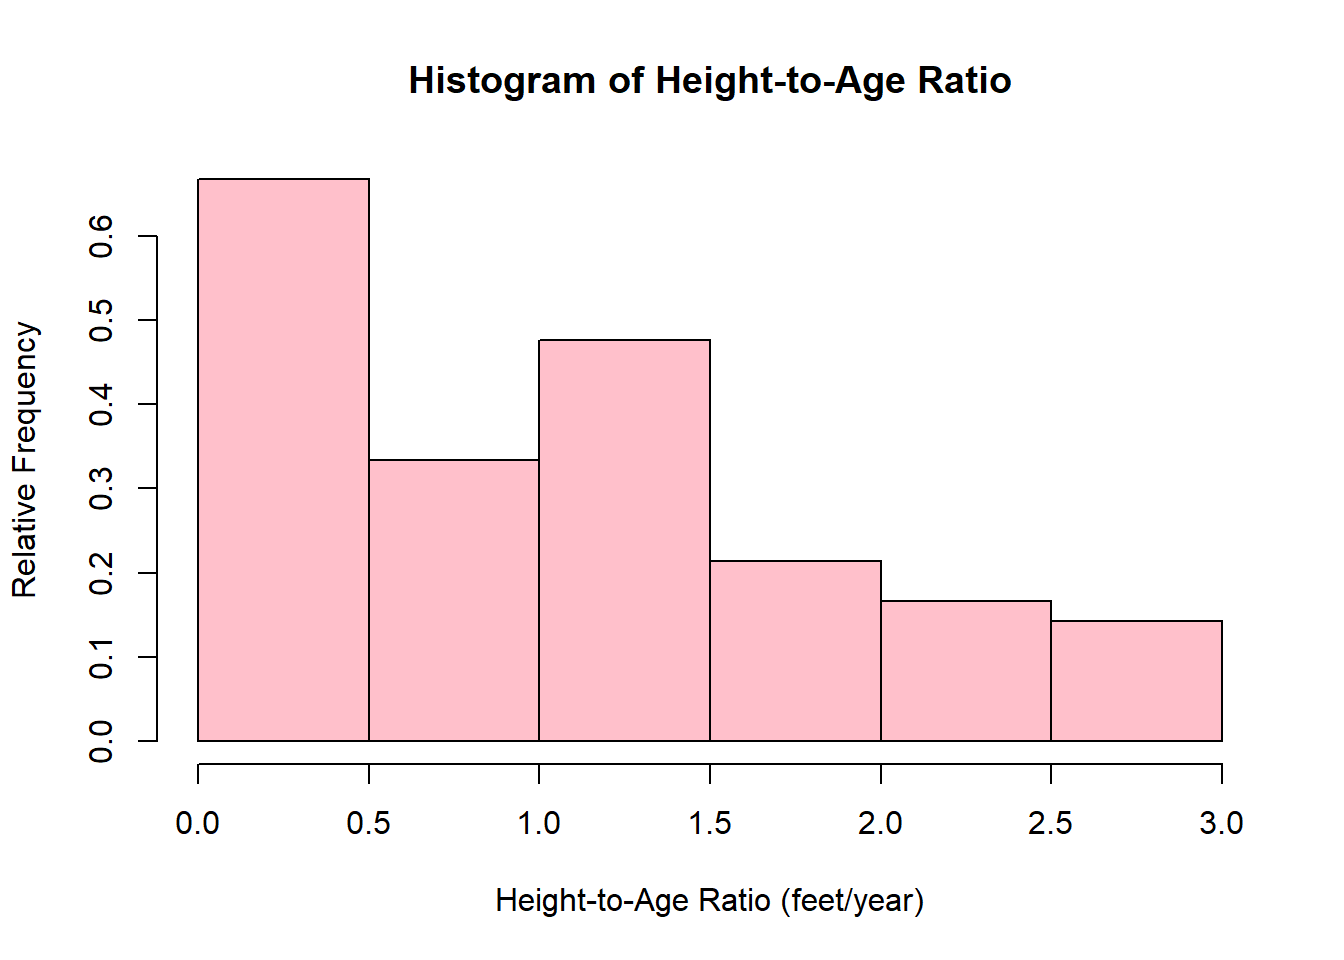
\includegraphics{IntroStats_files/figure-latex/unnamed-chunk-17-1.pdf}

The vertical lines at \(x=5\) and \(x=20\) show the bounds of our data. The blue dot at \(x=0.1\) is the predicted value \(\hat{y}\) based on the linear model. The dashed horizontal line helps demonstrate just how far this estimate is from the true population value! This does \emph{not} mean there's anything inherently wrong with our model. If it works well from \(x=5\) to \(x=20\), great, it's doing its job!

\hypertarget{probability-concepts}{%
\chapter{Probability Concepts}\label{probability-concepts}}

\hypertarget{module-overview-2}{%
\section{Module Overview}\label{module-overview-2}}

In previous modules, we discussed ways to describe variables and the relationships between them. From here, we want to start asking inferential statistics questions like ``If my sample mean is 10, how likely is it that the population mean is actually 11?''. Probability is going to start us on this path.

Probability theory is the science of uncertainty and it is really interesting! But it can also be quite challenging. I try to frame probability around things most of us can do at home: flipping a coin, rolling a die, drawing from a deck of cards. You certainly don't need any of these things to get through this module, but you may find it helpful to have a coin/die/deck of cards on hand as you read through the examples.

Take your time running practice problems (the solutions to odd-numbered problems are in the back of your textbook - these make great practice problems!).

\textbf{Module Learning Objectives/Outcomes}

\begin{enumerate}
\def\labelenumi{\arabic{enumi}.}
\tightlist
\item
  Find and interpret probabilities for equally likely events.
\item
  Find and interpret probabilities for events that are not equally likely.
\item
  Find and interpret joint and marginal probabilities.
\item
  Find and interpret conditional probabilities.
\item
  Use the multiplication rule and independence to calculate probabilities.
\end{enumerate}

This module's outcomes correspond to course outcome (3) understand the basic rules of probability.

\hypertarget{experiments-sample-spaces-and-events}{%
\section{Experiments, Sample Spaces, and Events}\label{experiments-sample-spaces-and-events}}

\textbf{Probability} is the science of uncertainty. When we run an experiment, we are unsure of what the outcome will be. Because of this uncertainty, we say an experiment is a \textbf{random process}.

The probability of an event is the proportion of times is would occur if the experiment were run infinitely many times:
\[
  \text{probability of event} = \frac{\text{number of ways event can occur}}{\text{number of possible (unique) outcomes}}
\]

An \textbf{event} is some specified possible outcome (or collection of outcomes) we are interested in observing.

\begin{quote}
\emph{Example}: If you want to roll a 6 on a six-sided die, there are six possible outcomes \(\{1,2,3,4,5,6\}\). So the probability of rolling a 6 is
\[
\frac{\text{number of ways to roll a 6}}{\text{number of possible rolls}} = \frac{1}{6}
\]
\end{quote}

\begin{quote}
\emph{Example}: We can extend this to a collection of events, say the probability of rolling a 5 or a 6:
\[
\frac{\text{number of ways to roll a 5 or 6}}{\text{number of possible rolls}} = \frac{2}{6}
\]
\end{quote}

The collection of all possible outcomes is called a \textbf{sample space}, denoted \(S\). For the six-sided die, \(S=\{1,2,3,4,5,6\}\).

To simplify our writing, we use \textbf{probability notation}:

\begin{itemize}
\tightlist
\item
  Events are assigned capital letters.
\item
  \(P(A)\) denotes the probability of event \(A\).
\end{itemize}

\hypertarget{probability-distributions}{%
\section{Probability Distributions}\label{probability-distributions}}

Two outcomes are \textbf{disjoint} or \textbf{mutually exclusive} if they cannot both happen (at the same time). Think back to how we developed bins for histograms - the bins need to be nonoverlapping - this is the same idea!

\begin{quote}
\emph{Example}: If I roll a six-sided die one time, rolling a 5 and rolling a 6 are disjoint. I can get a 5 \emph{or} a 6, but not both on the same roll.
\end{quote}

\hypertarget{venn-diagrams}{%
\subsection{Venn Diagrams}\label{venn-diagrams}}

\textbf{Venn Diagrams} show events as circles. The circles overlap where events share common outcomes.

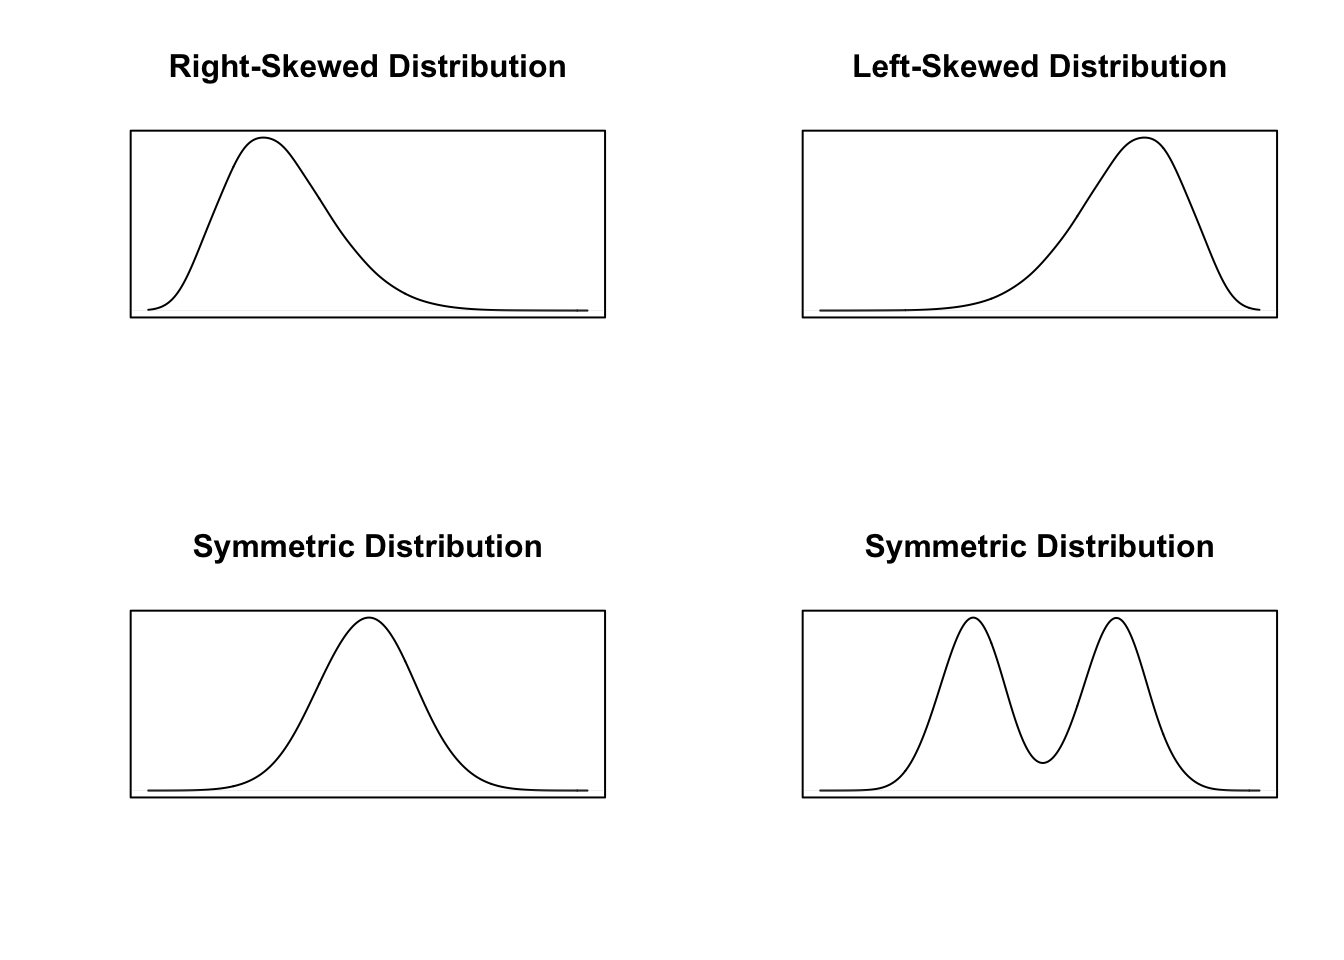
\includegraphics{IntroStats_files/figure-latex/unnamed-chunk-19-1.pdf}

When a Venn Diagram has \emph{no overlap} the events are mutually exclusive. This Venn Diagram shows the event ``Draw a Diamond'' and the event ``Draw a Face Card''. There are 13 diamonds and 12 face cards in a deck. In this case, the events are \emph{not} mutually exclusive: it's possible to draw both a diamond and a face card at the same time: the Jack of Diamonds, Queen of Diamonds, and Kind of Diamonds.

For quick reference, a full 52-card deck is shown below. The ``face cards'' are the J, Q, and K. Each row represents a ``suit''. From top to bottom, the suits are clubs, spades, hearts, and diamonds. Cards can be either red (hearts and diamonds) or black (spades and clubs).

\href{https://www.cis.upenn.edu/~cis110/17fa/hw/hw08/standard52.jpg}{Click here for a graphic of a standard 52 card deck.}

\emph{On your own}: Consider events

\begin{itemize}
\tightlist
\item
  \(A\): ``Draw a spade''
\item
  \(B\): ``Draw a queen''
\item
  \(C\): ``Draw a red''
\end{itemize}

Which of these events are mutually exclusive?

A \textbf{probability distribution} lists all possible disjoint outcomes (think: all possible values of a variable) and their associated probabilities. This can be in the form of a table

\begin{longtable}[]{@{}ccccccc@{}}
\toprule
Roll of a six-sided die & 1 & 2 & 3 & 4 & 5 & 6 \\
\midrule
\endhead
Probability & 1/6 & 1/6 & 1/6 & 1/6 & 1/6 & 1/6 \\
\bottomrule
\end{longtable}

(note that we could visualize this with a bar plot!) or an equation, which we will discuss in a later module.

\hypertarget{probability-axioms}{%
\subsection{Probability Axioms}\label{probability-axioms}}

\begin{enumerate}
\def\labelenumi{\arabic{enumi}.}
\tightlist
\item
  All listed outcomes must be disjoint.
\item
  Each probability must be between 0 and 1.
\item
  The probabilities must sum to 1.
\end{enumerate}

These are the requirements for a valid probability distribution. Note that \#2 is true for ALL probabilities. If you ever calculate a probability and get a negative number or a number greater than 1, you know something went wrong!

\begin{quote}
\emph{Example}: Use the probability axioms to check whether the following tables are probability distributions.

\begin{longtable}[]{@{}cccc@{}}
\toprule
X & \{1 or 2\} & \{3 or 4\} & \{5 or 6\} \\
\midrule
\endhead
P(X) & 1/3 & 1/3 & 1/3 \\
\bottomrule
\end{longtable}

Each axiom is satisfied, so this is a valid probability distribution.

\begin{longtable}[]{@{}ccccc@{}}
\toprule
Y & \{1 or 2\} & \{2 or 3\} & \{3 or 4\} & \{5 or 6\} \\
\midrule
\endhead
P(Y) & 1/3 & 1/3 & 1/3 & -1/3 \\
\bottomrule
\end{longtable}

In this case, the outcomes are not disjoint and one of the probabilities is negative, so this is \emph{not} a valid probability distribution.
\end{quote}

\hypertarget{rules-of-probability}{%
\section{Rules of Probability}\label{rules-of-probability}}

Consider a six-sided die. \[P(\text{roll a 1 or 2}) = \frac{\text{2 ways}}{\text{6 outcomes}} = \frac{1}{3}.\] Notice that we get the same result by taking \[P(\text{roll a 1})+P(\text{roll a 2}) = \frac{1}{6}+\frac{1}{6} = \frac{1}{3}.\] It turns out this is widely applicable!

\hypertarget{addition-rules}{%
\subsection{Addition Rules}\label{addition-rules}}

\textbf{Addition Rule for Disjoint Outcomes}

If \(A_1\) and \(A_2\) are disjoint outcomes, then the probability that one of them occurs is \[P(A_1 \text{ or } A_2) = P(A_1)+P(A_2).\] This can also be extended to more than two disjoint outcomes: \[P(A_1 \text{ or } A_2 \text{ or } \dots \text{ or } A_k) = P(A_1)+P(A_2)+\dots + P(A_k)\] for \(k\) disjoint outcomes.

Now consider a deck of cards. Let \(A\) be the event that a card drawn is a diamond and let \(B\) be the event it is a face card. (Check back to 3.2 for the Venn Diagram of these events - they are \emph{not} disjoint!).

Here \(P(A)=\frac{13}{52}\) and \(P(B)=\frac{12}{52}\). If we add these, we \emph{double count} the Jack of Diamonds, Queen of Diamonds, and King of Diamonds. So we need to account for that: \(\frac{13}{52}+\frac{12}{52}-\frac{3}{52}\).

\textbf{General Addition Rule}

For any two events \(A\) and \(B\), the probability that \emph{at least} one will occur is \[P(A \text{ or } B) = P(A)+P(B)-P(A \text{ and }B).\]

Notice that when we say ``or'', we include the situations where A is true, B is true, and the situation where are both A and B are true. This is an \emph{inclusive or}. Basically, if I said ``Do you like cats or dogs?'' and you said ``Yes.'' because you like cats \emph{and} dogs, that would be a perfectly valid response. I recommend using the inclusive or with your friends any time you want to get out of making a decision.

\hypertarget{complements}{%
\subsection{Complements}\label{complements}}

The \textbf{complement} of an event is all of the outcomes in the sample space that are \emph{not} in the event.

\begin{quote}
\emph{Example}: For a single roll of a six-sided die, the sample space is all possible rolls: 1, 2, 3, 4, 5, or 6. If the event \(A\) is rolling a 1 or a 2, then the complement of this event, denoted \(A^c\), is rolling a 3, 4, 5, or 6. We could also write this in probability notation: \(S = \{1, 2, 3, 4, 5, 6\}\) and if \(A=\{1,2\}\), then \(A^c=\{3, 4, 5, 6\}\).
\end{quote}

\textbf{Property}: \[P(A \text{ or } A^c)=1\] Using the addition rule, \[P(A \text{ or } A^c) = P(A)+P(A^c) = 1.\] (Make sure you can convince yourself that \(A\) and \(A^c\) are \emph{always} disjoint.) This is especially useful written as \[P(A) = 1-P(A^c).\]

\begin{quote}
\emph{Example}: Consider rolling 2 six-sided dice and taking their sum. The event of interest is a sum less than 12. Find

\begin{enumerate}
\def\labelenumi{\arabic{enumi}.}
\tightlist
\item
  \(A^c\)
\item
  \(P(A^c)\)
\item
  \(P(A)\)
\end{enumerate}

If \(A =\) (sum less than 12), then \(A^c =\) (sum greater than or equal to 12). Take a moment to notice that there is only one way to get a sum greater than or equal to 12: rolling two 6s. The chart below shows the rolls of Die 1 as columns and the rolls for Die 2 as rows. The numbers in the middle are the sums. Notice that there are 36 possible ways to roll 2 dice.

\begin{longtable}[]{@{}lcccccc@{}}
\toprule
& 1 & 2 & 3 & 4 & 5 & 6 \\
\midrule
\endhead
1 & 2 & 3 & 4 & 5 & 6 & 7 \\
2 & 3 & 4 & 5 & 6 & 7 & 8 \\
3 & 4 & 5 & 6 & 7 & 8 & 9 \\
4 & 5 & 6 & 7 & 8 & 9 & 10 \\
5 & 6 & 7 & 8 & 9 & 10 & 11 \\
6 & 7 & 8 & 9 & 10 & 11 & 12 \\
\bottomrule
\end{longtable}

\[ P(A^c) = \frac{1}{36}\]
Then \[P(A) = 1 - P(A^c) = 1-\frac{1}{36} = \frac{35}{36}\] which is a much faster way to calculate this than to count up all the times the sum is less than 12!
\end{quote}

\hypertarget{conditional-probability}{%
\section{Conditional Probability}\label{conditional-probability}}

A \textbf{contingency table} is a way to summarize \textbf{bivariate data}, or data from two variables.

\emph{Smallpox in Boston (1726)}

~

Inoculated

~

yes

no

total

Result

lived

238

{5136}

{5374}

died

6

855

850

total

{244}

5980

{6224}

{5136} is the count of people who lived AND were not inoculated.~

{6224} is the total number of observations.

{244} is the total number of people who were inoculated.

{5374} is the total number of people who lived.

This is like a two-way frequency distribution. Like a frequency distribution, we can convert to proportions by dividing each count by the total number of observations:

~

Inoculated

~

yes

no

total

Result

lived

0.0382

{0.8252}

{0.8634}

died

0.0010

0.1356

0.1366

total

{0.0392}

0.9608

{1.0000}

{0.8252} is the proportion of people who lived AND were not inoculated.~

{1.000} is the proportion of total number of observations. Think of this as 100\% of the observations.

{0.0392} is the proportion of people who were inoculated.

{0.8634} is the proportion of people who lived.

The row and column totals are \textbf{marginal probabilities}. The probability of two events together (\(A\) and \(B\)) is a \textbf{joint probability}.

What can we learn about the result of smallpox if we already know something about inoculation status? For example, given that a person is inoculated, what is the probability of death? To figure this out, we restrict our attention to the 244 inoculated cases. Of these, 6 died. So the probability is 6/244.

This is called \textbf{conditional probability}, the probability of some event \(A\) given that event \(B\) occurs: \[P(A|B) = \frac{P(A\text{ and }B)}{P(B)}\] where the symbol \textbar{} is read as ``given''.

\begin{quote}
For death given inoculation, \[P(\text{death}|\text{inoculation}) = \frac{P(\text{death and inoculation})}{P(\text{death})} = \frac{0.0010}{0.0392} = 0.0255.\]
Notie that we could also write this as \[P(\text{death}|\text{inoculation}) = \frac{P(\text{death and inoculation})}{P(\text{death})} = \frac{6/6224}{244/6224} = \frac{6}{244},\] which is what we found when using the table to restrict our attention to only the inoculated cases.
\end{quote}

If knowing whether event \(B\) occurs tells us nothing about event \(A\), the events are \textbf{independent}. For example, if we know that the first flip of a (fair) coin came up heads, that doesn't tell us anything about what will happen next time we flip that coin.

We can test for independence by checking if \(P(A|B)=P(A)\).

\hypertarget{multiplication-rules}{%
\subsection{Multiplication Rules}\label{multiplication-rules}}

\textbf{Multiplication Rule for Independent Processes}

If \(A\) and \(B\) are independent events, then \[P(A \text{ and }B) = P(A)P(B).\]

We can extend this to more than two events: \[P(A \text{ and }B \text{ and } C \text{ and } \dots) = P(A)P(B)P(C)\dots.\]

Note that if \(P(A \text{ and }B) \ne P(A)P(B)\), then \(A\) and \(B\) are \emph{not} independent.

\textbf{General Multiplication Rule}

If \(A\) and \(B\) are any two events, then \[P(A \text{ and }B) = P(A|B)P(B).\]

Notice that this is just the conditional probability formula, rewritten in terms of \(P(A \text{ and }B)\)!

\hypertarget{random-variables}{%
\chapter{Random Variables}\label{random-variables}}

\hypertarget{module-overview-3}{%
\section{Module Overview}\label{module-overview-3}}

In previous modules, we introduced the idea of variables and examined their distributions. We also began our discussion on probability theory. Now, we extend these concepts into what are called random variables. We will introduce the concept of random variables in general and will discuss a specific type of distribution - the binomial distribution. Then we will discuss a continuous probability distribution, the normal distribution. The normal distribution will provide a foundation for much of the inference we will complete throughout the rest of this course.

\textbf{Module Learning Objectives/Outcomes}

\begin{enumerate}
\def\labelenumi{\arabic{enumi}.}
\tightlist
\item
  Discuss discrete random variables using key terminology.
\item
  Express cumulative probabilities using probability notation.
\item
  Calculate the expected value and standard deviation of a discrete random variable.
\item
  Calculate binomial probabilities.
\item
  Convert normal distributions to standard normal distributions.
\item
  Calculate probabilities for a normal distribution using area under the curve.
\item
  Approximate binomial probabilities using the normal curve.
\end{enumerate}

This module's outcomes correspond to course outcomes (4) use the binomial distribution as a model for discrete variables and (5) use the normal distribution as a model for continuous variables.

\hypertarget{discrete-random-variables}{%
\section{Discrete Random Variables}\label{discrete-random-variables}}

A \textbf{random variable} is a quantitative variable whose values are based on chance. By ``chance'', we mean that you can't \emph{know} the outcome before it occurs.

A \textbf{discrete random variable} is a random variable whose possible values can be listed.

Notation:

\begin{itemize}
\tightlist
\item
  \(x\),\(y\),\(z\) (lower case letters) denote variables.
\item
  \(X\), \(Y\), \(Z\) (upper case letters) denote \emph{random} variables.
\end{itemize}

In contrast to events, where we usually used letters toward the start of the alphabet, (random) variables are typically denoted by letters from the end of the alphabet.

\begin{itemize}
\tightlist
\item
  \(\{X=x\}\) denotes the event that the random variable \(X\) equals \(x\).
\item
  \(P(X=x)\) denotes the probability that the random variable \(X\) equals \(x\).
\end{itemize}

Recall: a probability distribution is a list of all possible values and their corresponding probabilities. (See Section 3.3 for a refresher.) A \textbf{probability histogram} is a histogram where the heights of the bars correspond to the probability of each value. For discrete random variables, each ``bin'' is one of the listed values.

\begin{quote}
\emph{Example}:

\begin{longtable}[]{@{}lccccc@{}}
\toprule
Number of Siblings, \(x\) & 0 & 1 & 2 & 3 & 4 \\
\midrule
\endhead
\textbf{Probability}, \(P(X=x)\) & 0.200 & 0.425 & 0.275 & 0.075 & 0.025 \\
\bottomrule
\end{longtable}

(Assume for the sake of the example that no one has more than 4 siblings.)
\end{quote}

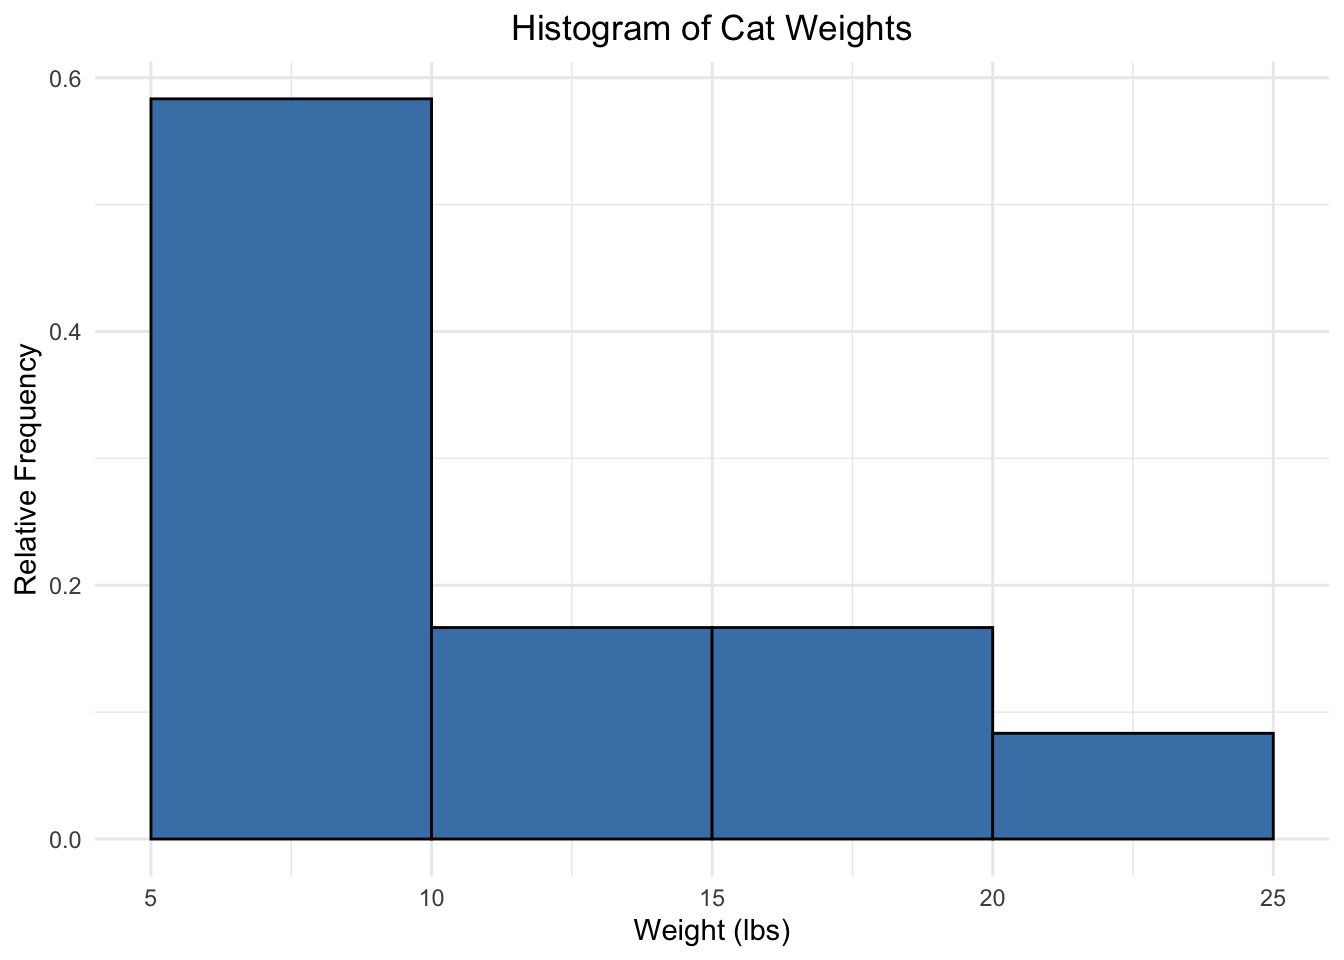
\includegraphics{IntroStats_files/figure-latex/unnamed-chunk-20-1.pdf}

Interpretation: in a large number of independent observations of a random variable \(X\), the proportion of times each possible value occurs will approximate the probability distribution of \(X\).

\hypertarget{the-mean-and-standard-deviation}{%
\subsection{The Mean and Standard Deviation}\label{the-mean-and-standard-deviation}}

\textbf{Mean of a Discrete Random Variable}

The mean of a discrete random variable \(X\) is denoted \(\mu_X\). If it's clear which random variable we're talking about, we can drop the subscript and write \(\mu\).
\[
  \mu_X = \Sigma xP(X=x)
\]
where \(\Sigma\) denotes ``the sum over all values of \(x\)'': \[\Sigma xP(X=x) = x_1P(X=x_1) + x_2P(X=x_2) + \dots + x_nP(X=x_n).\]

The mean of a random variable is also called the \textbf{expected value} or \textbf{expectation}. Recall that measures of center are meant to identify the most common or most likely, thus the value we can \emph{expect} to see (most often).

\begin{quote}
\emph{Example}: for the Siblings distribution, \[\mu = 0(0.200)+1(0.425)+2(0.275)+3(0.075)+4(0.025)=1.3\]
Make sure you understand how we used the formula for \(\mu\) and the probability distribution to come up with this number.
\end{quote}

Interpretation: in a large number of independent observations of a random variable \(X\), the mean of those observations will approximately equal \(\mu\).

The larger the number of observations, the closer their average tends to be to \(\mu\). This is known as the \textbf{law of large numbers}.

\begin{quote}
\emph{Example}: Suppose I took a random sample of 10 people and asked how many siblings they have. \[2,2,2,2,1,0,3,1,2,0\] In my random sample of 10, \(\bar{x}=2\), which is a reasonable estimate but not that close to the true mean \(\mu=1.3\).

\begin{itemize}
\tightlist
\item
  A random sample of 30 gave me a mean of \(\bar{x}=1.53\).
\item
  A random sample of 100 gave me a mean of \(\bar{x}=1.47\).
\item
  A random sample of 1000 gave me a mean of \(\bar{x}=1.307\).
\end{itemize}
\end{quote}

We use concepts related to the law of large numbers as a foundation for statistical inference, but note that - although very large samples are nice to have - it's not necessary to take enormous samples all the time. Often, we can come to interesting conclusions with fewer than 30 observations!

\textbf{Standard Deviation of a Discrete Random Variable}

The variance of a discrete random variable \(X\) is denoted \(\sigma_X^2\) (or \(\sigma^2\) if it's clear which variable we're talking about).
\[ \sigma_X^2 = \Sigma[(x-\mu_X)^2P(X=x)]\]
OR
\[ \sigma_X^2 = \Sigma[x^2P(X=x)]-\mu_X^2\]
These formulas are \emph{exactly} equivalent and you may use whichever you wish, but note that the second may be a little easier to work with.

As before, the standard deviation is the square root of the variance: \[\sigma = \sqrt{\sigma^2}\]

\begin{quote}
\emph{Example}: Calculate the standard deviation of the Siblings variable.

In general, a table is the best way to keep track of a variance calculation:

\begin{longtable}[]{@{}ccccc@{}}
\toprule
\(x\) & \(P(X=x)\) & \(xP(X=x)\) & \(x^2\) & \(x^2P(X=x)\) \\
\midrule
\endhead
0 & 0.200 & 0 & 0 & 0 \\
1 & 0.425 & 0.425 & 1 & 0.425 \\
2 & 0.275 & 0.550 & 4 & 1.100 \\
3 & 0.075 & 0.225 & 9 & 0.675 \\
4 & 0.025 & 0.100 & 16 & 0.400 \\
& & \(\mu\) = 1.3 & & Total = 2.6 \\
\bottomrule
\end{longtable}

Then the variance is \[\sigma^2 = 2.6 - 1.3^2 = 0.9\] and the standard deviation is \[\sigma = \sqrt{0.9} = 0.9539.\]
\end{quote}

\hypertarget{the-binomial-distribution}{%
\section{The Binomial Distribution}\label{the-binomial-distribution}}

Think back to replication in an experiment. Each replication is what we call a \textbf{trial}. We will consider a setting where each trial has two possible outcomes.

\begin{quote}
For example, suppose you want to know if a coin is fair (both sides equally likely). You might flip the coin 100 times (thus running 100 trials). Each trial is a flip of the coin with two possible outcomes: heads or tails.
\end{quote}

The product of the first \(k\) positive integers \((1, 2, 3, \dots)\) is called \textbf{k-factorial}, denoted \(k!\): \[k! = k \times (k-1) \times\dots\times 3 \times 2 \times 1\] We define \(0!=1\).

\begin{quote}
\emph{Example}: \(5! = 5 \times 4 \times 3 \times 2 \times 1 = 120\)
\end{quote}

If \(n\) is a positive integer \((1, 2, 3, \dots)\) and \(x\) is a nonnegative integer \((0, 1, 2, \dots)\) with \(x \le n\), the \textbf{binomial coefficient} is \[\binom{n}{x} = \frac{n!}{x!(n-x)!}\]

\begin{quote}
\emph{Example}: \[\binom{5}{2} = \frac{5!}{2!(5-2)!} = \frac{5 \times 4 \times 3 \times 2 \times 1}{(2 \times 1)(3 \times 2 \times 1)}\]
\end{quote}

Sometimes, we may want to simplify a binomial coefficient \emph{before} taking all of the factorials. Why? Well, \[20! = 2432902008176640000\] Most calculators will not print this number. Instead, you'll get an error or a rounded version printed using scientific notation. Neither will help you accurately calculate the binomial coefficient.

\begin{quote}
\emph{Example}: \[\binom{20}{17} = \frac{20\times 19\times 18\times 17\times 16\times \dots \times 3\times 2\times 1}{(17\times 16\times \dots \times 3\times 2\times 1)(3\times 2\times 1)}\] but notice that I can rewrite \(20!\) as \(20\times 19\times 18\times 17!\), so \[\binom{20}{17} = \frac{20\times 19\times 18\times 17!}{17!(3\times 2\times 1)} = \frac{20\times 19\times 18}{3\times 2\times 1} = \frac{6840}{6} = 1140\]
\end{quote}

\textbf{Bernoulli trials} are repeated trials of an experiment that satisfy
1. Each trial has two possible outcomes: success and failure.
2. Trials are independent.
3. The probability of success (the \textbf{success probability}) \(p\) remains the same from one trial to the next: \[P(X=\text{success})=p\]

The \textbf{binomial distribution} is the probability distribution for the number of successes in a sequence of Bernoulli trials.

Fact: in \(n\) Bernoulli trials, the number of outcomes that contain exactly \(x\) successes equals the binomial coefficient \(\binom{n}{x}\).

\textbf{Binomial Probability Formula}

Let \(x\) denote the total number of successes in \(n\) Bernoulli trials with success probability \(p\). The probability distribution of the random variable \(X\) is given by \[P(X=x) = \binom{n}{x}p^x(1-p)^{n-x} \quad\quad x = 0,1,2,\dots,n\] The random variable \(X\) is called a \textbf{binomial random variable} and is said to have the \textbf{binomial distribution}. Because \(n\) and \(p\) fully define this distribution, they are called the distribution's \textbf{parameters}.

To find a binomial probability formula:

Check assumptions.

Exactly \(n\) trials to be performed.

Two possible outcomes for each trial.

Trials are independent (each trial does not impact the result of the next)

Success probability \(p\) remains the same from trial to trial.

Identify a ``success''. Generally, this is whichever of the two possible outcomes we are most interested in.

Determine the success probability \(p\).

Determine \(n\), the number of trials.

Plug \(n\) and \(p\) into the binomial distribution formula.

We can also use the binomial probability formula to calculate probabilities like \(P(X\le x)\). Notice that we can rewrite this uisng concepts from the previous module \[P(X \le k) = P(X=k \text{ or } X=k-1 \text{ or } \dots  \text{ or } X=2 \text{ or } X=1  \text{ or } X=0)\] Since \(X\) is a discrete random variable, each possible value is \emph{disjoint}. We can use this! \[P(X \le k) = P(X=k) + P(X=k-1) + \dots + P(X=2) + P(X=1) + P(X=0)\]

\begin{quote}
\emph{Example}: \(P(X \le 3) = p(X=3)+P(X=2)+P(X=1)+P(X=0)\)
\end{quote}

We can also extend this concept to work with probabilities like \(P(a < X \le b)\).

\begin{quote}
\emph{Example}: \(P(2 < X \le 5)\)

First, notice that if \(2 < X \le 5\), then \(X\) can be 3, 4, or 5: \[P(2 < X \le 5) = P(X=3)+P(X=4)+P(X=5)\]
\end{quote}

\begin{quote}
Note: if going from \(2 < X \le 5\) to ``\(X\) can be 3, 4, or 5'' doesn't make sense to you, start by writing out the sample space. Suppose \(n=10\). Then the sample space for the binomial distribution is \[S = \{0, 1, 2, 3, 4, 5, 6, 7, 8, 9, 10\}\] Then I can check any number in this sample space by plugging it in for \(X\). So for 1, I can check \(2 < 1 \le 5\). Obviously this is not true, so we won't include 1. Checking the number 2, I get \(2 < 2 \le 5\). Since 2 \textless{} 2 is NOT true, we don't include 2. Etc.
\end{quote}

\hypertarget{mean-and-variance}{%
\subsection{Mean and Variance}\label{mean-and-variance}}

The shape of a binomial distribution is determined by the success probability:

\begin{itemize}
\tightlist
\item
  If \(p \approx 0.5\), the distribution is approximately symmetric.
\item
  If \(p < 0.5\), the distribution is right-skewed.
\item
  If \(p > 0.5\), the distribution is left-skewed.
\end{itemize}

The mean of a binomial distribution is \(\mu = np\). The variance is \(\sigma^2 = np(1-p)\).

\hypertarget{the-normal-distribution}{%
\section{The Normal Distribution}\label{the-normal-distribution}}

If we can represent a discrete variable with a probability histogram, what can we do with a continuous variable?

We represent the shape of a continuous variable using a \textbf{density curve}. This is like a histogram, but with a smooth curve:
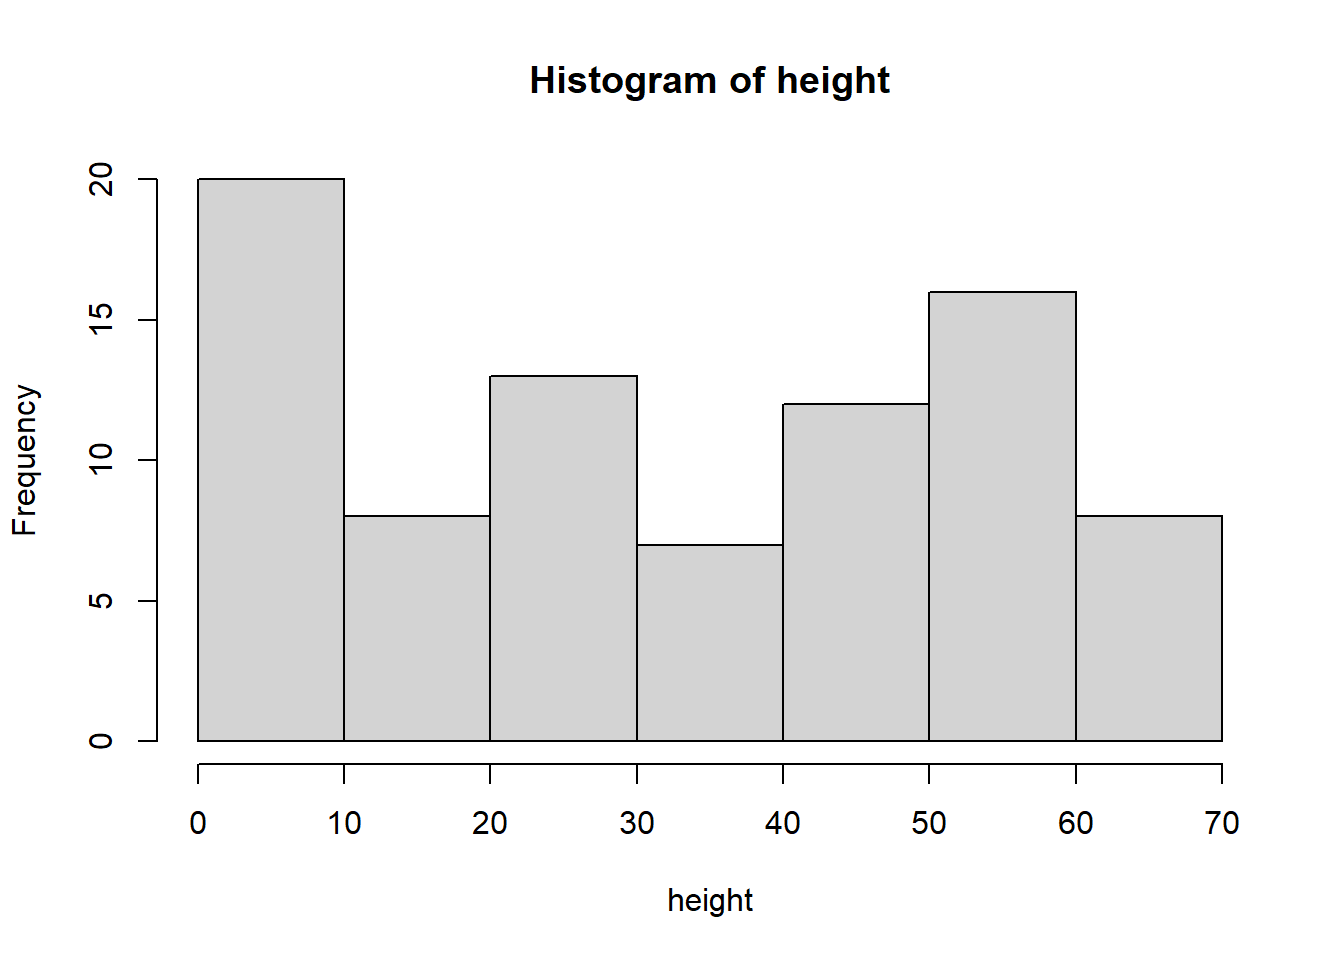
\includegraphics{IntroStats_files/figure-latex/unnamed-chunk-21-1.pdf}

Properties:

\begin{enumerate}
\def\labelenumi{\arabic{enumi}.}
\tightlist
\item
  The curve is always above the horizontal axis (because probabilities are always nonnegative).
\item
  The total area under the curve equals 1.
\end{enumerate}

For a variable with a density curve, the proportion of all possible observations that lie within a specified range equals the corresponding area under the density curve.

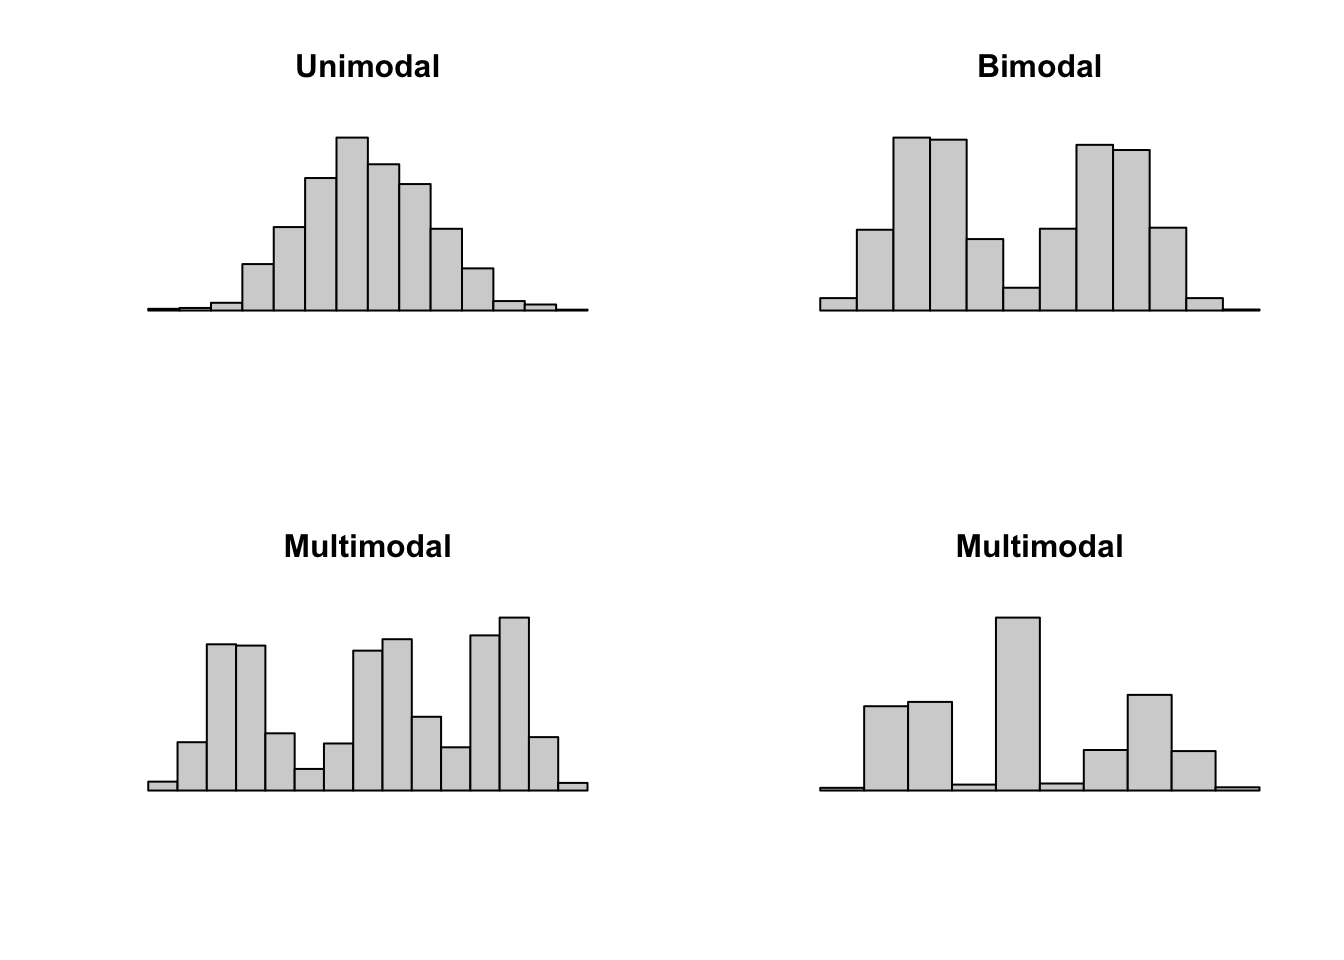
\includegraphics{IntroStats_files/figure-latex/unnamed-chunk-22-1.pdf}

A \textbf{normal curve} is a special type of density curve that has a ``bell-shaped'' distribution. In fact, all of the density curves I've shown so far have been normal curves! We say that a variable is \textbf{normally distributed} or has a \textbf{normal distribution} if its distribution has the shape of a normal curve.

Why ``normal''? Because it's very common! Lots of things are more common around the average and less common as you get farther from the average: height, amount of sleep people get each night, standardized test scores, etc. In practice, these things aren't \emph{exactly} normally distributed\ldots{} instead, they're \textbf{approximately normally distributed} (and that's ok).

Normal distributions\ldots{}

\begin{itemize}
\tightlist
\item
  are fully determined by parameters mean \(\mu\) and standard deviation \(\sigma\).
\item
  are symmetric and centered at \(\mu\).
\item
  have spreads that depend on \(\sigma\).
\end{itemize}

Pay close attention to the horizontal axis and how spread out the densities are in each of the following plots:

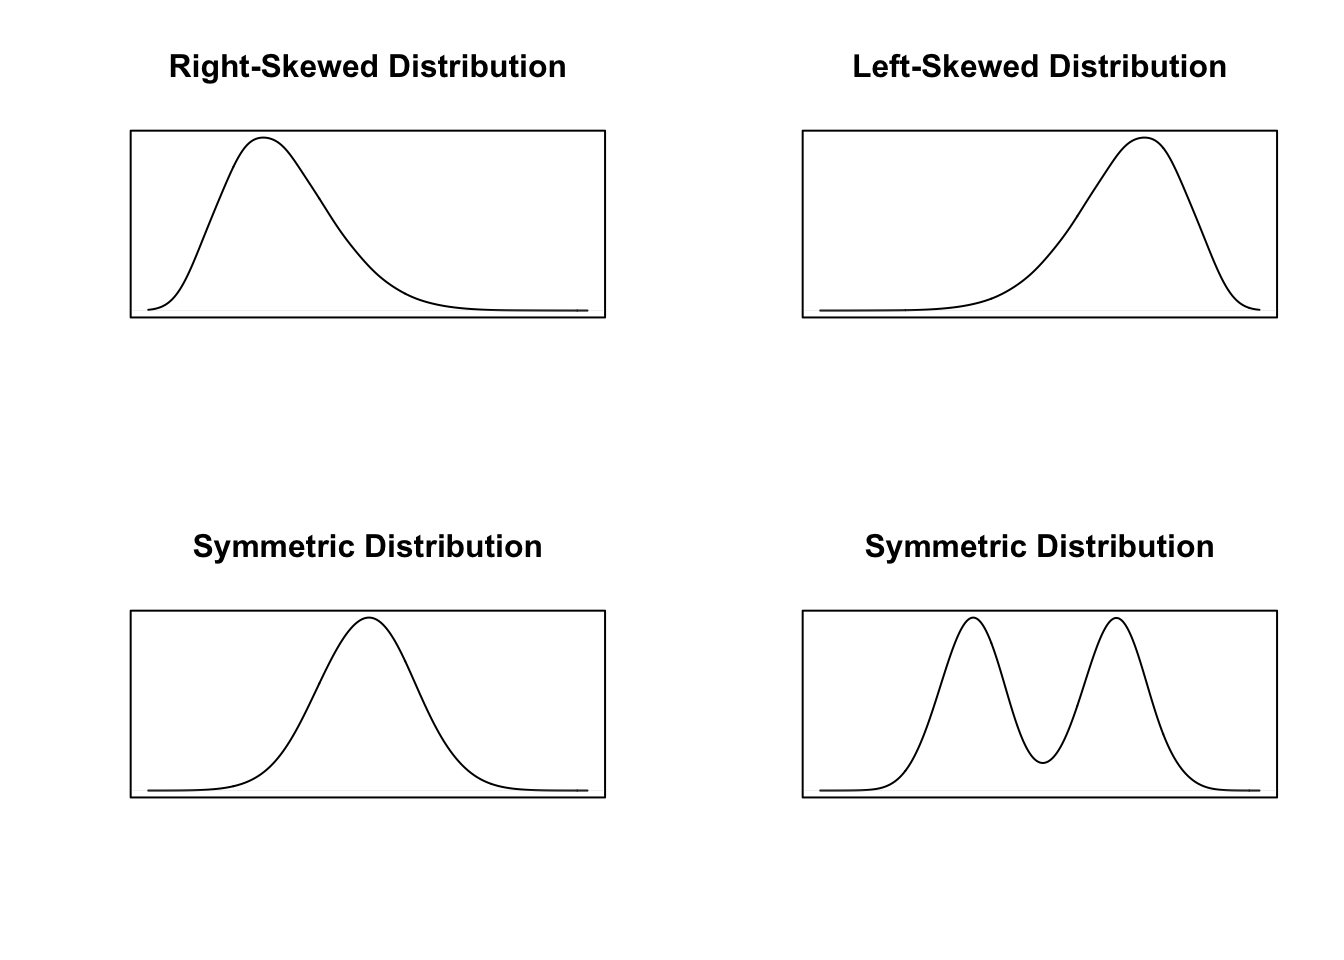
\includegraphics{IntroStats_files/figure-latex/unnamed-chunk-23-1.pdf}

Notice that the bottom left plot comes to a sharper peak, while the bottom right has a gentler slope. This is what we mean by ``spread'': the density on the bottom right is the most spread out.

To check whether a variable is (approximately) normally distributed,

\begin{enumerate}
\def\labelenumi{\arabic{enumi}.}
\tightlist
\item
  Check the histogram to see if it is symmetric and bell-shaped.
\item
  Estimate the parameters: \(\mu\) using \(\bar{x}\) and \(\sigma\) using \(s\).
\end{enumerate}

\hypertarget{the-standard-normal-distribution}{%
\subsection{The Standard Normal Distribution}\label{the-standard-normal-distribution}}

In order to make normal distributions easier to work with, we will \textbf{standardize} them. A \textbf{standard normal distribution} is a normal distribution with mean \(\mu=0\) and standard deviation \(\sigma=1\). We standardize a variable using \[z = \frac{x-\mu}{\sigma}.\] This is also called a \textbf{z-score}. Standardizing using this formula will \emph{always} result in a variable with mean 0 and standard deviation 1 (even if it's not normal!). If \(X\) is approximately normal, then the standardized variable \(Z\) will have a standard normal distribution.

Note: when we z-score a variable, we preserve the area under the curve properties! If \(X\) is Normal\((\mu,\sigma)\), then \[P(X < c) = P\left(Z < \frac{c - \mu}{\sigma}\right) = P(Z < z).\]

\hypertarget{area-under-the-standard-normal-curve}{%
\section{Area Under the Standard Normal Curve}\label{area-under-the-standard-normal-curve}}

Properties:

\begin{enumerate}
\def\labelenumi{\arabic{enumi}.}
\tightlist
\item
  Total area under the curve is 1.
\item
  The curve extends infinitely in both directions, never touching the horizontal axis.
\item
  Symmetric about 0.
\item
  Almost all of the area under the curve is between -3 and 3.
\end{enumerate}

We will think about area under the standard normal curve in terms of \textbf{cumulative probabilities} or probabilities of the form \(P(Z < z)\).

We will use the fact that the total area under the curve is 1 to find probabilities like \(P(Z > c)\):

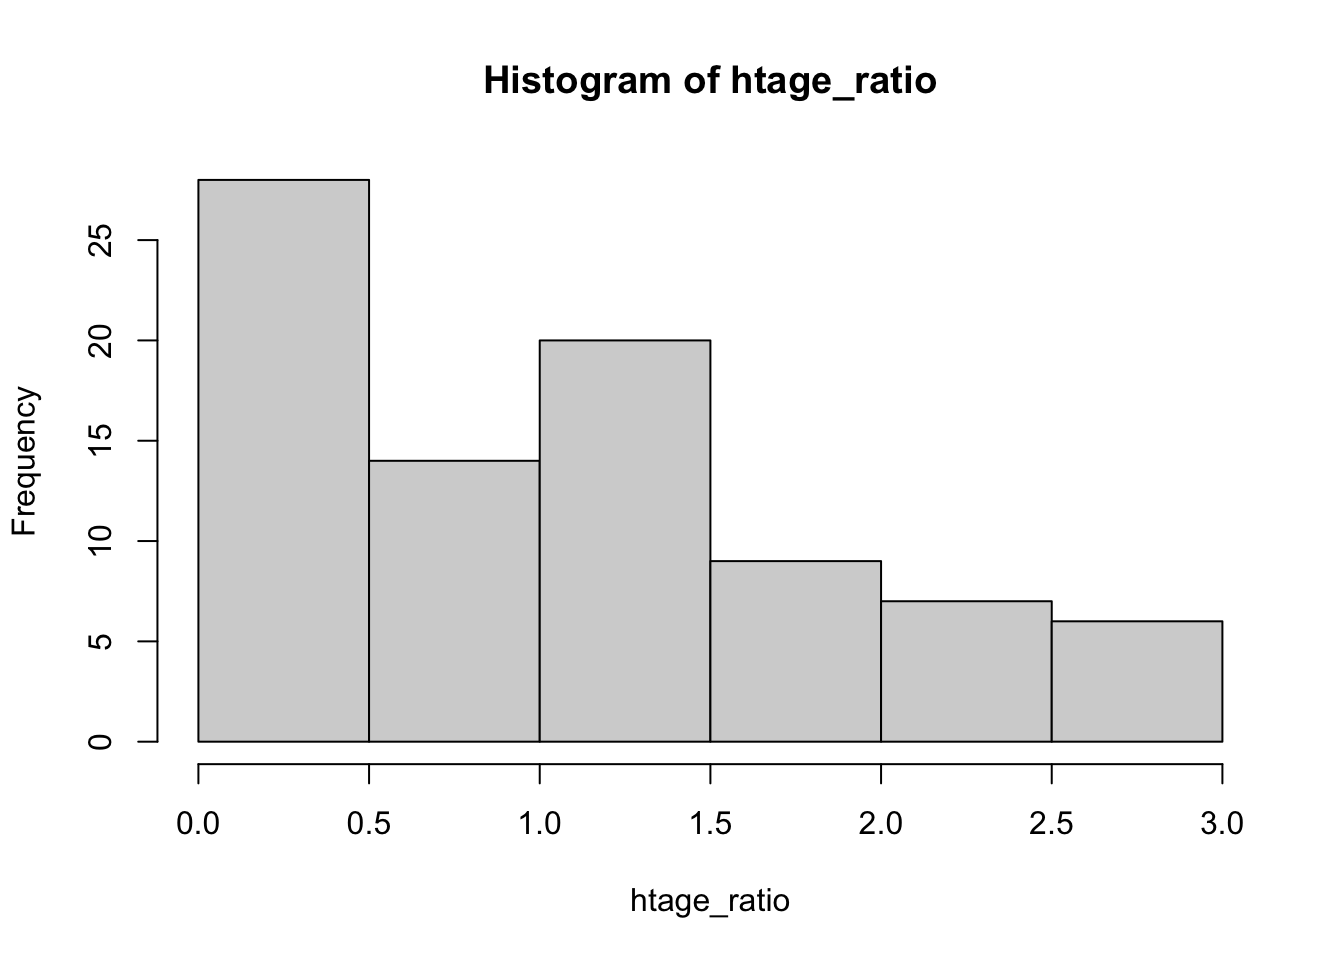
\includegraphics{IntroStats_files/figure-latex/unnamed-chunk-24-1.pdf}

Using the graphic to help visualize, we can see that \[1 = P(Z < c) + P(Z > c)\] which we can then rewrite as
\[P(Z > c) = 1-P(Z<c).\]

We can also use this concept to find \(P(a < Z < b)\).

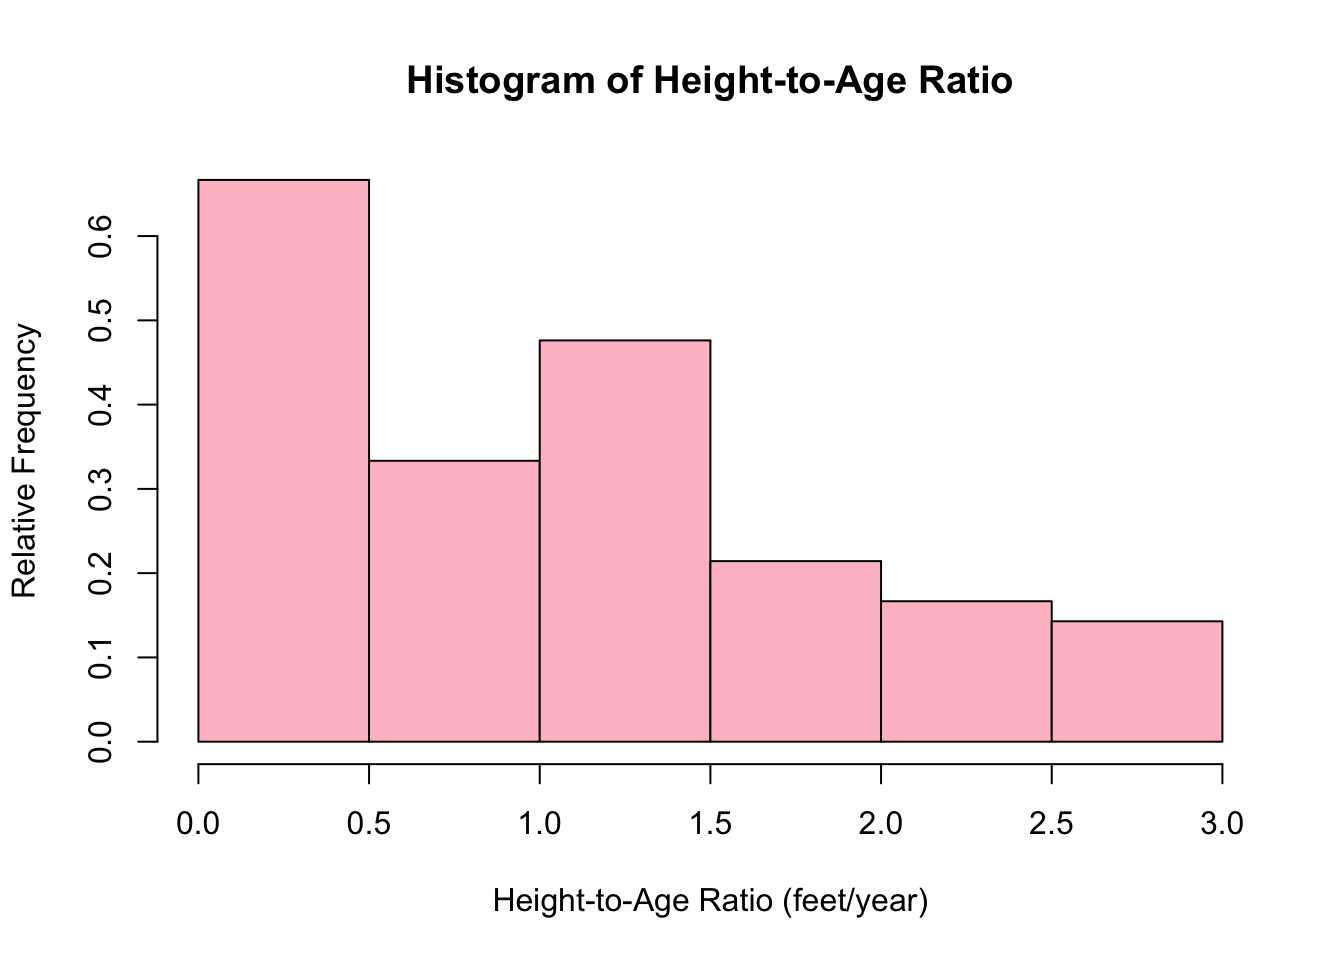
\includegraphics{IntroStats_files/figure-latex/unnamed-chunk-25-1.pdf}

Notice that \[1 = P(Z < a) + P(a < Z < b) + P(Z > b),\] which we can rewrite as \[P(a < Z < b) = 1 - P(Z > b) - P(Z < a)\] and since we just found that \(P(Z > b) = 1 - P(Z < b)\), we can replace \(1 - P(Z > b)\) with \(P(Z < b)\), and get \[P(a < Z < b) = P(Z < b) - P(Z < a).\]

\textbf{Key Cumulative Probability Concepts}

\begin{itemize}
\tightlist
\item
  \(P(Z > c) = 1 - P(Z < c)\)
\item
  \(P(a < Z < b) = P(Z < b) - P(Z < a)\)
\end{itemize}

A final note, because the normal distribution is symmetric, \(P(X < \mu) = P(X > \mu) = 0.5\). Notice this also implies that, when a distribution is symmetric (and unimodal), the mean and median are the same!

Now that we can get all of our probabilities written as \emph{cumulative} probabilities, we're ready to use software to find the area under the curve!

\textbf{Finding Area Under the Curve: R}

We will use statistical software called \texttt{R} to find areas under the curve. R is an incredibly powerful statistical programming language, but we're going to keep it simple. \(P(Z < z)\) is found using the command `pnorm(z)'. To find \(P(Z<1)\), I would type \texttt{pnorm(1)}. That entry and \texttt{R} output look like this:

\begin{Shaded}
\begin{Highlighting}[]
\FunctionTok{pnorm}\NormalTok{(}\DecValTok{1}\NormalTok{)}
\end{Highlighting}
\end{Shaded}

\begin{verbatim}
## [1] 0.8413447
\end{verbatim}

so \(P(Z < 1) = 0.8413447\). Since we are only going to use R for a few simple commands, we will run it completely online at the website rdrr.io/snippets (bookmark this website!)

For now, you can run R right here in the course notes! This is exactly what you will see on the rdrr.io website. Type in your command and click the green ``Run'' button. Try finding \(P(Z < 2)\).

Make sure you are able to run the command and get \(P(Z<2)=0.9772499\). (If it prints out ``Sorry, something went wrong. All I know is:'', just press the ``Run'' button again.)

We can also find a z-score given a specified area/probability. The notation \(z_{\alpha}\) (z-alpha) is the z-score corresponding to a right-tail area of \(\alpha\). That is, \[P(Z>z_{\alpha}) = \alpha\] We can find \(z_{\alpha}\) using the command \texttt{qnorm(p,\ lower.tail=FALSE)}. To find \(P(Z>z_{\alpha}) = 0.1\), I would type

\begin{Shaded}
\begin{Highlighting}[]
\FunctionTok{qnorm}\NormalTok{(}\FloatTok{0.1}\NormalTok{, }\AttributeTok{lower.tail=}\ConstantTok{FALSE}\NormalTok{)}
\end{Highlighting}
\end{Shaded}

\begin{verbatim}
## [1] 1.281552
\end{verbatim}

so if \(P(Z>z_{\alpha}) = 0.1\), then \(z_{\alpha}=1.281552\). (If you wanted to consider \(P(Z < z) = p\), you would replace ``FALSE'' with ``TRUE''.)

A quick note about \texttt{R}: \texttt{R} will print very large numbers and numbers close to 0 using \emph{scientific notation}. However, \texttt{R}'s scientific notation may not look the way you're used to! Check out the \texttt{R} output for \(P(Z < -5)\):

\begin{Shaded}
\begin{Highlighting}[]
\FunctionTok{pnorm}\NormalTok{(}\SpecialCharTok{{-}}\DecValTok{5}\NormalTok{)}
\end{Highlighting}
\end{Shaded}

\begin{verbatim}
## [1] 2.866516e-07
\end{verbatim}

When you see \texttt{e-07}, that means \(\times10^{-7}\)\ldots{} so \(P(Z < -5) = 2.8665 \times 10^{-7} \approx 0.00000029\).

\textbf{Finding Area Under the Curve: Applets}

Another option for finding probabilities and z-scores associated with the normal curve is to use an online applet. The Rossman and Chance Normal Probability Calculator is my preferred applet. It's relatively straightforward to use and would be difficult to demonstrate in these course notes! We will demonstrate this applet in class. I recommend you bookmark any websites you use to find probabilities!

You can also find the area under a normal distribution using a Normal Distribution Table. These are outdated and not used anywhere but the statistics classroom. As a result, I do not teach them. However, if you wish to use the table instead of R, there is a short tutorial here.

\hypertarget{working-with-normally-distributed-variables}{%
\section{Working with Normally Distributed Variables}\label{working-with-normally-distributed-variables}}

\hypertarget{normal-distribution-probabilities}{%
\subsection{Normal Distribution Probabilities}\label{normal-distribution-probabilities}}

Using z-scores and area under the standard normal curve, we can find probabilities for any normal distribution problem!

\textbf{Determining Normal Distribution Probabilities}

\begin{enumerate}
\def\labelenumi{\arabic{enumi}.}
\tightlist
\item
  Sketch the normal curve for the variable.
\item
  Shade the region of interest and mark its delimiting x-value(s).
\item
  Find the z-score(s) for the value(s).
\item
  Use the \texttt{pnorm} command in \texttt{R} to find the associated area.
\end{enumerate}

\begin{quote}
\emph{Example}: Find the proportion of SAT-takers who score between 1150 and 1300. Assume that SAT scores are approximately normally distributed with mean \(\mu=1100\) and standard deviation \(\sigma = 200\).

First, let's figure out what we want to calculate. Using area under the curve concepts, the proportion of test-takers who score \emph{between} 1150 and 1300 will be \(P(1150 < X < 1300)\).

\begin{enumerate}
\def\labelenumi{\arabic{enumi}.}
\tightlist
\item
  Sketch:
\end{enumerate}
\end{quote}

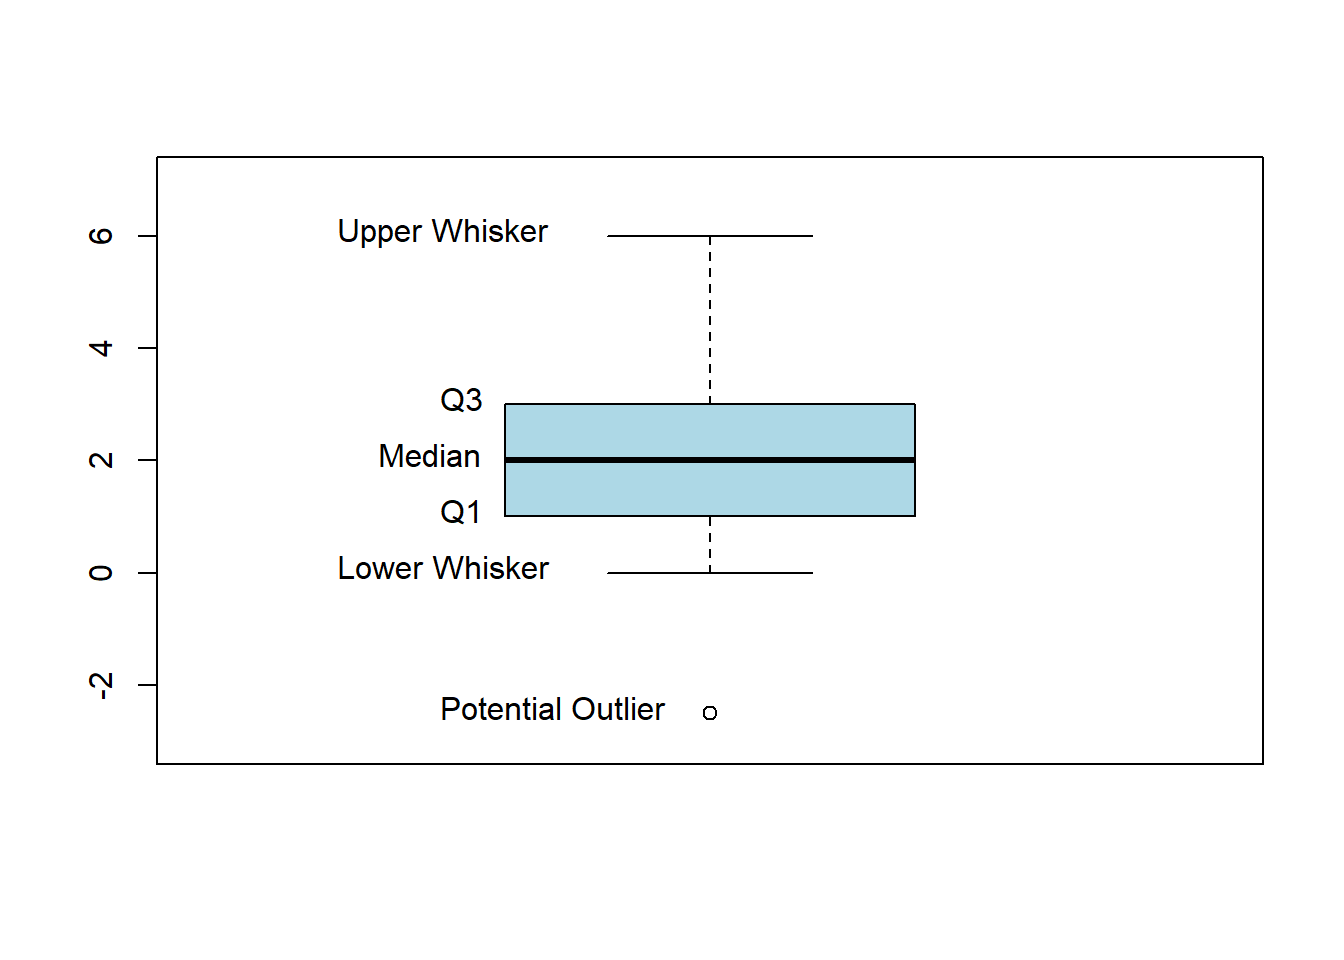
\includegraphics{IntroStats_files/figure-latex/unnamed-chunk-29-1.pdf}

\begin{quote}
\begin{enumerate}
\def\labelenumi{\arabic{enumi}.}
\setcounter{enumi}{1}
\tightlist
\item
  Shade and label:
\end{enumerate}
\end{quote}

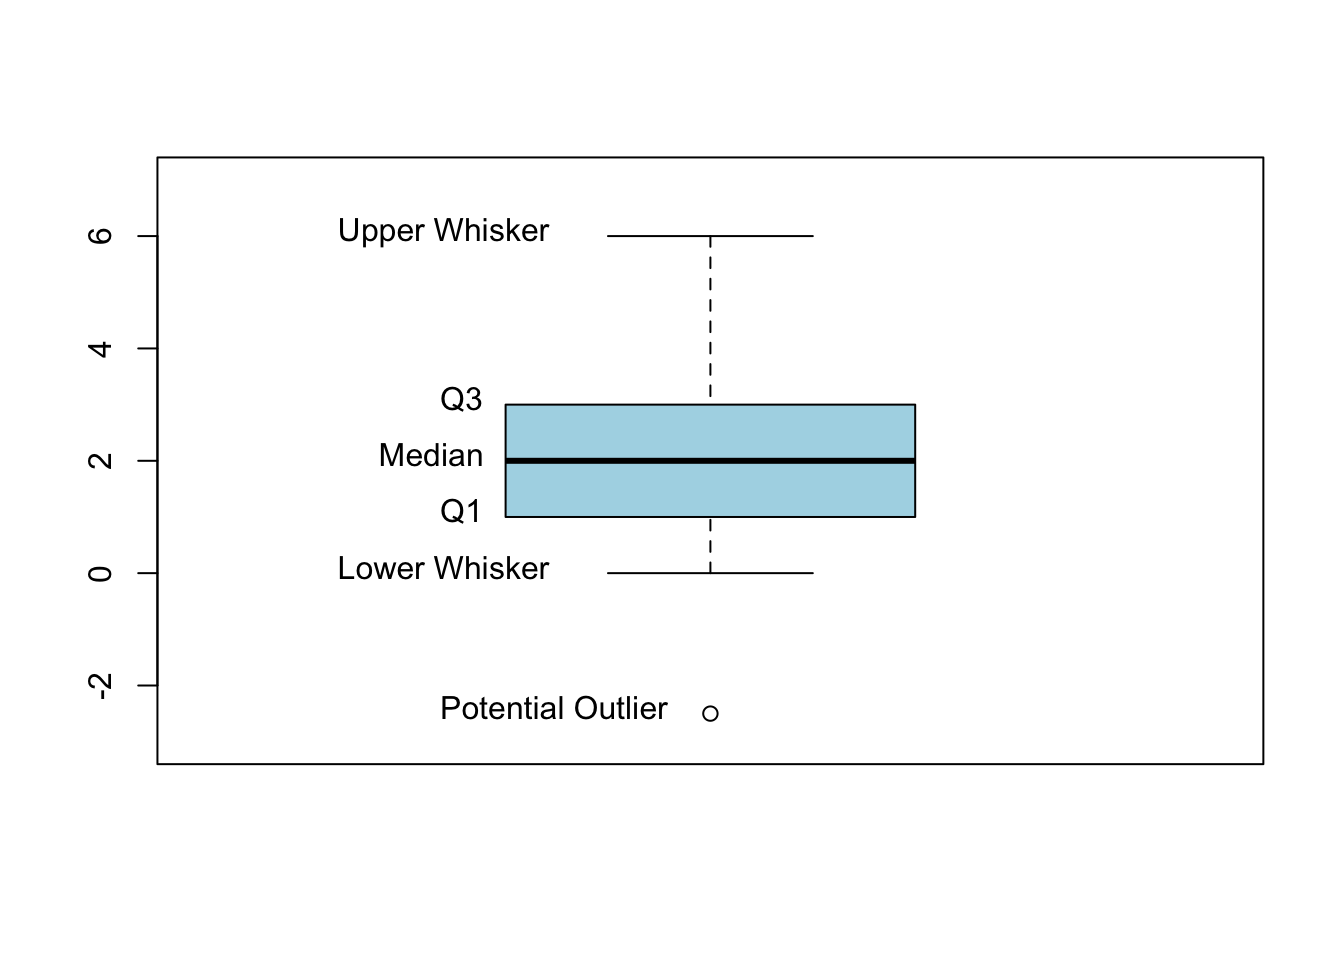
\includegraphics{IntroStats_files/figure-latex/unnamed-chunk-30-1.pdf}

\begin{quote}
\begin{enumerate}
\def\labelenumi{\arabic{enumi}.}
\setcounter{enumi}{2}
\tightlist
\item
  Calculate z-scores: \[x = 1150 \rightarrow z = \frac{1150-1100}{200} = 0.25\] and \[x=1300 \rightarrow z = \frac{1300-1100}{200} = 1.\]
\item
  Use \texttt{R} with \texttt{pnorm} to find \(P(Z < 0.25)\) and \(P(Z < 1)\):
\end{enumerate}
\end{quote}

\begin{Shaded}
\begin{Highlighting}[]
\FunctionTok{pnorm}\NormalTok{(}\FloatTok{0.25}\NormalTok{)}
\end{Highlighting}
\end{Shaded}

\begin{verbatim}
## [1] 0.5987063
\end{verbatim}

\begin{Shaded}
\begin{Highlighting}[]
\FunctionTok{pnorm}\NormalTok{(}\DecValTok{1}\NormalTok{)}
\end{Highlighting}
\end{Shaded}

\begin{verbatim}
## [1] 0.8413447
\end{verbatim}

\begin{quote}
Note that \[P(1150 < X < 1300) = P\left(\frac{1150-1100}{200} < Z < \frac{1300-1100}{200}\right) = P(0.25 < Z < 1)\] and, using cumulative probability concepts, \[P(0.25 < Z < 1) = P(Z < 1) - P(Z < 0.25).\] Using \texttt{R}, we found \(P(Z < 0.25) \approx 0.5987\) and \(P(Z < 1) \approx 0.8413\), so \[P(Z < 1) - P(Z < 0.25) \approx 0.8413 - 0.5987 = 0.2426.\] That is, approximately 26.26\% of test-takers score between 1150 and 1300 on the SAT.
\end{quote}

\hypertarget{empirical-rule-for-variables}{%
\subsection{Empirical Rule for Variables}\label{empirical-rule-for-variables}}

For any (approximately) normally distributed variable,

\begin{enumerate}
\def\labelenumi{\arabic{enumi}.}
\tightlist
\item
  Approximately 68\% of all possible observations lie within one standard deviation of the mean: \(\mu \pm \sigma.\)
\item
  Approximately 95\% of all possible observations lie within two standard deviations of the mean: \(\mu \pm 2\sigma.\)
\item
  Approximately 99.7\% of all possible observations lie within three standard deviations of the mean: \(\mu \pm 3\sigma.\)
\end{enumerate}

Given some data, you can check if approximately 68\% of the data falls within \(\bar{x}\pm s\), 95\% within \(\bar{x}\pm 2s\), and 99.7\% within \(\bar{x}\pm 3s\) to examine whether the data follow the empirical rule.

Note that a z-score tells us how many standard deviations an observation is from the mean. A positive z-score \(z>0\) is \emph{above} the mean; a negative z-score \(z<0\) is \emph{below} the mean.

\begin{quote}
\emph{Example}: \(z=-0.23\) is 0.23 standard deviations below the mean.
\end{quote}

\hypertarget{percentiles}{%
\subsection{Percentiles}\label{percentiles}}

We can also find the \emph{observation} associated with a percentage/proportion.

The \(w\)th \textbf{percentile} \(p_w\) is the observation that is higher than w\% of all observations \[P(X < p_w) = w\]

\textbf{Finding a Percentile}

\begin{enumerate}
\def\labelenumi{\arabic{enumi}.}
\tightlist
\item
  Sketch the normal curve for the variable.
\item
  Shade the region of interest and label the area.
\item
  Use the applet to determine the z-score for the area.
\item
  Find the x-value using \(z\), \(\mu\), and \(\sigma\).
\end{enumerate}

Note that if \(z = \frac{x-\mu}{\sigma}\), then \(x = \mu + z\sigma\).

\begin{quote}
\emph{Example}: Find the 90th percentile for SAT scores.

From the previous example, we know that SAT scores are approximately Normal(\(\mu=1100\), \(\sigma=200\)).
1. Sketch the normal curve.
\end{quote}

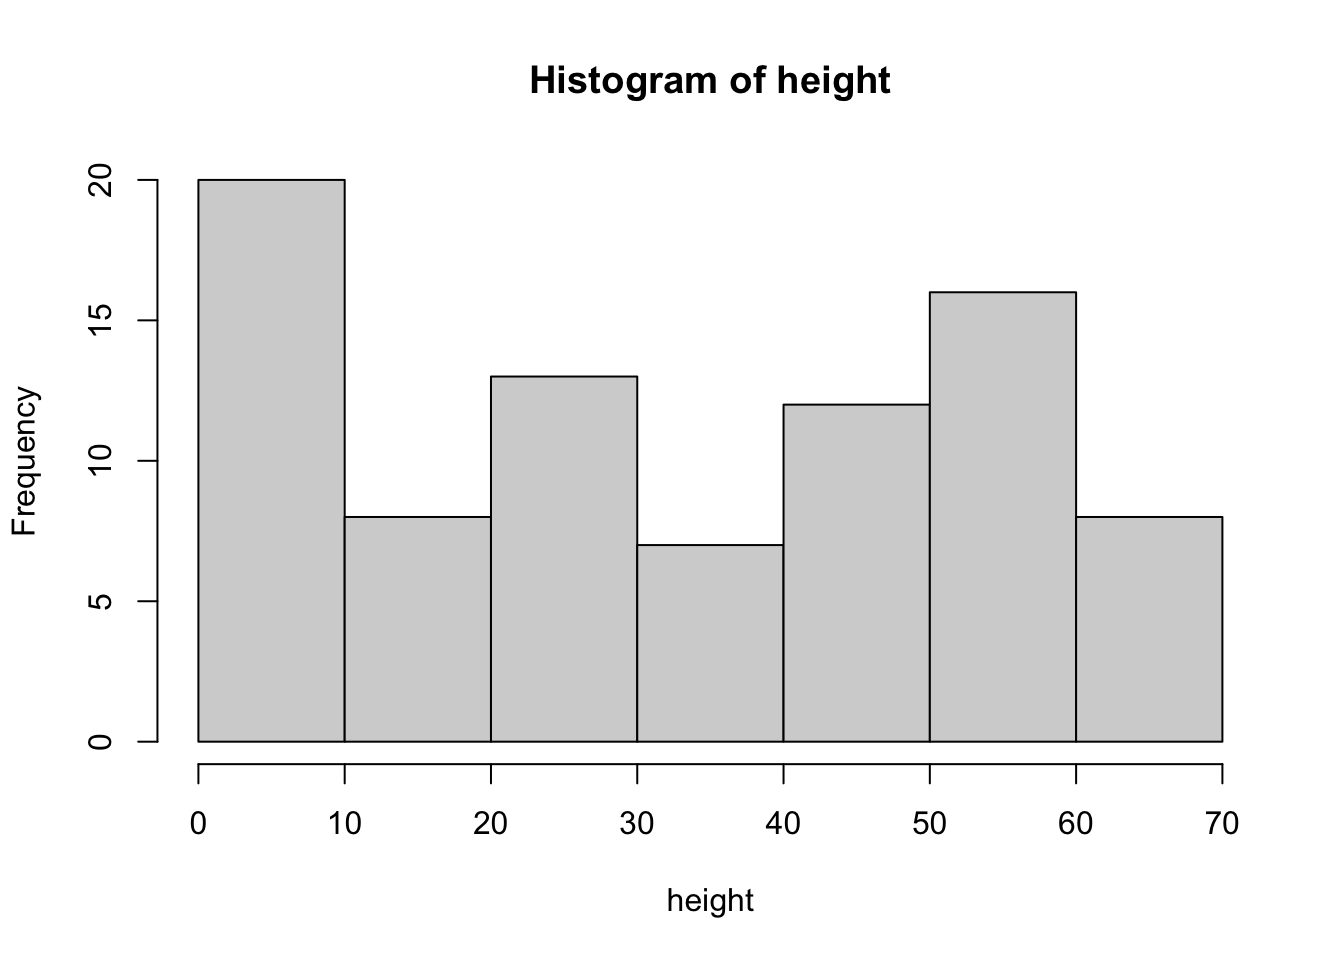
\includegraphics{IntroStats_files/figure-latex/unnamed-chunk-32-1.pdf}

\begin{quote}
\begin{enumerate}
\def\labelenumi{\arabic{enumi}.}
\setcounter{enumi}{1}
\tightlist
\item
  Shade the region of interest and label the area.
\end{enumerate}
\end{quote}

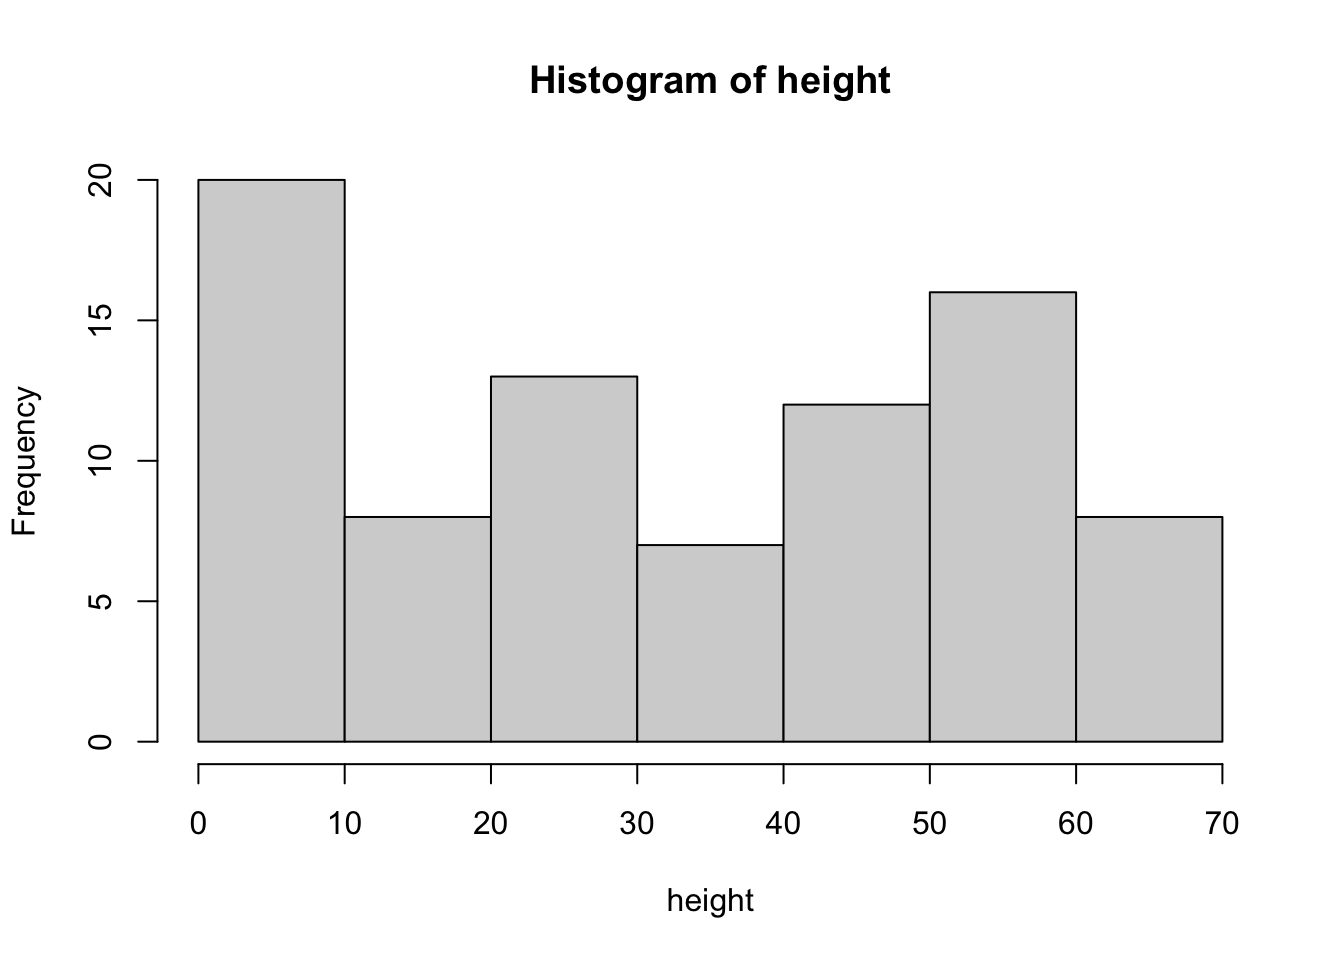
\includegraphics{IntroStats_files/figure-latex/unnamed-chunk-33-1.pdf}

\begin{quote}
\begin{enumerate}
\def\labelenumi{\arabic{enumi}.}
\setcounter{enumi}{2}
\tightlist
\item
  Use \texttt{R} with \texttt{qnorm} to determine the z-score for the area:
\end{enumerate}
\end{quote}

\begin{Shaded}
\begin{Highlighting}[]
\FunctionTok{qnorm}\NormalTok{(}\FloatTok{0.9}\NormalTok{)}
\end{Highlighting}
\end{Shaded}

\begin{verbatim}
## [1] 1.281552
\end{verbatim}

\begin{quote}
Find the x-value using \(z\approx 1.2816\), \(\mu=1100\), and \(\sigma=200\): \[x = 1100 + 1.2816(200) = 1356.32\] so 90\% of SAT test-takers score below 1356.32.
\end{quote}

\hypertarget{introduction-to-inference}{%
\chapter{Introduction to Inference}\label{introduction-to-inference}}

\hypertarget{module-overview-4}{%
\section{Module Overview}\label{module-overview-4}}

This module will bridge the gap between our discussion on the normal distribution and our first forays into statistical inference. As it turns out, much of the statistical inference we will use relies on the normal distribution and the t-distribution, which we will introduce in this module. We begin our study of statistical inference by learning about confidence intervals.

\textbf{Module Learning Objectives/Outcomes}

\begin{enumerate}
\def\labelenumi{\arabic{enumi}.}
\tightlist
\item
  Find the distribution of a sample mean.
\item
  Estimate probabilities for a sample mean.
\item
  Calculate and interpret confidence intervals for a population mean.
\item
  Use the standard normal and t-distributions to find critical values.
\end{enumerate}

This module's outcomes correspond to course outcome (6) apply statistical inference techniques of parameter estimation such as point estimation and confidence interval estimation and (7) apply techniques of testing various statistical hypotheses concerning population parameters.

\hypertarget{sampling-distributions}{%
\section{Sampling Distributions}\label{sampling-distributions}}

\hypertarget{sampling-error}{%
\subsection{Sampling Error}\label{sampling-error}}

We want to use a sample to learn something about a population, but no sample is perfect! \textbf{Sampling error} is the error resulting from using a sample to estimate a population characteristic.

If we use a sample mean \(\bar{x}\) to estimate \(\mu\), chances are that \(\bar{x}\ne\mu\) (they might be close but\ldots{} they might not be!). We will consider

\begin{itemize}
\tightlist
\item
  How close \emph{is} \(\bar{x}\) to \(\mu\)?
\item
  What if we took many samples and calculated \(\bar{x}\) many times?

  \begin{itemize}
  \tightlist
  \item
    How would that relate to \(\mu\)?
  \item
    What would be the distribution of these values?
  \end{itemize}
\end{itemize}

The distribution of a statistic (across all possible samples of size \(n\)) is called the \textbf{sampling distribution}. We will focus primarily on the distribution of the sample mean.

For a variable \(x\) and given a sample size \(n\), the distribution of \(\bar{x}\) is alled the \textbf{sampling distribution of the sample mean} or the \textbf{distribution of \(\boldsymbol{\bar{x}}\)}.

\begin{quote}
\emph{Example}: Suppose our population is the five starting players on a particular basketball team. We are interested in their heights (measures in inches). The full population data is

\begin{longtable}[]{@{}lccccc@{}}
\toprule
Player & A & B & C & D & E \\
\midrule
\endhead
Height & 76 & 78 & 79 & 81 & 86 \\
\bottomrule
\end{longtable}

The population mean is \(\mu=80\). Consider all possible samples of size \(n=2\):

\begin{longtable}[]{@{}lcccccccccc@{}}
\toprule
Sample & A,B & A,C & A,D & A,E & B,C & B,D & B,E & C,D & C,E & D,E \\
\midrule
\endhead
\(\bar{x}\) & 77 & 77.5 & 78.5 & 81.0 & 78.5 & 79.5 & 82.0 & 80.0 & 82.5 & 83.5 \\
\bottomrule
\end{longtable}

There are 10 possible samples of size 2. Of these samples, 10\% have means exactly equal to \(\mu\) (for a \emph{random} sample of size 2, you'd have a 10\% chance to find \(\bar{x}=\mu\)\ldots{} and a 90\% chance not to!).
\end{quote}

In general, the larger the sample size, the smaller the sampling error tends to be in estimating \(\mu\) using \(\bar{x}\).

In practice, we have one sample and \(\mu\) is unknown. We also have limited resources to collect data, so it may not be feasible to collect a very large sample.

The mean of the distribution of \(\bar{x}\) is \(\mu_{\bar{X}}=\mu\) and the standard deviation is \(\sigma_{\bar{X}}=\sigma/\sqrt{n}\). We refer to the standard deviation of a sampling distribution as \textbf{standard error}. (Note that this standard error formula is built for very large populations, so it will not work well for our basketball players. This is okay! We usually work with populations so large that we treat them as ``infinite''.)

\begin{quote}
\emph{Example}: The mean living space for a detatched single family home in the United States is 1742 ft\(^2\) with a standard deviation of 568 square feet. (Does that mean seem huge to anyone else??) For samples of 25 homes, determine the mean and standard error of \(\bar{x}\).

Using our formulae: \[\mu_{\bar{X}} = \mu = 1742\] and \[\sigma_{\bar{X}} = \frac{\sigma}{\sqrt{n}} = \frac{568}{\sqrt{25}} = 113.6.\]
\end{quote}

\hypertarget{the-sampling-distribution-of-barx}{%
\subsection{\texorpdfstring{The Sampling Distribution of \(\bar{X}\)}{The Sampling Distribution of \textbackslash bar\{X\}}}\label{the-sampling-distribution-of-barx}}

First, we consider the setting where \(X\) is Normal(\(\mu\), \(\sigma\)). The plots below show (A) a random sample of 1000 from a Normal(100, 25) distribution and (B) the approximate sampling distribution of \(\bar{X}\) when X is Normal(100, 25).

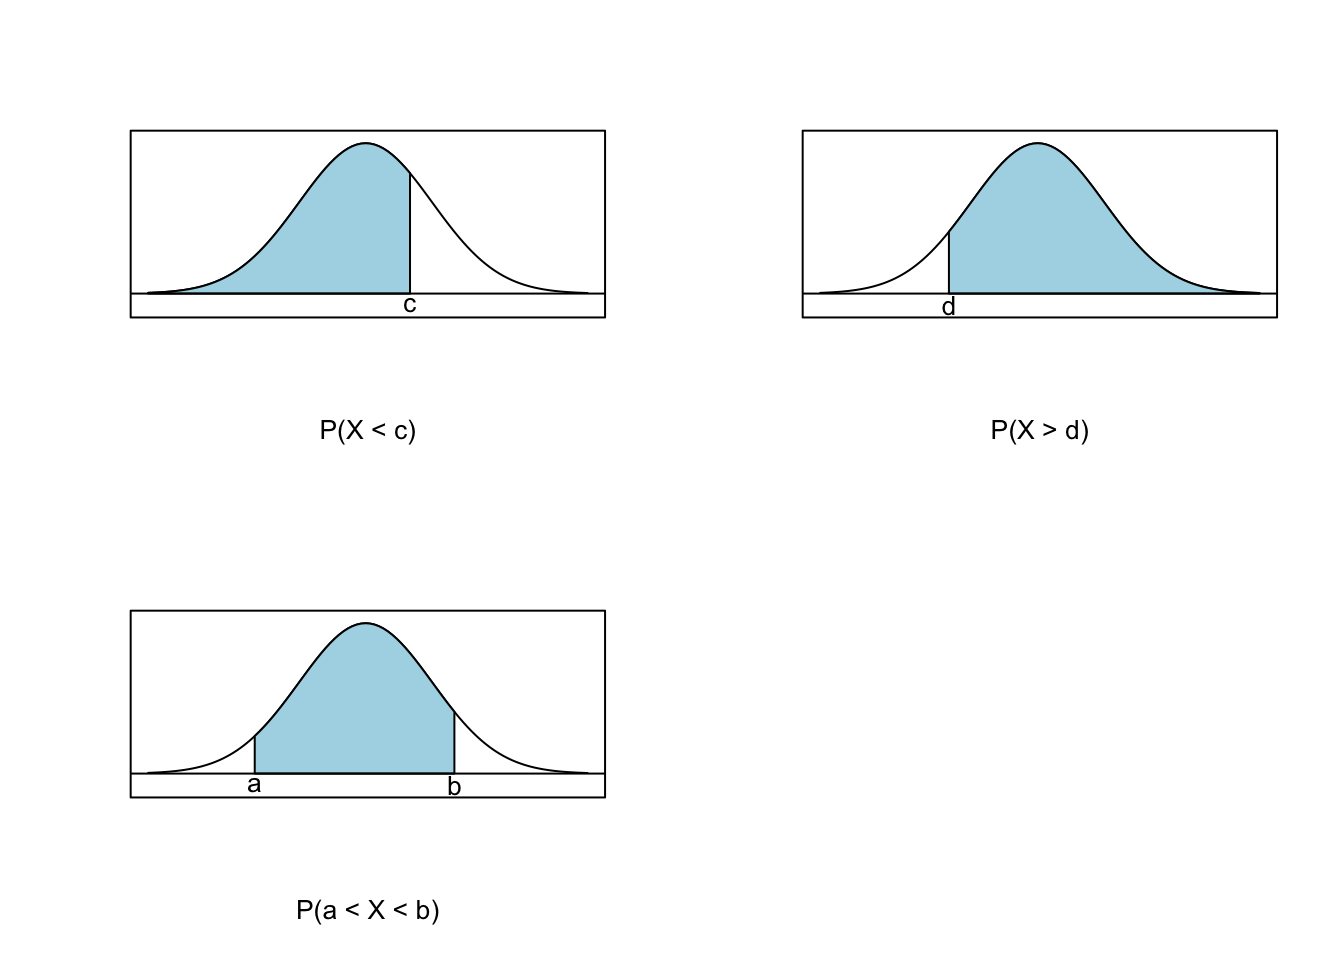
\includegraphics{IntroStats_files/figure-latex/unnamed-chunk-35-1.pdf}

Notice how the x-axis changes from one plot to the next.

In fact, if \(X\) is Normal(\(\mu\), \(\sigma\)), then \(\bar{X}\) is Normal(\(\mu_{\bar{X}}=\mu\), \(\sigma_{\bar{X}}=\sigma/\sqrt{n}\)).

\textbf{Central Limit Theorem}

For relatively large sample sizes, the random variable \(\bar{X}\) is approximately normally distributed \emph{regardless of the distribution of} \(X\): \[\bar{X}\text{ is Normal}(\mu_{\bar{X}}=\mu, \sigma_{\bar{X}}=\sigma/\sqrt{n}).\]

Notes

\begin{itemize}
\tightlist
\item
  This approximation improves with increasing sample size.
\item
  In general, ``relatively large'' means sample sizes \(n \ge 30\).
\end{itemize}

\hypertarget{developing-confidence-intervals}{%
\section{Developing Confidence Intervals}\label{developing-confidence-intervals}}

Recall: A \textbf{point estimate} is a single-value estimate of a population parameter. We say that a statistic is an \textbf{unbiased estimator} if the mean of its distribution is equal to the population parameter. Otherwise, it is a \textbf{biased estimator}.

\emph{Comment} Remember how our formula for standard deviation, the ``mean squared deviance'' divides by \(n-1\) instead of \(n\)? We do this so that \(s\) is an \emph{unbiased} estimate of \(\sigma\).

Ideally, we want estimates that are unbiased with small standard error. For example, a sample mean (unbiased) with a large sample size (results in smaller standard error).

Point estimates are useful, but they only give us so much information. The variability of an estimate is also important!

\begin{quote}
\emph{Example} Think about estimating what tomorrow's weather will be like. If it's May in Sacramento, the average high temperature is 82 degrees Fahrenheit, but it's not uncommon to have highs anywhere from 75 to 90! Since the highs are so \emph{variable}, it's hard to be confident using 82 to predict tomorrow's weather.

On the flip side, think about July in Phoenix. The average high is 106 degrees Fahrenheit. In Phoenix, it's uncommon to have a July day with a high below 100. Since the highs are \emph{not variable}, you could feel pretty confidence using 105 to predict tomorrow's weather.
\end{quote}

Take a look at these two boxplots:

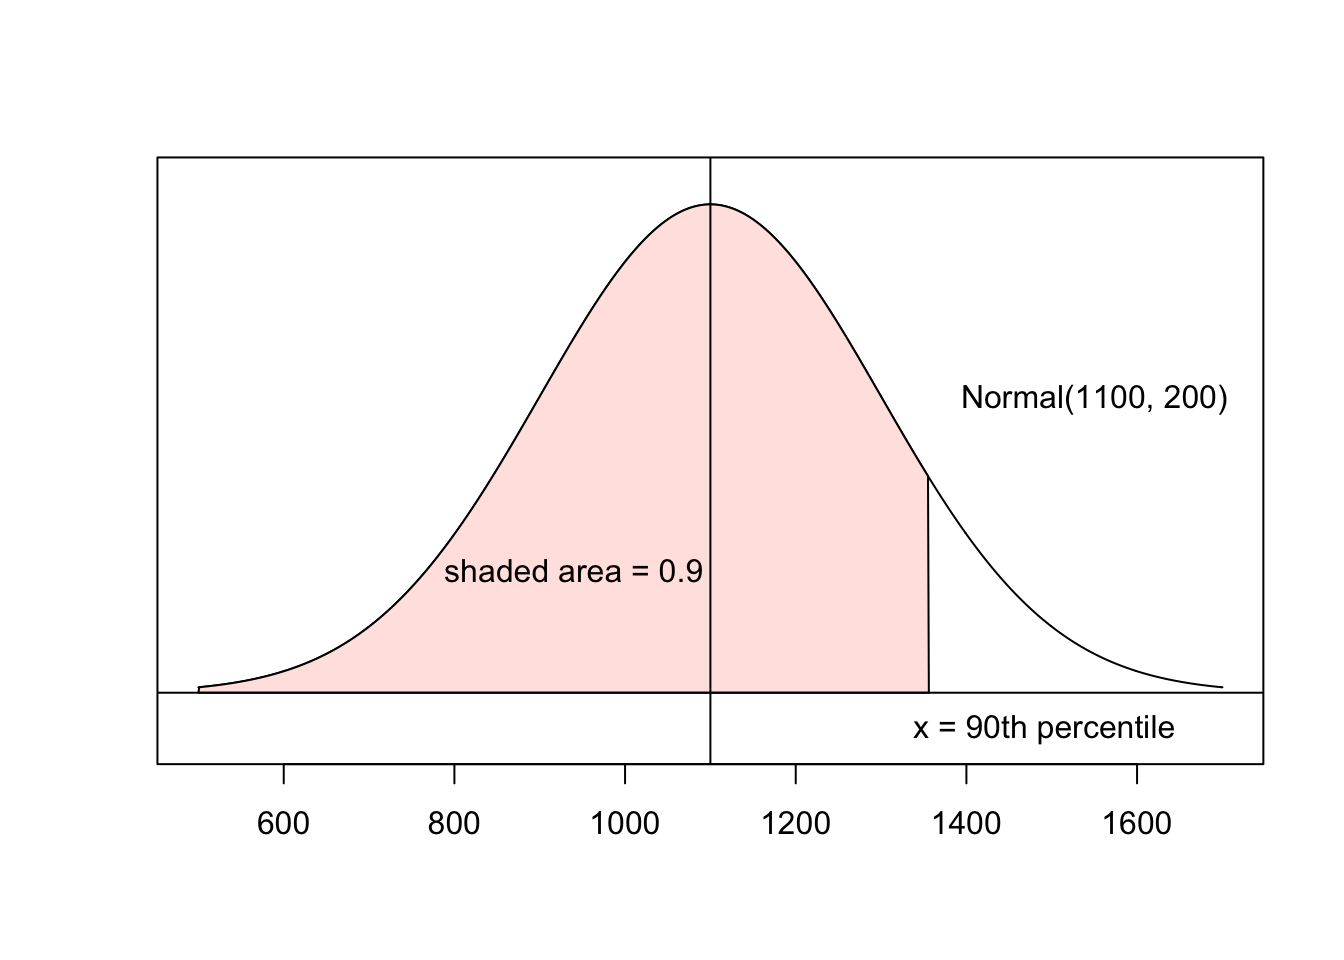
\includegraphics{IntroStats_files/figure-latex/unnamed-chunk-36-1.pdf}

Both samples are size \(n=100\) and have \(\bar{x}=0\), which would be our point estimate for \(\mu\)\ldots{} but Variable 1 has a standard deviation of \(\sigma=0.5\) and Variable 2 has standard deviation \(\sigma=5\). As a result, we can be more confident in our estimate of the population mean for Variable 1 than for Variable 2.

We want to formalize this idea of confidence in our estimates. A \textbf{confidence interval} is an interval of numbers based on the point estimate of the parameter. Say we want to be 95\% confident about a statement. In Statistics, this means that we have arrived at our statement using a method that will give us a correct statement 95\% of the time.

Assume we are taking a sample from a normal distribution with mean \(\mu\) and standard deviation \(\sigma\). We will assume the value of \(\sigma\) is known to us. Then \(\bar{X}\) is Normal(\(\mu, \sigma/\sqrt{n}\)). If we standardize \(\bar{X}\), we get \[Z = \frac{\bar{X}-\mu}{\sigma/\sqrt{n}}.\]

We want some interval \((a,b)\). We will start by considering \(a < Z < b\), so \(a < Z\) and \(Z < b\) (or \(b > Z\)). Then

\[
\begin{aligned}
Z &< b\\
\frac{\bar{X}-\mu}{\sigma/\sqrt{n}} &< b\\
\bar{X}-\mu &< b\sigma/\sqrt{n} \\
\bar{X}-b\sigma/\sqrt{n} &< \mu 
\end{aligned}
\]

and

\[
\begin{aligned}
a &< Z  \\
a &< \frac{\bar{X}-\mu}{\sigma/\sqrt{n}} \\
a\sigma/\sqrt{n} &< \bar{X}-\mu \\
\mu &< \bar{X}-a\sigma/\sqrt{n}
\end{aligned}
\]

putting these together, \[ \bar{X}-b\frac{\sigma}{\sqrt{n}} < \mu <  \bar{X}-a\frac{\sigma}{\sqrt{n}}.\] If we want to be 95\% confident, then we want \(P(a < Z < b)=0.95\): \[P\left(\bar{X}-b\frac{\sigma}{\sqrt{n}} < \mu <  \bar{X}-a\frac{\sigma}{\sqrt{n}}\right) = 0.95.\] To calculate the 95\% confidence interval, we need to find \(a\) and \(b\) such that \(P(a < Z < b)=0.95\).

We want this interval to be as narrow (small) as possible. Why? Narrower intervals are more informative. If I say I'm 95\% confidence that tomorrow's high will be between -100 and 200 degrees Fahrenheit, that's a useless interval. If I change it to between 70 and 100, that's a little better. Changing it to between 85 and 90 is even better. This is what we mean by more informative.

It turns out that, with a symmetric distribution like the normal distribution, the way to make a confidence interval as narrow as possible is to take advantage of this symmetry. Each of the plots below show a shaded area of 0.95. The narrowest interval (along the horizontal axis) is the first interval, which is shaded on \((-1.96 < z < 1.96)\).

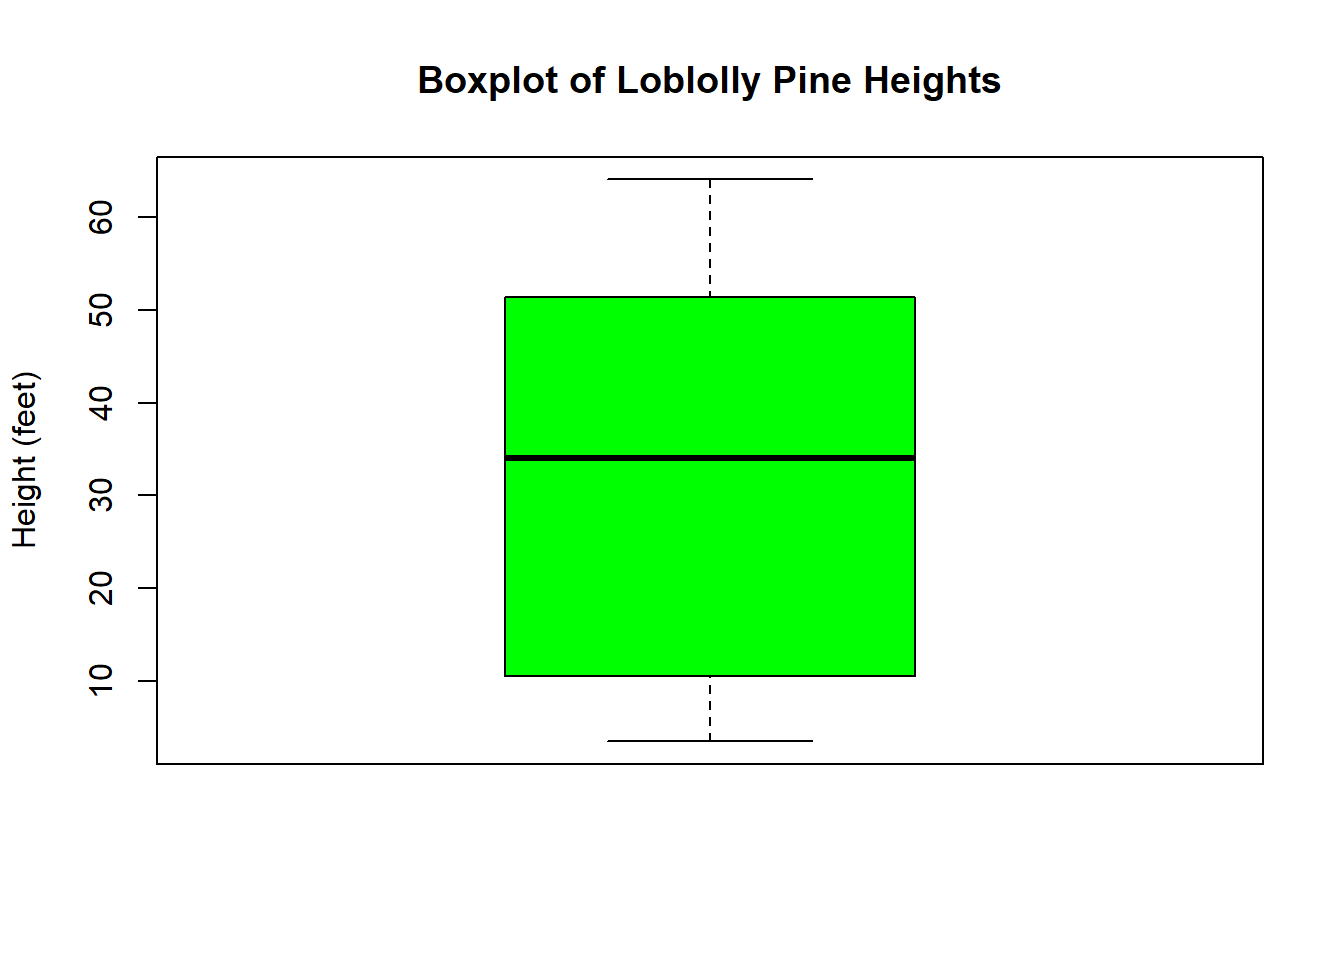
\includegraphics{IntroStats_files/figure-latex/unnamed-chunk-37-1.pdf}

The confidence interval, then, is \[\left(\bar{x} - z_*\frac{\sigma}{\sqrt{n}}, \bar{x} + z_*\frac{\sigma}{\sqrt{n}}\right)\] where \(z_* = 1.96\). The midpoint of this interval is \(\bar{x}\). The value of \[z_*\frac{\sigma}{\sqrt{n}}\] is called the \textbf{margin of error}.

\hypertarget{interpreting-a-confidence-interval}{%
\subsection{Interpreting a Confidence Interval}\label{interpreting-a-confidence-interval}}

To interpret a confidence interval, we need to think back to our definition of probability as ``the proportion of times is would occur if the experiment were run infinitely many times''. In the confidence interval case, if an experiment is run infinitely many times, the true value of \(\mu\) will be contained in 95\% of the intervals.

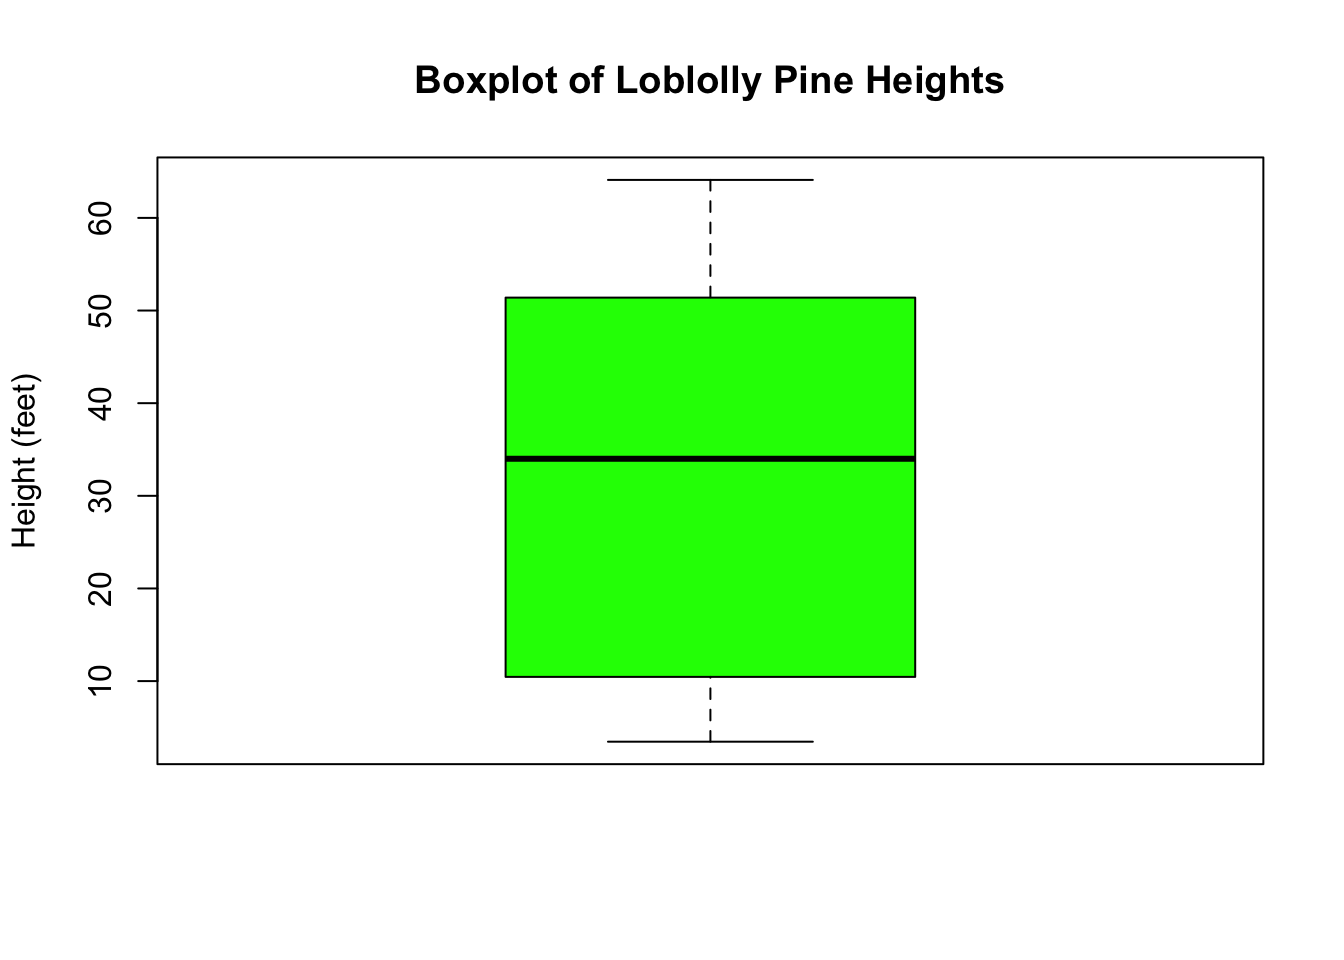
\includegraphics{IntroStats_files/figure-latex/unnamed-chunk-38-1.pdf}

The graphic above shows 95\% confidence intervals for 100 samples of size \(n=60\) drawn from a population with mean \(\mu=80\) and standard deviation \(\sigma=25\). Each sample's confidence interval is represented by a horizontal line. The dot in the middle of each is the sample mean. When a confidence interval does \emph{not} capture the population mean \(\mu\), the line is printed in red. Based on this concept of repeated sampling, we would expect about 95\% of these intervals to capture \(\mu\). In fact, 96 of the 100 intervals capture \(\mu\).

Finally, when you interpret a confidence interval, it is important to do so in the context of the problem.

\begin{quote}
\emph{Example} The preferred keyboard height for typists is approximately normally distributed with \(\sigma=2.0\). A sample of size \(n=31\), resulted in a mean prefered keyboard height of \(80 cm\). Find and interpret a 95\% confidence interval for keyboard height.

The interval is \[\bar{x} \pm z_{\alpha/2}\frac{\sigma}{\sqrt{n}} = 80.0 \pm 1.96\times\frac{2.0}{\sqrt{31}} = 80.0 \pm 0.70 = (79.3, 80.7).\] Interpretation:We can be 95\% confident that the mean preferred keyboard height for typists is between 79.3cm and 80.7cm.
\end{quote}

Notice that I kept the interpretation simple! That's okay - just be sure you are \emph{also} able to explain what it means to be 95\% confident (using the concept of repeated sampling).

Common mistakes:

\begin{itemize}
\tightlist
\item
  It is NOT accurate to say that ``the probability that \(\mu\) is in the confidence interval is 0.95''. The parameter \(\mu\) is some fixed quantity and it's either in the interval or it isn't.
\item
  We are NOT ``95\% confident that \(\bar{x}\) is in the interval''. The value \(\bar{x}\) is some known quantity and it's always in the interval.
\end{itemize}

\hypertarget{other-levels-of-confidence}{%
\section{Other Levels of Confidence}\label{other-levels-of-confidence}}

While the 95\% confidence interval is common in research, there's nothing inherently special about it. You could calculate a 90\%, a 99\%, or - if you're feeling spicy - something like a 43.8\% confidence interval. These numbers are called the \textbf{confidence level} and they represent the proportion of times that the parameter will fall in the interval (if we took many samples).

The 100(1-\(\alpha\))\% confidence interval for \(\mu\) is given by \[\bar{x}\pm z_{\alpha/2}\frac{\sigma}{\sqrt{n}}\] where \(z_{\alpha/2}\) is the \((\alpha/2)\)th percentile of the standard normal distribution. The value \(z_{\alpha/2}\) is called the \textbf{critical value} (``c.v.'' on the plot, below).

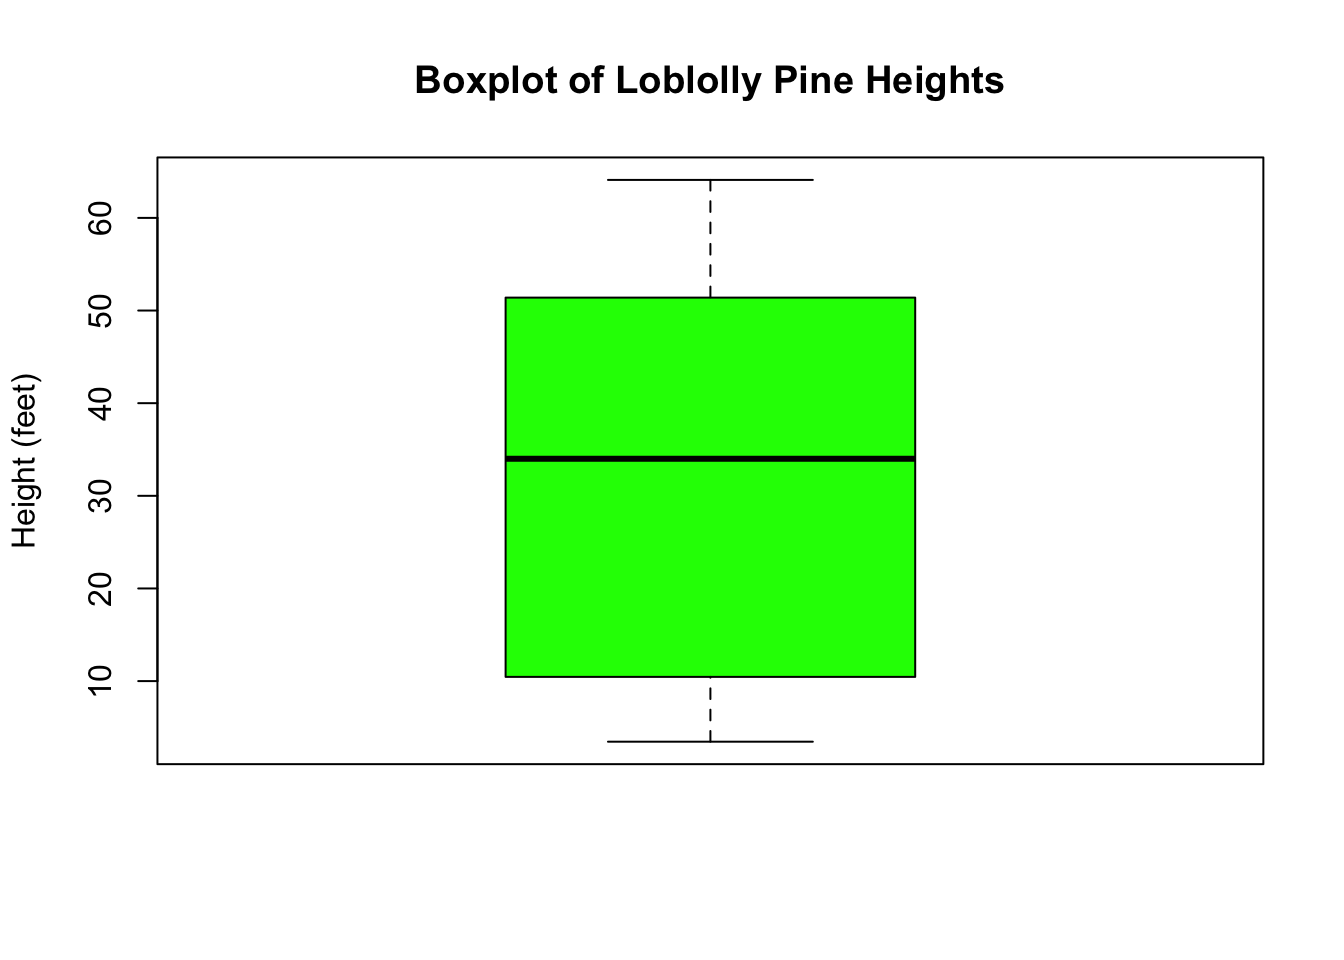
\includegraphics{IntroStats_files/figure-latex/unnamed-chunk-39-1.pdf}
We can find critical values in \texttt{R} using the same command we used to find percentiles: \texttt{qnorm(p)}. We want a 100(1-\(\alpha\)) confidence interval, so we need to quickly solve for \(\alpha\) and divide by 2. For example, for a 98\% interval, \[100(1-\alpha) = 98 \implies \alpha=0.02\] Then \(\alpha/2 = 0.01\) and

\begin{Shaded}
\begin{Highlighting}[]
\FunctionTok{qnorm}\NormalTok{(}\FloatTok{0.01}\NormalTok{)}
\end{Highlighting}
\end{Shaded}

\begin{verbatim}
## [1] -2.326348
\end{verbatim}

So the critical value is \(z_{\alpha/2}=2.326\). Notice that I dropped the negative sign here. That's because our formula uses \(\pm z_{\alpha/2}\), so the sign doesn't matter. I'll always ignore that negative for critical values. As long as you write your interval as \((\text{smaller number}, \text{bigger number})\), it's all good.

\textbf{Common Critical Values}

\begin{longtable}[]{@{}ccc@{}}
\toprule
Confidence Level & \(\alpha\) & Critical Value, \(z_{\alpha/2}\) \\
\midrule
\endhead
90\% & 0.10 & 1.645 \\
95\% & 0.05 & 1.90 \\
99\% & 0.01 & 2.575 \\
\bottomrule
\end{longtable}

\hypertarget{confidence-level-precision-and-sample-size}{%
\subsection{Confidence Level, Precision, and Sample Size}\label{confidence-level-precision-and-sample-size}}

If we can be 99\% confident (or even higher), why do we tend to ``settle'' for 95\%?? Take a look at the common critical values (above) and the confidence interval formula \[\bar{x} \pm z_{\alpha/2}\frac{\sigma}{\sqrt{n}}.\] What will higher levels of confidence do to this interval? Think back to the intuitive interval width explanation with the weather. Mathematically, the same thing will happen: the interval will get wider! And remember, a narrow interval is a more informative interval. There is a trade off here between interval width and confidence. In general, the scientific community has settled on 95\% as a compromise between the two, but different fields may use different levels of confidence.

There is one other thing we can control in the confidence interval: the sample size \(n\). One strategy is to specify the confidence level and the maximum acceptable interval width and use these to determine sample size. We know that \[\text{interval width}=2z_{\alpha/2}\frac{\sigma}{\sqrt{n}}\] Letting interval width equal \(w\), we can solve for \(n\): \[ n = \left(2z_{\alpha/2}\frac{\sigma}{w}\right)^2\] Alternately, we may specify a maximum margin of error \(m\) instead: \[ n = \left(z_{\alpha/2}\frac{\sigma}{m}\right)^2\]

A few comments:

\begin{itemize}
\tightlist
\item
  As desired width/margin of error decreases, \(n\) will increase.
\item
  As \(\sigma\) increases, \(n\) will also increase. (More population variability will necessitate a larger sample size.)
\item
  As confidence level increases, \(n\) will also increase.
\end{itemize}

\hypertarget{confidence-intervals-sigma-unknown}{%
\section{\texorpdfstring{Confidence Intervals, \(\sigma\) Unknown}{Confidence Intervals, \textbackslash sigma Unknown}}\label{confidence-intervals-sigma-unknown}}

In practice, the value of \(\sigma\) is almost never known\ldots{} but we know that we can estimate \(\sigma\) using \(s\). Can we plug in \(s\) for \(\sigma\)? Sometimes!

Remember the Central Limit Theorem (Section 5.1)? For samples of size \(n \ge 30\), \(\bar{X}\) will be approximately normal even if \(X\) isn't. In this case, we can plug in \(s\) for \(\sigma\): \[\bar{x} \pm z_{\alpha/2}\frac{s}{\sqrt{n}}.\]

Too easy? Okay, we do need to consider the setting where \(n < 30\), which will require a bit of additional work.

\hypertarget{the-t-distribution}{%
\subsection{The T-Distribution}\label{the-t-distribution}}

Enter: the t-distribution. If \[Z = \frac{\bar{Z}-\mu}{\sigma/\sqrt{n}}\] has a standard normal distribution, the slightly modified \[T = \frac{\bar{X}-\mu}{s/\sqrt{n}}\] has what we call the \textbf{t-distribution} with \(n-1\) \textbf{degrees of freedom}. The only thing we need to know about degrees of freedom is that \(df=n-1\) is the t-distribution's only parameter.

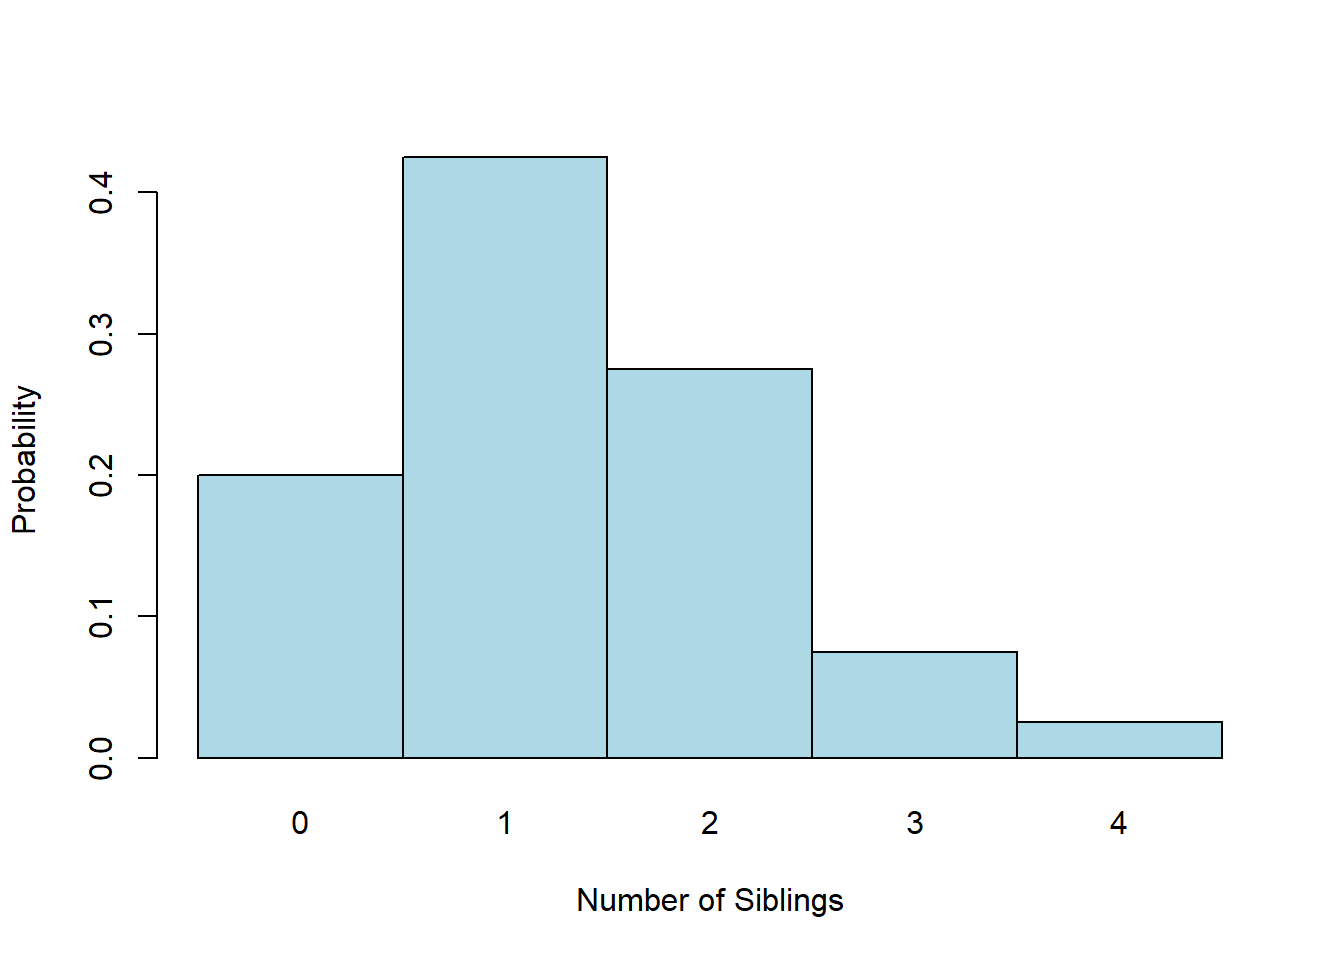
\includegraphics{IntroStats_files/figure-latex/unnamed-chunk-41-1.pdf}

The t-distribution is symmetric and always centered at 0. When \(n\ge30\), the t-distribution is approximately equivalent to the standard normal distribution. For smaller sample sizes, the t-distribution has more area in the tails (and therefore less area in the center of the distribution).

For a sample of size \(n < 30\), we plug in \(s\) for \(\sigma\) and use a t critical value (instead of a z critical value): \[\bar{x} \pm t_{df, \alpha/2}\frac{s}{\sqrt{n}}.\]

To find a t critical value, we will again use \texttt{R}, now with the command \texttt{qt(p,\ df)}. (Notice that this is similar to the command for the standard normal distribution, but instead of ``norm'' for normal it has ``t'' for the t-distribution.) For example, for a 98\% interval with a sample size of 15, \[100(1-\alpha) = 98 \implies \alpha=0.02\] Then \(\alpha/2 = 0.01\) and \(df=15-1=14\).

\begin{Shaded}
\begin{Highlighting}[]
\FunctionTok{qt}\NormalTok{(}\FloatTok{0.01}\NormalTok{, }\AttributeTok{df=}\DecValTok{14}\NormalTok{)}
\end{Highlighting}
\end{Shaded}

\begin{verbatim}
## [1] -2.624494
\end{verbatim}

which gives the t critical value \(t_{14,\alpha/2} = 2.624\). Notice again that I am able to ignore the sign because our formula uses \(\pm t_{df,\alpha/2}\).

As before, if you prefer you may use an applet, the Rossman and Chance t Probability Calculator instead of \texttt{R}.

\hypertarget{summary-of-confidence-interval-settings}{%
\section{Summary of Confidence Interval Settings}\label{summary-of-confidence-interval-settings}}

\textbf{Setting 1: \(\mu\) is target parameter, \(X\) is normal, \(\sigma\) known}

\begin{itemize}
\tightlist
\item
  Critical value: \(z_{\alpha/2}\)
\item
  Confidence interval: \[\bar{x} \pm z_{\alpha/2}\frac{\sigma}{\sqrt{n}}.\]
\end{itemize}

\textbf{Setting 2: \(\mu\) is target parameter, \(n \ge 30\), \(\sigma\) unknown}

\begin{itemize}
\tightlist
\item
  Critical value: \(z_{\alpha/2}\)
\item
  Confidence interval: \[\bar{x} \pm z_{\alpha/2}\frac{s}{\sqrt{n}}.\]
\end{itemize}

\textbf{Setting 3: \(\mu\) is target parameter, \(n < 30\), \(\sigma\) unknown}

\begin{itemize}
\tightlist
\item
  Critical value: \(t_{df, \alpha/2}\)
\item
  Confidence interval: \[\bar{x} \pm t_{df, \alpha/2}\frac{s}{\sqrt{n}}.\]
\end{itemize}

\hypertarget{introduction-to-hypothesis-testing}{%
\chapter{Introduction to Hypothesis Testing}\label{introduction-to-hypothesis-testing}}

\hypertarget{module-overview-5}{%
\section{Module Overview}\label{module-overview-5}}

In this module, we will continue our discussion on statistical inference with a discussion on hypothesis testing. In hypothesis testing, we take a more active approach to our data by asking questions about population parameters and developing a framework to answer those questions. We will root this discussion in confidence intervals before learning about several other approaches to hypothesis testing.

\textbf{Module Learning Outcomes/Objectives}

Test one sample means, paired data, and two sample means using confidence intervals and the critical or p-value approach.

This module's outcomes correspond to course outcomes (6) apply statistical inference techniques of parameter estimation such as point estimation and confidence interval estimation and (7) apply techniques of testing various statistical hypotheses concerning population parameters.

\hypertarget{logic-of-hypothesis-testing}{%
\section{Logic of Hypothesis Testing}\label{logic-of-hypothesis-testing}}

One of our goals with statisticial inference is to make decisions or judgements about the value of a parameter. A confidence interval is a good starting point, but we might also want to ask questions like

\begin{itemize}
\tightlist
\item
  Do cans of soda actually contain 12 oz?
\item
  Is Medicine A better than Medicine B?
\end{itemize}

A \textbf{hypothesis} is a statement that something is true. A hypothesis test involves two (competing) hypotheses:

\begin{enumerate}
\def\labelenumi{\arabic{enumi}.}
\tightlist
\item
  The \textbf{null hypothesis}, denoted \(H_0\), is the hypothesis to be tested. This is the ``default'' assumption.
\item
  The \textbf{alternative hypothesis}, denoted \(H_A\) is the alternative to the null.
\end{enumerate}

Note that the subscript 0 is ``nought'' (pronounced ``not''). A \textbf{hypothesis test} helps us decide whether the null hypothesis should be rejected in favor of the alternative.

\begin{quote}
\emph{Example}: Cans of soda are labeled with ``12 FL OZ''. Is this accurate?

The default, or uninteresting, assumption is that cans of soda contain 12 oz.

\begin{itemize}
\tightlist
\item
  \(H_0\): the mean volume of soda in a can is 12 oz.
\item
  \(H_A\): the mean volume of soda in a can is NOT 12 oz.
\end{itemize}
\end{quote}

We can write these hypotheses in words (as above) or in statistical notation. The null specifies a single value of \(\mu\):

\begin{itemize}
\tightlist
\item
  \(H_0\): \(\mu=\mu_0\)
\end{itemize}

We call \(\mu_0\) the \textbf{null value}. When we run a hypothesis test, \(\mu_0\) will be replaced by some number. For the soda can example, the null value is 12. We would write \(H_0: \mu = 12\).

The alternative specifies a \emph{range} of possible values for \(\mu\):

\begin{itemize}
\tightlist
\item
  \(H_A\): \(\mu\ne\mu_0\). ``The mean is different from the null value.''
\end{itemize}

\textbf{The Logic of Hypothesis Testing}

Take a random sample from the population. If the data area consistent with the null hypothesis, do not reject the null hypothesis. If the data are inconsistent with the null hypothesis \emph{and} supportive of the alternative hypothesis, reject the null in favor of the alternative.

\begin{quote}
\emph{Example}: One way to think about the logic of hypothesis testing is by comparing it to the U.S. court system. In a jury trial, jurors are told to assume the defendant is ``innocent until proven guilty''. Innocence is the default assumption, so

\begin{itemize}
\tightlist
\item
  \(H_0\): the defendant is innocent.
\item
  \(H_A\): the defendant is guilty.
\end{itemize}

Like in hypothesis testing, it is not the jury's job to decide if the defendant is innocent. That should be their default assumption. They are only there to decide if the defendant is guilty or if there is not enough evidence to override that default assumption. The \emph{burden of proof} lies on the alternative hypothesis.
\end{quote}

Notice the careful language in the logic of hypothesis testing: we either reject, or fail to reject, the null hypothesis. We never ``accept'' a null hypothesis.

\hypertarget{decision-errors}{%
\subsection{Decision Errors}\label{decision-errors}}

\begin{itemize}
\tightlist
\item
  A \textbf{Type I Error} is rejecting the null when it is true. (Null is true, but we conclude null is false.)
\item
  A \textbf{Type II Error} is not rejecting the null when it is false. (Null is false, but we do not conclude it is false.)
\end{itemize}

\(H_0\) is

True

False

Decision

Do not reject \(H_0\)

Correct decision

Type II Error

Reject \(H_0\)

Type I Error

Correct decision

\begin{quote}
\emph{Example}: In our jury trial,

\begin{itemize}
\tightlist
\item
  \(H_0\): the defendant is innocent.
\item
  \(H_A\): the defendant is guilty.
\end{itemize}

A Type I error is concluding guilt when the defendant is innocent. A Type II error is failing to convict when the person is guilty.
\end{quote}

How likely are we to make errors? Well, \(P(\)Type I Error\()=\alpha\), the \textbf{significance level}. (Yes, this is the same \(\alpha\) we saw in confidence intervals!) For Type II error, \(P(\)Type II Error\()=\beta\). This is related to the sample size calculation from the previous module, but is otherwise something we don't have time to cover.

We would like both \(\alpha\) and \(\beta\) to be small but, like many other things in statistics, there's a trade off! For a fixed sample size,

\begin{itemize}
\tightlist
\item
  If we decrease \(\alpha\), then \(\beta\) will increase.
\item
  If we increase \(\alpha\), then \(\beta\) will decrease.
\end{itemize}

In practice, we set \(\alpha\) (as we did in confidence intervals). We can improve \(\beta\) by increasing sample size. Since resources are finite (we can't get enormous sample sizes all the time), we will need to consider the consequences of each type of error.

\begin{quote}
\emph{Example} We could think about assessing consequences through the jury trial example. Consider two possible charges:

\begin{enumerate}
\def\labelenumi{\arabic{enumi}.}
\tightlist
\item
  Defendant is accused of stealing a loaf of bread. If found guilty, they may face some jail time and will have a criminal record.
\item
  Defendant is accused of murder. If found guilty, they will have a felony and may spend decades in prison.
\end{enumerate}

Since these are moral questions, I will let you consider the consequences of each type of error. However, keep in mind that we do make scientific decisions that have lasting impacts on people's lives.
\end{quote}

\textbf{Hypothesis Test Conclusions}

\begin{itemize}
\tightlist
\item
  If the null hypothesis is rejected, we say the result is \textbf{statistically significant}. We can interpret this result with:

  \begin{itemize}
  \tightlist
  \item
    At the \(\alpha\) level of significance, the data provide sufficient evidence to support the alternative hypothesis.
  \end{itemize}
\item
  If the null hypothesis is \emph{not} rejected, we say the result is \textbf{not statistically significant}. We can interpret this result with:

  \begin{itemize}
  \tightlist
  \item
    At the \(\alpha\) level of significance, the data do \emph{not} provide sufficient evidence to support the alternative hypothesis.
  \end{itemize}
\end{itemize}

Notice that these conclusions are framed in terms of the alternative hypothesis, which is either supported or not supported. We will \emph{never} conclude the null hypothesis. Finally, when we write these types of conclusions, we will write them in the context of the problem.

\hypertarget{confidence-interval-approach-to-hypothesis-testing}{%
\section{Confidence Interval Approach to Hypothesis Testing}\label{confidence-interval-approach-to-hypothesis-testing}}

We can use a confidence interval to help us weigh the evidence against the null hypothesis. A confidence interval gives us a range of \emph{plausible} values for \(\mu\). If the null value is in the interval, then \(\mu_0\) is a plausible value for \(\mu\). If the null value is \emph{not} in the interval, then \(\mu_0\) is \emph{not} a plausible value for \(\mu\).

\begin{enumerate}
\def\labelenumi{\arabic{enumi}.}
\tightlist
\item
  State null and alternative hypotheses.
\item
  Decide on significance level \(\alpha\). Check assumptions (decide which confidence interval setting to use).
\item
  Find the critical value.
\item
  Compute confidence interval.
\item
  If the null value is \emph{not} in the confidence interval, reject the null hypothesis. Otherwise, do not reject.
\item
  Interpret results in the context of the problem.
\end{enumerate}

\begin{quote}
\emph{Example}: Is the average mercury level in dolphin muslces different from \(2.5\mu g/g\)? Test at the 0.05 level of significance. A random sample of \(19\) dolphins resulted in a mean of \(4.4 \mu g/g\) and a standard deviation of \(2.3 \mu g/g\).

\begin{enumerate}
\def\labelenumi{\arabic{enumi}.}
\tightlist
\item
  \(H_0: \mu = 2.5\) and \(H_A: \mu \ne 2.5\).
\item
  Significance level is \(\alpha=0.05\). The value of \(\sigma\) is unknown and \(n = 19 < 30\), so we are in setting 3.
\item
  For setting 3, the critical value is \(t_{df, \alpha/2}\). Here, \(df=n-1=18\) and \(\alpha/2 = 0.025\):
\end{enumerate}
\end{quote}

\begin{Shaded}
\begin{Highlighting}[]
\FunctionTok{qt}\NormalTok{(}\FloatTok{0.025}\NormalTok{, }\DecValTok{18}\NormalTok{)}
\end{Highlighting}
\end{Shaded}

\begin{verbatim}
## [1] -2.100922
\end{verbatim}

\begin{quote}
\begin{enumerate}
\def\labelenumi{\arabic{enumi}.}
\setcounter{enumi}{3}
\tightlist
\item
  The confidence interval is \begin{align} \bar{x} &\pm t_{df, \alpha/2}\frac{s}{\sqrt{n}} \\ 4.4 &\pm 2.101 \frac{2.3}{\sqrt{19}} \\ 4.4 &\pm 1.109 \end{align} or \((3.29, 5.51)\).
\item
  Since the null value, \(2.5\), is not in the interval, it is \emph{not} a plausible value for \(\mu\) (at the 95\% level of confidence). Therefore we reject the null hypothesis.
\item
  At the 0.05 level of significance, the data provide sufficient evidence to conclude that the true mean mercury level in dolphin muscles is \emph{greater than} \(2.5\mu g/g\).
\end{enumerate}

Note: The alternative hypothesis is ``not equal to'', but we conclude ``greater than'' because all of the plausible values in the confidence interval are greater than the null value.
\end{quote}

\hypertarget{critical-value-approach-to-hypothesis-testing}{%
\section{Critical Value Approach to Hypothesis Testing}\label{critical-value-approach-to-hypothesis-testing}}

We learned about critical values when we discussed confidence intervals. Now, we want to use these values directly in a hypothesis test. We will compare these values to a value based on the data, called a \textbf{test statistic}.

Idea: the null is our ``default assumption''. If the null is true, how likely are we to observe a sample that looks like the one we have? If our sample is very inconsistent with the null hypothesis, we want to reject the null hypothesis.

\hypertarget{test-statistics}{%
\subsection{Test statistics}\label{test-statistics}}

Test statistics are similar to z- and t-scores: \[\text{test statistic} = \frac{\text{point estimate}-\text{null value}}{\text{standard error}}.\]

\begin{itemize}
\tightlist
\item
  \textbf{Setting 1}: \(\mu\) is target parameter, \(X\) is normal, \(\sigma\) known
\end{itemize}

\[z = \frac{\bar{x}-\mu_0}{\sigma/\sqrt{n}}\]

\begin{itemize}
\tightlist
\item
  \textbf{Setting 2}: \(\mu\) is target parameter, \(n \ge 30\), \(\sigma\) unknown
\end{itemize}

\[z = \frac{\bar{x}-\mu_0}{s/\sqrt{n}}\]

\begin{itemize}
\tightlist
\item
  \textbf{Setting 3}: \(\mu\) is target parameter, \(n < 30\), \(\sigma\) unknown
\end{itemize}

\[t = \frac{\bar{x}-\mu_0}{s/\sqrt{n}}\]

In fact, they serve a similar function in converting a variable \(\bar{X}\) into a distribution we can work with easily.

The set of values for the test statistic that cause us to reject \(H_0\) is the \textbf{rejection region}. The remaining values are the \textbf{nonrejection region}. The value that separates these is the critical value!

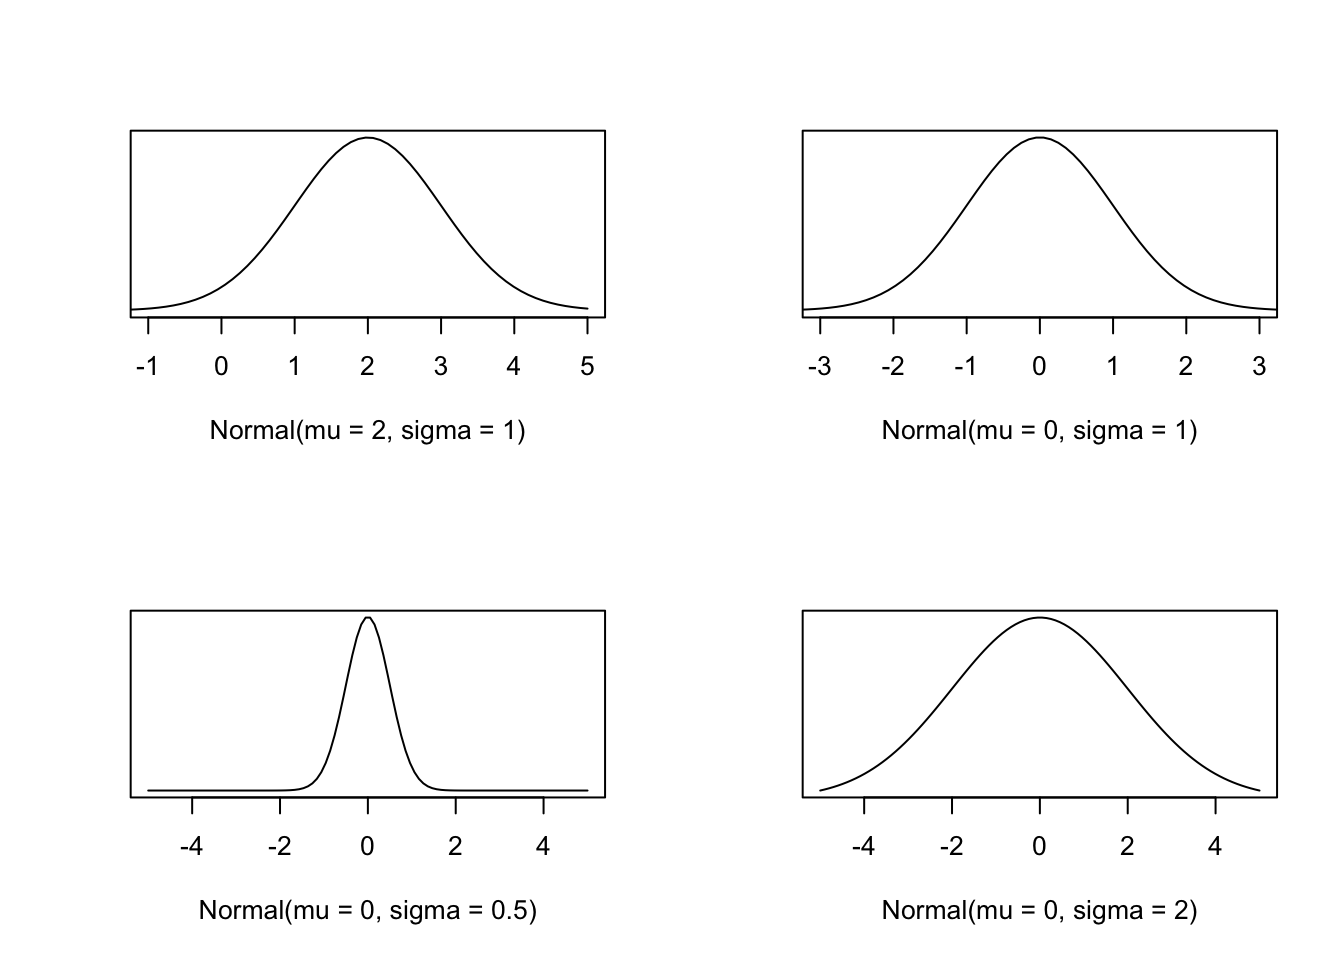
\includegraphics{IntroStats_files/figure-latex/unnamed-chunk-44-1.pdf}

Steps:

\begin{enumerate}
\def\labelenumi{\arabic{enumi}.}
\tightlist
\item
  State the null and alternative hypotheses.
\item
  Determine the significance level \(\alpha\). Check assumptions (decide which setting to use).
\item
  Compute the value of the test statistic.
\item
  Determine the critical values.
\item
  If the test statistic is in the rejection region, reject the null hypothesis. Otherwise, do not reject.
\item
  Interpret results.
\end{enumerate}

\begin{quote}
\emph{Example}: Is the average mercury level in dolphin muslces different from \(2.5\mu g/g\)? Test at the 0.05 level of significance. A random sample of \(19\) dolphins resulted in a mean of \(4.4 \mu g/g\) and a standard deviation of \(2.3 \mu g/g\).

\begin{enumerate}
\def\labelenumi{\arabic{enumi}.}
\tightlist
\item
  \(H_0: \mu = 2.5\) and \(H_A: \mu \ne 2.5\).
\item
  Significance level is \(\alpha=0.05\). The value of \(\sigma\) is unknown and \(n = 19 < 30\), so we are in setting 3.
\item
  The test statistic is \begin{align} t &= \frac{\bar{x}-\mu_0}{s/\sqrt{n}} \\ &= \frac{4.4-2.5}{2.3/\sqrt{19}} \\ &= 3.601 \end{align}
\item
  The critical value is \(t_{df, \alpha/2}\). Here, \(df=n-1=18\) and \(\alpha/2 = 0.025\):
\end{enumerate}
\end{quote}

\begin{Shaded}
\begin{Highlighting}[]
\FunctionTok{qt}\NormalTok{(}\FloatTok{0.025}\NormalTok{, }\DecValTok{18}\NormalTok{)}
\end{Highlighting}
\end{Shaded}

\begin{verbatim}
## [1] -2.100922
\end{verbatim}

\begin{quote}
\begin{enumerate}
\def\labelenumi{\arabic{enumi}.}
\setcounter{enumi}{4}
\tightlist
\item
  The test statistic is in the rejection region, so we will reject the null hypothesis:
\end{enumerate}
\end{quote}

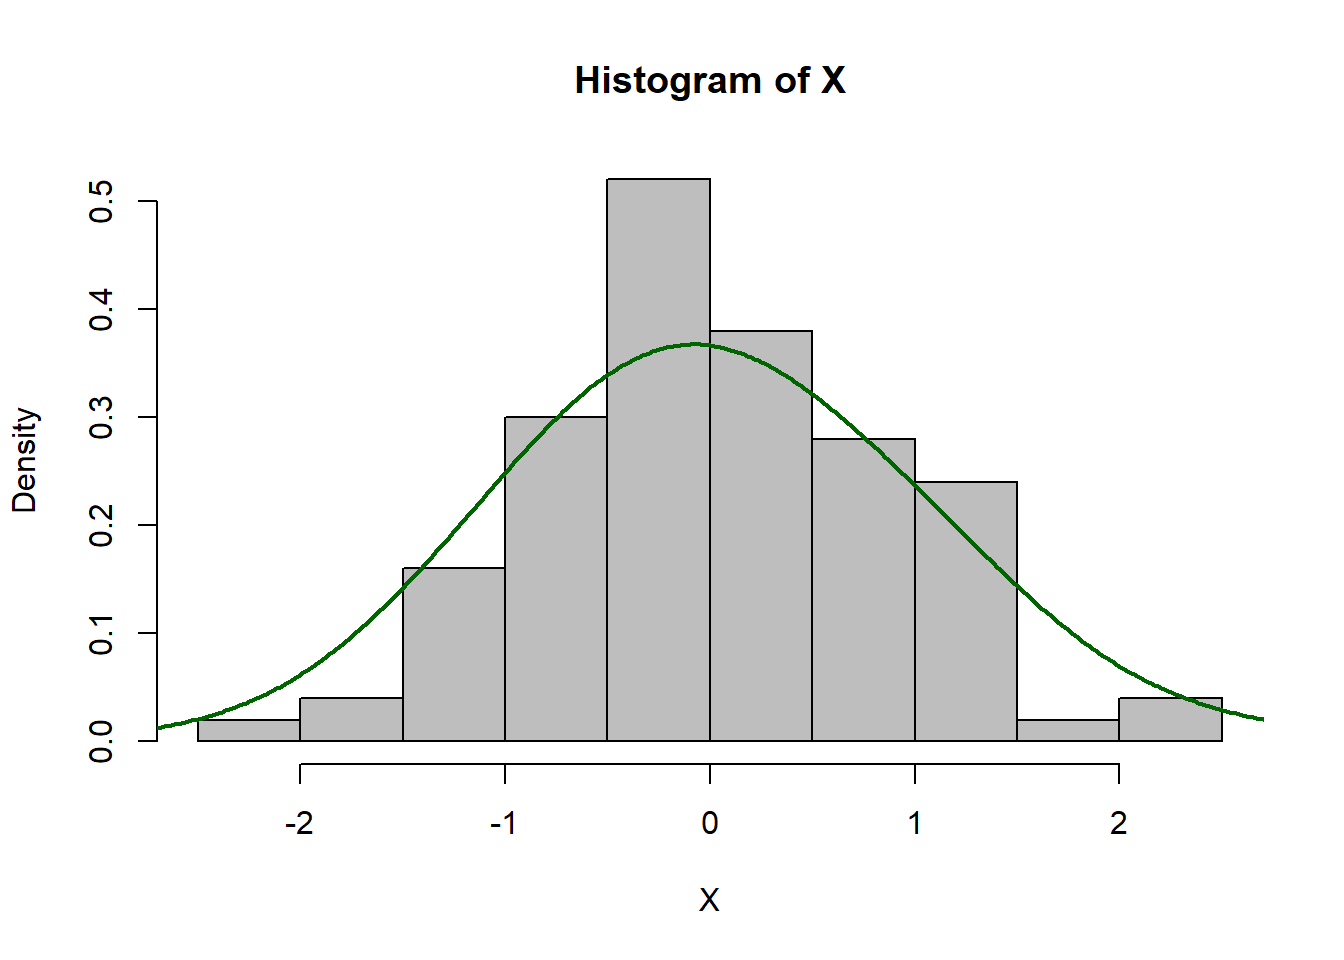
\includegraphics{IntroStats_files/figure-latex/unnamed-chunk-46-1.pdf}

\begin{quote}
\begin{enumerate}
\def\labelenumi{\arabic{enumi}.}
\setcounter{enumi}{5}
\tightlist
\item
  At the 0.05 level of significance, the data provide sufficient evidence to conclude that the true mean mercury level in dolphin muscles is greater than \(2.5\mu g/g\).
\end{enumerate}
\end{quote}

Notice that this is the same conclusion we came to when we used the confidence interval approach. These approaches are exactly equivalent!

\hypertarget{p-value-approach-to-hypothesis-testing}{%
\section{P-Value Approach to Hypothesis Testing}\label{p-value-approach-to-hypothesis-testing}}

If the null hypothesis is true, what is the probability of getting a random sample that is as inconsistent with the null hypothesis as the random sample we got? This probability is called the \textbf{p-value}?

\begin{quote}
\emph{Example}: Is the average mercury level in dolphin muslces different from \(2.5\mu g/g\)? Test at the 0.05 level of significance. A random sample of \(19\) dolphins resulted in a mean of \(4.4 \mu g/g\) and a standard deviation of \(2.3 \mu g/g\).

Probability of a sample \emph{as inconsistent} as our sample is \(P(t_{df} \text{ is as extreme as the test statistic})\). Consider \[P(t_{18} > 3.6) = 0.001\] but we want to think about the probability of being ``as extreme'' in \emph{either direction} (either tail), so \[\text{p-value} = 2P(t_{18}>3.6) = 0.002\]
\end{quote}

If \(\text{p-value} < \alpha\), reject the null hypothesis. Otherwise, do not reject.

\hypertarget{p-values}{%
\subsection{P-Values}\label{p-values}}

\begin{itemize}
\item
  \textbf{Setting 1}: \(\mu\) is target parameter, \(X\) is normal, \(\sigma\) known \[2P(Z > |z|)\] where \(z\) is the test statistic.
\item
  \textbf{Setting 2}: \(\mu\) is target parameter, \(n \ge 30\), \(\sigma\) unknown \[2P(Z > |z|)\] where \(z\) is the test statistic.
\item
  \textbf{Setting 3}: \(\mu\) is target parameter, \(n < 30\), \(\sigma\) unknown \[2P(t_{df} > |t|)\] where \(t\) is the test statistic.
\end{itemize}

Note: \(|a|\) is the ``absolute value'' of \(a\). The absolute value takes a number and throws away the sign, so \(|2|=2\) and \(|-3|=3\).

Steps:

\begin{enumerate}
\def\labelenumi{\arabic{enumi}.}
\tightlist
\item
  State the null and alternative hypotheses.
\item
  Determine the significance level \(\alpha\). Check assumptions (decide which setting to use).
\item
  Compute the value of the test statistic.
\item
  Determine the p-value.
\item
  If \(\text{p-value} < \alpha\), reject the null hypothesis. Otherwise, do not reject.
\item
  Interpret results.
\end{enumerate}

We often use p-values instead of the critical value approach because they are meaningful on their own (they have a direct interpretation).

\begin{quote}
\emph{Example}: For the dolphins,

\begin{enumerate}
\def\labelenumi{\arabic{enumi}.}
\tightlist
\item
  \(H_0: \mu = 2.5\) and \(H_A: \mu \ne 2.5\).
\item
  Significance level is \(\alpha=0.05\). The value of \(\sigma\) is unknown and \(n = 19 < 30\), so we are in setting 3.
\item
  The test statistic is \begin{align} t &= \frac{\bar{x}-\mu_0}{s/\sqrt{n}} \\ &= \frac{4.4-2.5}{2.3/\sqrt{19}} \\ &= 3.601 \end{align}
\item
  The p-value is \[2P(t_{df} > |t|) - 2P(t_{18} > 3.601) = 0.002\]
\item
  Since \(\text{p-value}=0.002 < \alpha=0.05\), reject the null hypothesis.
\item
  At the 0.05 level of significance, the data provide sufficient evidence to conclude that the true mean mercury level in dolphin muscles is greater than \(2.5\mu g/g\).
\end{enumerate}
\end{quote}

As before, this is the same conclusion we came to when we used the confidence interval and critical value approaches. All of these approaches are exactly equivalent.

\hypertarget{inference-beyond-the-mean}{%
\chapter{Inference: Beyond the Mean}\label{inference-beyond-the-mean}}

\hypertarget{module-overview-6}{%
\section{Module Overview}\label{module-overview-6}}

In this module, we extend the concepts from Module 6 to answer questions like ``is there a difference between these means?'' We will also consider hypothesis tests for whether a sample represents the population or closely matches a particular distribution.

\hypertarget{hypothesis-tests-for-two-means}{%
\section{Hypothesis Tests for Two Means}\label{hypothesis-tests-for-two-means}}

What if we wanted to \emph{compare} two means? We begin by discussing paired samples. This will feel very familiar, since it's essentially the same as hypothesis testing for a single mean. Then we will move on to independent samples, which will require a couple of adjustments.

\hypertarget{paired-samples}{%
\subsection{Paired Samples}\label{paired-samples}}

Sometimes there is a special correspondence between two sets of observations. We say that two sets of observations are \textbf{paired} if each observation has a natural connection with exactly one observation in the other data set. Consider the following data from 30 students given a pre- and post-test on a course concept:

\begin{longtable}[]{@{}ccc@{}}
\toprule
Student & Pre-Test & Post-Test \\
\midrule
\endhead
1 & 52 & 70 \\
2 & 71 & 98 \\
3 & 13 & 65 \\
\(\dots\) & \(\dots\) & \(\dots\) \\
30 & 48 & 81 \\
\bottomrule
\end{longtable}

The natural connection between ``pre-test'' and ``post-test'' is the student who took each test! Often, paired data will involve similar measures taken on the \emph{same item or individual}. We \emph{pair} these data because we want to compare two means, but we also want to account for the pairing.

Why? Consider: If a student got a 13\% on the pre-test, I would love to see them get a 60\% on the post-test - that's a huge improvement! But if a student got an 82\% on the pre-test, I would \emph{not} like to see them get a 60\% on the post-test. Pairing the data lets us account for this connection.

So what do we do with paired data? Fortunately, this part is easy! We start by taking the difference between the two sets of observations. In the pre- and post-test example, I will take the pre-test score and subtract the post-test score:

\begin{longtable}[]{@{}cccc@{}}
\toprule
Student & Pre-Test & Post-Test & \textbf{Difference} \\
\midrule
\endhead
1 & 52 & 70 & \textbf{18} \\
2 & 71 & 98 & \textbf{27} \\
3 & 13 & 65 & \textbf{52} \\
\(\dots\) & \(\dots\) & \(\dots\) & \(\dots\) \\
30 & 48 & 81 & \textbf{33} \\
\bottomrule
\end{longtable}

Then, we do a test of a \emph{single mean} on the differences where

\begin{itemize}
\tightlist
\item
  \(H_0: \mu_{\text{d}} = 0\)
\item
  \(H_A: \mu_{\text{d}} \ne 0\)
\end{itemize}

Note that the subscript ``d'' denotes ``difference''. We will use the exact same test(s) as in the previous sections:

\begin{itemize}
\item
  \textbf{Setting 1}: \(\mu_{\text{d}}\) is target parameter, the differences are approximately normal, \(\sigma_{\text{d}}\) known \[z = \frac{\bar{x}_{\text{d}}}{\sigma_{\text{d}}/\sqrt{n_{\text{d}}}}\] and the p-value is \[2P(Z > |z|)\] where \(z\) is the test statistic.
\item
  \textbf{Setting 2}: \(\mu_{\text{d}}\) is target parameter, \(n_{\text{d}} \ge 30\), \(\sigma_{\text{d}}\) unknown \[z = \frac{\bar{x}_{\text{d}}}{s_{\text{d}}/\sqrt{n_{\text{d}}}}\] and the p-value is \[2P(Z > |z|)\] where \(z\) is the test statistic.
\item
  \textbf{Setting 3}: \(\mu_{\text{d}}\) is target parameter, \(n_{\text{d}} < 30\), \(\sigma_{\text{d}}\) unknown \[t = \frac{\bar{x}_{\text{d}}}{s_{\text{d}}/\sqrt{n_{\text{d}}}}\] and the p-value is \[2P(t_{df} > |t|)\] where \(t\) is the test statistic.
\end{itemize}

Here, \(n_{\text{d}}\) is the number of pairs.

Steps:

\begin{enumerate}
\def\labelenumi{\arabic{enumi}.}
\tightlist
\item
  State the null and alternative hypotheses.
\item
  Determine the significance level \(\alpha\). Check assumptions (decide which setting to use).
\item
  Compute the value of the test statistic.
\item
  Determine the critical values or p-value.
\item
  For the \emph{critical value approach}: If the test statistic is in the rejection region, reject the null hypothesis. For the \emph{p-value approach}: If \(\text{p-value} < \alpha\), reject the null hypothesis. Otherwise, do not reject.
\item
  Interpret results.
\end{enumerate}

\hypertarget{independent-samples}{%
\subsection{Independent Samples}\label{independent-samples}}

In \textbf{independent samples}, the sample from one population does not impact the sample from the other population. In short, we take two \emph{separate samples} and compare them.

\begin{itemize}
\tightlist
\item
  \(H_0: \mu_1 = \mu_2 \quad \rightarrow \quad H_0: \mu_1 - \mu_2 = 0\)
\item
  \(H_A: \mu_1 \ne \mu_2 \quad \rightarrow \quad H_A: \mu_1 - \mu_2 \ne 0\)
\end{itemize}

If we use \(\bar{x}\) to estimate \(\mu\), intuitively we might use \(\bar{x}_1-\bar{x}_2\) to estimate \(\mu_1 - \mu_2\). To do this, we need to know something about the sampling distribution of \(\bar{x}_1-\bar{x}_2\).

Consider: if \(X_1\) is Normal(\(\mu_1\), \(\sigma_1\)) and \(X_2\) is Normal(\(\mu_2\),\(\sigma_2\)) with \(\sigma_1\) and \(\sigma_2\) are known, then for independent samples of size \(n_1\) and \(n_2\),

\begin{itemize}
\tightlist
\item
  \(\bar{X}_1-\bar{X}_2\) is Normal(\(\mu_{\bar{X}_1-\bar{X}_2}\), \(\sigma_{\bar{X}_1-\bar{X}_2}\)).
\item
  \(\mu_{\bar{X}_1-\bar{X}_2} = \mu_1 - \mu_2\)
\item
  \(\sigma_{\bar{X}_1-\bar{X}_2} = \sigma_1 - \sigma_2\)
\end{itemize}

so then \[Z = \frac{(\bar{X}_1 - \bar{X}_2) - (\mu_1 - \mu_2)}{\sqrt{\sigma_1/n_1 - \sigma_2/n_2}}\] has a standard normal distribution. But, as we mentioned earlier, we rarely work in that setting where the population standard deviation is known. Instead, we will use \(s_1\) and \(s_2\) to estimate \(\sigma_1\) and \(\sigma_2\). For independent samples of size \(n_1\) and \(n_2\), \[t = \frac{(\bar{X}_1 - \bar{X}_2) - (\mu_1 - \mu_2)}{\sqrt{s_1/n_1 - s_2/n_2}}\] has a t-distribution with degrees of freedom \[\Delta = \frac{[(s_1^2/n_1) + (s_2^2/n_2)]^2}{\frac{(s_1^2/n_1)^2}{n_1-1} + \frac{(s_2^2/n_2)^2}{n_2-1}}\] rounded \emph{down} to the nearest whole number.

\textbf{The Two-Sample T-Test}

Assumptions:

\begin{itemize}
\tightlist
\item
  Simple random samples.
\item
  Independent samples.
\item
  Normal populations or large (\(n \ge 30\)) samples.
\end{itemize}

\textbf{Steps for Critical Value Approach}:

\begin{enumerate}
\def\labelenumi{\arabic{enumi}.}
\tightlist
\item
  \(H_0: \mu_1 - \mu_2 = 0\) and \(H_A: \mu_1 - \mu_2 \ne 0\)
\item
  Check assumptions; select the significance level \(\alpha\).
\item
  Compute the test statistic \[t = \frac{\bar{x}_1 - \bar{x}_2}{\sqrt{s_1/n_1 - s_2/n_2}}\] Note that we assume under the null hypothesis that \(\mu_1 - \mu_2 = 0\), which is why we replace this quantity with \(0\) in the test statistic.
\item
  The critical value is \(\pm t_{df, \alpha/2}\) with \(df = \Delta\).
\item
  If the test statistic falls in the rejection region, reject the null hypothesis.
\item
  Interpret in the context of the problem.
\end{enumerate}

\textbf{Steps for P-Value Approach}:

\begin{enumerate}
\def\labelenumi{\arabic{enumi}.}
\tightlist
\item
  \(H_0: \mu_1 - \mu_2 = 0\) and \(H_A: \mu_1 - \mu_2 \ne 0\)
\item
  Check assumptions; select the significance level \(\alpha\).
\item
  Compute the test statistic \[t = \frac{\bar{x}_1 - \bar{x}_2}{\sqrt{s_1/n_1 - s_2/n_2}}\] Note that we assume under the null hypothesis that \(\mu_1 - \mu_2 = 0\), which is why we replace this quantity with \(0\) in the test statistic.
\item
  The p-value is \(2P(t_{df} > |t|)\) with \(df = \Delta\).
\item
  If \(\text{p-value}<\alpha\), reject the null hypothesis.
\item
  Interpret in the context of the problem.
\end{enumerate}

Notice that the only difference between the critical value and p-value approaches are steps 4 and 5.

\begin{quote}
\emph{Example}: Researchers wanted to detemine whether a dymanic or static approach would impact the time needed to complete neurosurgeries. The experiment resulted in the following data from simple random samples of patients:

\begin{longtable}[]{@{}cc@{}}
\toprule
Dynamic & Static \\
\midrule
\endhead
\(\bar{x}_1 = 394.6\) & \(\bar{x}_2 = 468.3\) \\
\(s_1 = 84.7\) & \(s_2 = 38.2\) \\
\(n_1 = 14\) & \(n_2 = 6\) \\
\bottomrule
\end{longtable}

Times are measured in minutes. Assume \(X_1\) and \(X_2\) are reasonably normal.

\begin{enumerate}
\def\labelenumi{\arabic{enumi}.}
\tightlist
\item
  \(H_0: \mu_1 = \mu_2\) and \(H_A: \mu_1\ne\mu_2\)
\item
  Let \(\alpha=0.05\) (this will be our default when a significance level is not given)

  \begin{itemize}
  \tightlist
  \item
    We are told these are simple random samples.
  \item
    There's no reason that time for a neurosurgery with the dynamic system would impact time for the static system (or vice versa), so it's reasonable to assume these samples are independent.
  \item
    We are told to assume that \(X_1\) and \(X_2\) are reasonably normal.
  \end{itemize}
\item
  The test statistic is \[t = \frac{394.6-468.3}{84.7^2/14 + 38.2^2/6} = -2.681\]
\item
  Then \[df = \Delta = \frac{(84.7^2/14) + (38.2^2/6)^2}{\frac{(84.7^2/14)^2}{14-1} + \frac{(38.2^2/6)^2}{6-1}} = 17\] when rounded down. The critical value is \[t_{17, 0.025} = 2.110\] and the p-value is \[2P(t_{17}>|-2.681|)=2(0.0079)=0.0158\]
\item
  For the critical value approach,
\end{enumerate}
\end{quote}

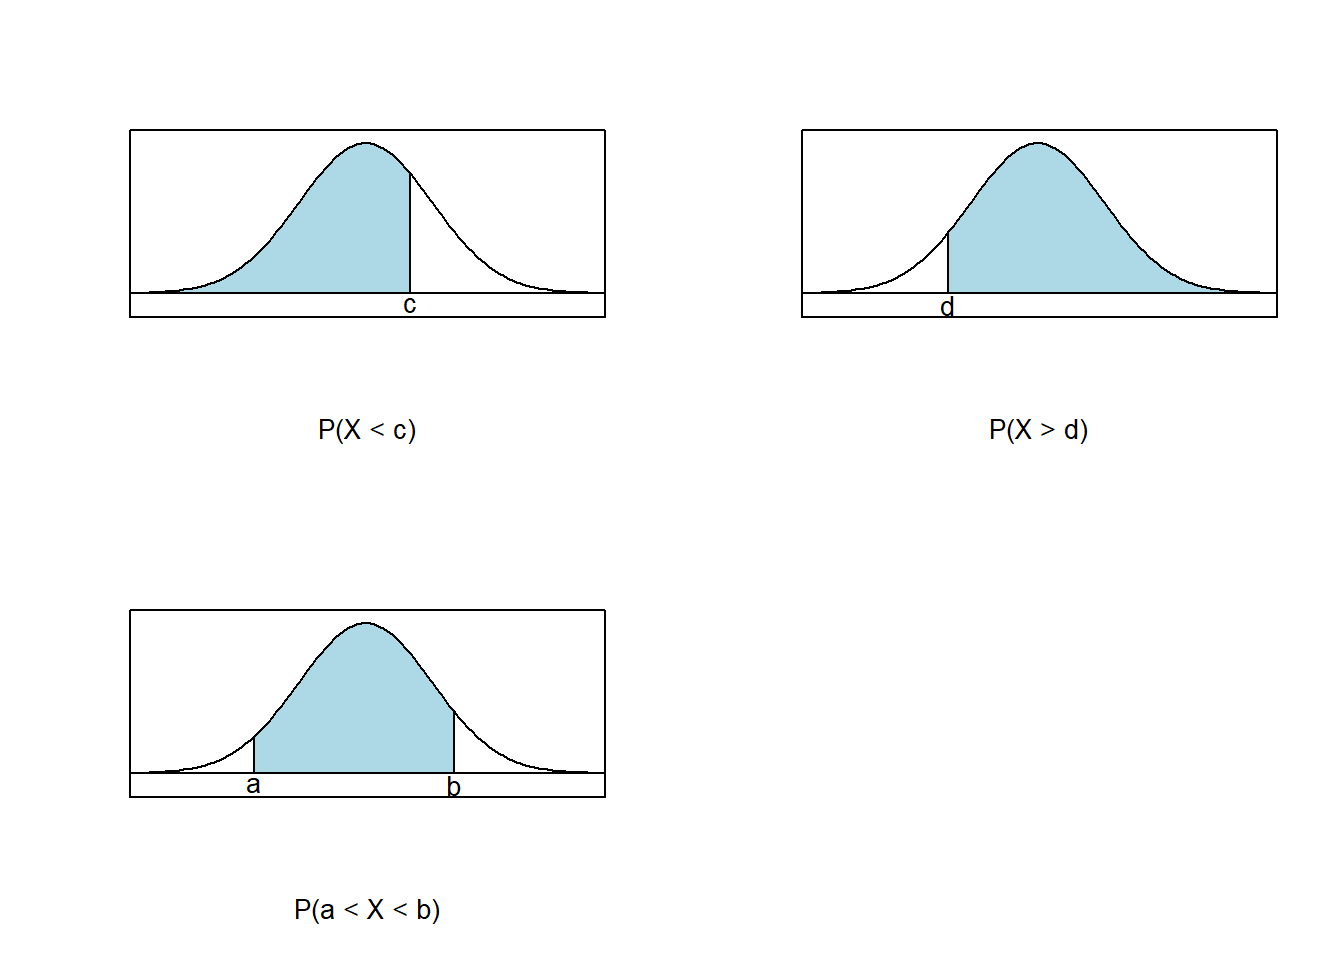
\includegraphics{IntroStats_files/figure-latex/unnamed-chunk-47-1.pdf}

\begin{quote}
Since the test statistic is in the rejection region, we reject the null hypothesis. For the p-value approach, since \(\text{p-value}=0.158 < \alpha =0.05\), reject the null hypothesis.

\begin{enumerate}
\def\labelenumi{\arabic{enumi}.}
\setcounter{enumi}{5}
\tightlist
\item
  At the 0.05 level of significance, the data provide sufficient evidence to conclude that the mean time for the dynamic system is less than the mean time for the static system.
\end{enumerate}
\end{quote}

We can also construct a \textbf{\((1-\alpha)100\%\) confidence interval} for the difference of the two population means: \[(\bar{x}_1-\bar{x}_2) \pm t_{df, \alpha/2}\sqrt{\frac{s_1^2}{n_1} + \frac{s_2^2}{n_2}}\] which we interpret as we interpret other confidence intervals, including in our interpretation that we are now considering the *difference of two means**.

\hypertarget{analysis-of-variance-anova}{%
\section{Analysis of Variance (ANOVA)}\label{analysis-of-variance-anova}}

Now that we've examined tests for one and two means, it's natural to wonder about three or more means. For example, we might want to compare three different medications: treatment 1 (\(t_1\)), treatment 2 (\(t_2\)), and treatment 3 (\(t_3\)). Based on what we've learned so far, we might think to do pairwise comparisons, examining \(t_1\) vs \(t_2\), then \(t_2\) vs \(t_3\), then \(t_1\) vs \(t_3\). Unfortunately, this tends to increase our Type I error!

Think of it this way: if I set my confidence level to 95\%, I'm setting my Type I error rate to \(\alpha=0.05\). In general terms, this means that about 1 out of every 20 times I run my experiment, I would make a type I error. If I went ahead and ran, say, 20 tests comparing two means, my \emph{overall} Type I error rate is going to increase - there's a pretty significant chance that at least one of those comparisons will results in a Type I error!

Instead, we will use a test that allows us to ask: ``Are all these means the same?'' This is called the \textbf{an}alysis \textbf{o}f \textbf{va}riance, or ANOVA.

\begin{itemize}
\tightlist
\item
  \(H_0\): The mean outcome is the same across all groups.
\item
  \(H_A\): At least one mean differs from the rest.
\end{itemize}

In statistical notation, these hypotheses look like:

\begin{itemize}
\tightlist
\item
  \(H_0: \mu_1 = \mu_2 = \dots = \mu_k\)
\item
  \(H_A: \mu_i \ne \mu_j\) for at least one pair \((i, j)\)
\end{itemize}

where \(k\) is the number of means being compared and the notation \(\mu_i\) represents the mean for the \(i\)th group (\(i\) can take on any whole number value between 1 and \(k\)).

For ANOVA, we have three key conditions:

\begin{enumerate}
\def\labelenumi{\arabic{enumi}.}
\tightlist
\item
  Observations are independent within and across groups.
\end{enumerate}

Independence within groups is the way we've been thinking about independence already. We want to convince ourselves that for any particular group, the observations do not impact each other. For independence across groups, we want to convince ourselves that the groups do not impact each other. Note: if we have a simple random sample, this assumption is always satisfied.

\begin{enumerate}
\def\labelenumi{\arabic{enumi}.}
\setcounter{enumi}{1}
\tightlist
\item
  Data within each group are approximately normal.
\end{enumerate}

If you make a histogram of the data for each group, each histogram will look approximately bell-shaped.

\begin{enumerate}
\def\labelenumi{\arabic{enumi}.}
\setcounter{enumi}{2}
\tightlist
\item
  Variability is approximately equal across groups.
\end{enumerate}

Take the standard deviation for each group and check if they are approximately equal. A boxplot is an appropriate way to do this visually.

\textbf{Why Variance?}

You may have seen the name ``analysis of variance'' and wondered what the variance has to do with comparing many means. Consider the following boxplots:

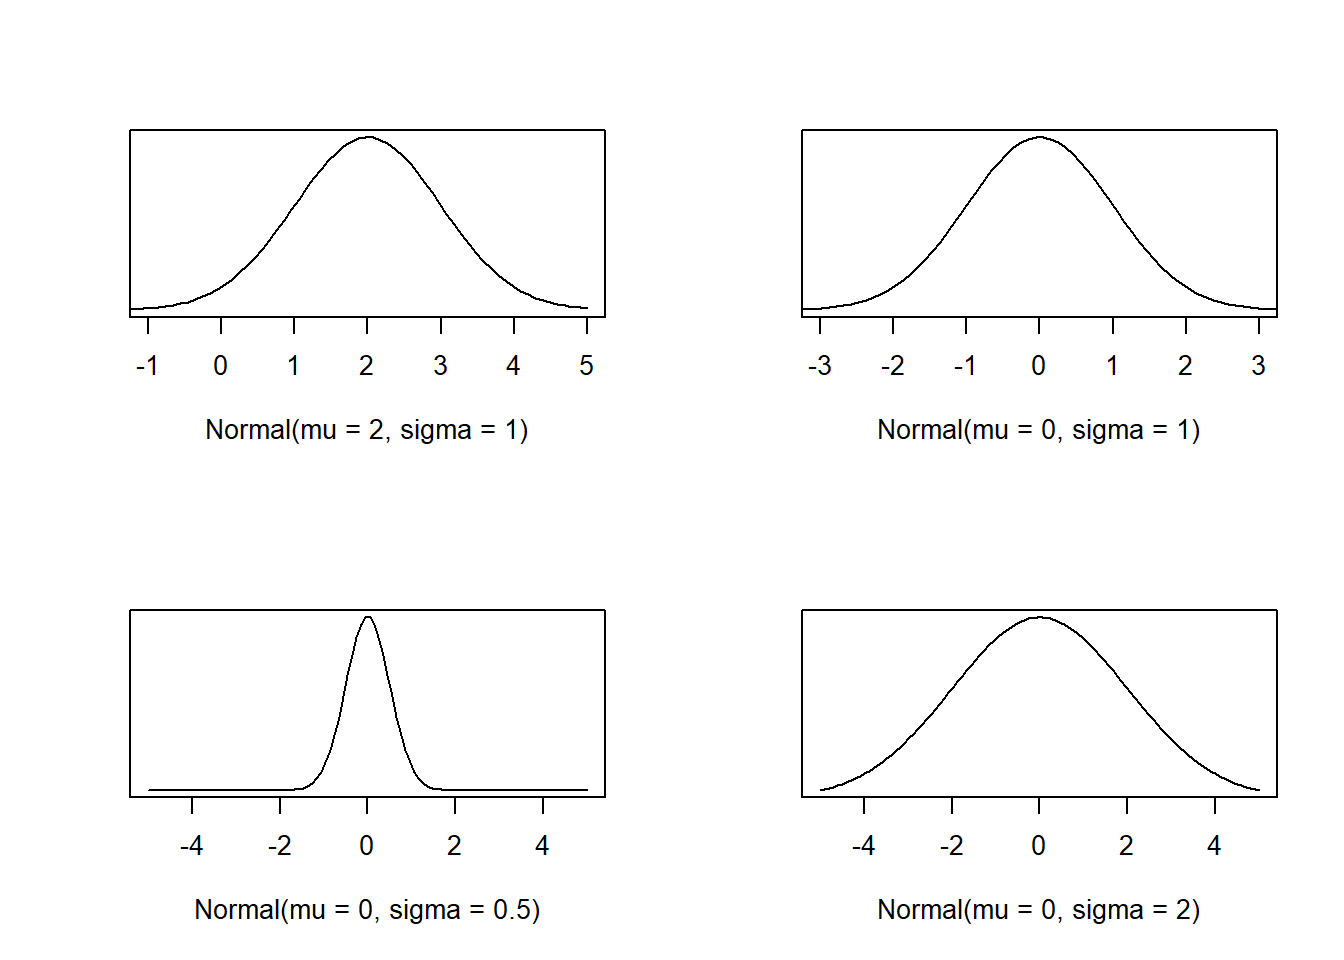
\includegraphics{IntroStats_files/figure-latex/unnamed-chunk-48-1.pdf}

Is there a difference in the means for Experiment 1? What about Experiment 2?

In fact, the means are \(\mu_1 = \mu_4 = 2\), \(\mu_2 = \mu_5 = 1\), and \(\mu_3 = \mu_6 = 0.5\). But the variances for the Experiment 1 groups are much larger than for the Experiment 2 groups! The larger variances in Experiment 1 obscure any differences between the group means. It is for this reason that we analyze variance as part of our test for differences in means.

\begin{quote}
Aside: Why can't we look at the data first and just test the two means that have the largest difference?

When we look at the data \emph{and then choose a test}, this inflates our Type I error rate! It's bad practice and not something we want to engage in as scientists.
\end{quote}

In order to perform an ANOVA, we need to consider whether the sample means differ more than we would expect them to based on natural variation (remember that we expect random samples to produce slightly different sample statistics each time!). This type of variation is called \textbf{mean square between groups} or \(MSG\). It has associated degrees of freedom \(df_G = k-1\) where \(k\) is the number of groups. Note that \[MSG = \frac{SSG}{df_G}\] where \(SSE\) is the \textbf{sum of squares group}. If the null hypothesis is true, variation in the sample means is due to chance. In this case, we would expect the MSG to be relatively small.

When I say ``relatively small'', I mean we need to compare this quantity to something. We need some quantity that will give us an idea of how much variability to expect if the null hypothesis is true. This is the \textbf{mean square error} or \(MSE\), which has degrees of freedom \(df_E = n-k\). Again, we have the relationship that \[MSE = \frac{SSE}{df_E}\] where \(SSE\) is the \textbf{sum of squares error}. These calculations are very similar to the calculation for variance (and standard deviation)! (Note: we will not calculate these quantities by hand, but if you are interested in the mathematical details they are available in the OpenIntro Statistics textbook in the footnote on page 289.)

We compare these two quantities by examining their ratio: \[F = \frac{MSG}{MSE}\] This is the test statistic for the ANOVA.

\hypertarget{the-f-distribution}{%
\subsection{The F-Distribution}\label{the-f-distribution}}

The \(\boldsymbol{F}\)\textbf{-test} relies on something called the \(F\) distribution. The \(F\) distribution has two parameters: \(df_1=df_G\) and \(df_1=df_E\). The \(F\) distribution always takes on positive values, so an \emph{extreme} or \emph{unusual} value for the \(F\) distribution will correspond to a large (positive) number.

When we run an ANOVA, we almost always use the p-value approach. If you are using \texttt{R} for your distributions, the command is \texttt{pf(F,\ df1,\ df2,\ lower.tail=FALSE)} where \texttt{F} is the test statistic.

\begin{quote}
\emph{Example:} Suppose I have a test with 100 observations and 5 groups. I find \(MSG = 0.041\) and \(MSE = 0.023\). Then \[df_G = k-1 = 5-1 = 4\] and \[df_E = n-k = 100-5 = 95\] The test statistic is \[f = \frac{0.041}{0.023} = 1.7826\] To find the p-value using \texttt{R}, I would write the command
\end{quote}

\begin{Shaded}
\begin{Highlighting}[]
\FunctionTok{pf}\NormalTok{(}\FloatTok{1.7826}\NormalTok{, }\DecValTok{4}\NormalTok{, }\DecValTok{95}\NormalTok{, }\AttributeTok{lower.tail=}\ConstantTok{FALSE}\NormalTok{)}
\end{Highlighting}
\end{Shaded}

\begin{verbatim}
## [1] 0.1387132
\end{verbatim}

\begin{quote}
and find a p-value of 0.1387.
\end{quote}

Here is a nice F-distribution applet. For this applet, \(\nu_1 = df_1\) and \(\nu_2 = df_2\). Plug in your \(F\) test statistic where it indicates ``x ='' and your p=value will appear in the red box next to ``P(X\textgreater x)''. When you enter your degrees of freedom, a visualization will appear similar to those in the Rossman and Chance applets we used previously.

\textbf{The ANOVA Table}

Generally, when we run an ANOVA, we create an ANOVA table (or we have software create one for us!). This table looks something like this

\begin{longtable}[]{@{}llllll@{}}
\toprule
& df & Sum of Squares & Mean Squares & F Value & P-Value \\
\midrule
\endhead
group & \(df_G\) & \(SSG\) & \(MSG\) & \(F\) & p-value \\
error & \(df_E\) & \(SSE\) & \(MSE\) & & \\
\bottomrule
\end{longtable}

\begin{quote}
\emph{Example:} chick weights

\texttt{R} has data on the weights of chicks fed six different feeds (diets). Assume these data are based on a random sample of chicks. There are \(n=71\) total observations and \(k=6\) different feeds. Let's assume we want to test with a 0.05 level of significance.

The ANOVA hypotheses are

\begin{itemize}
\tightlist
\item
  \(H_0\): the mean weight is the same for all six feeds.
\item
  \(H_A\): at least one feed has a mean weight that differs.
\end{itemize}

The summaries for these data are
\end{quote}

\begin{verbatim}
##         casein horsebean linseed meatmeal soybean sunflower
## n        12.00     10.00   12.00    11.00   14.00     12.00
## Mean    323.58    160.20  218.75   276.91  246.43    328.92
## Std Dev  64.43     38.63   52.24    64.90   54.13     48.84
\end{verbatim}

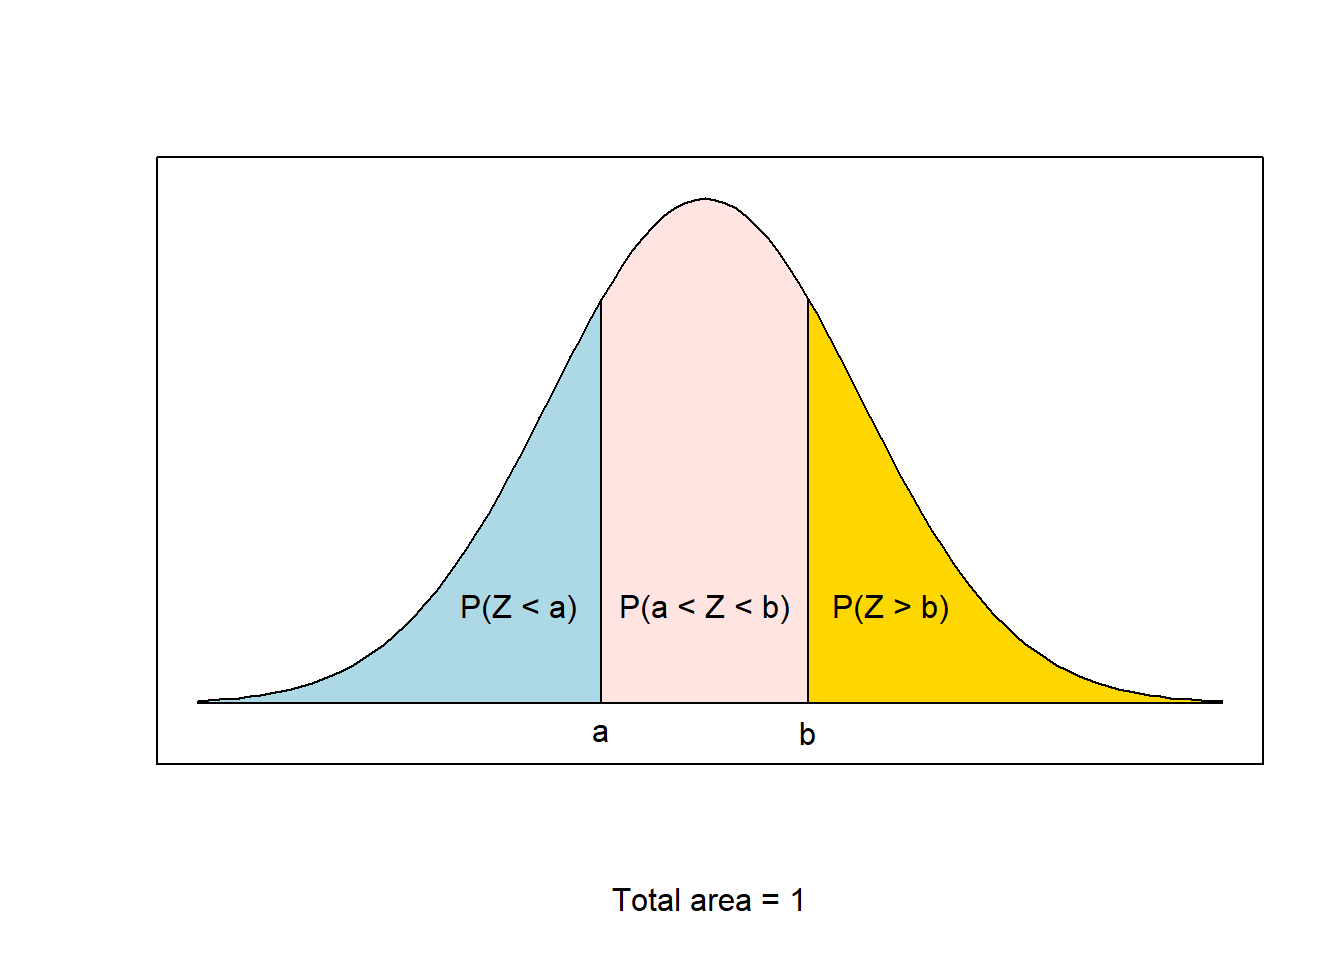
\includegraphics{IntroStats_files/figure-latex/unnamed-chunk-50-1.pdf} 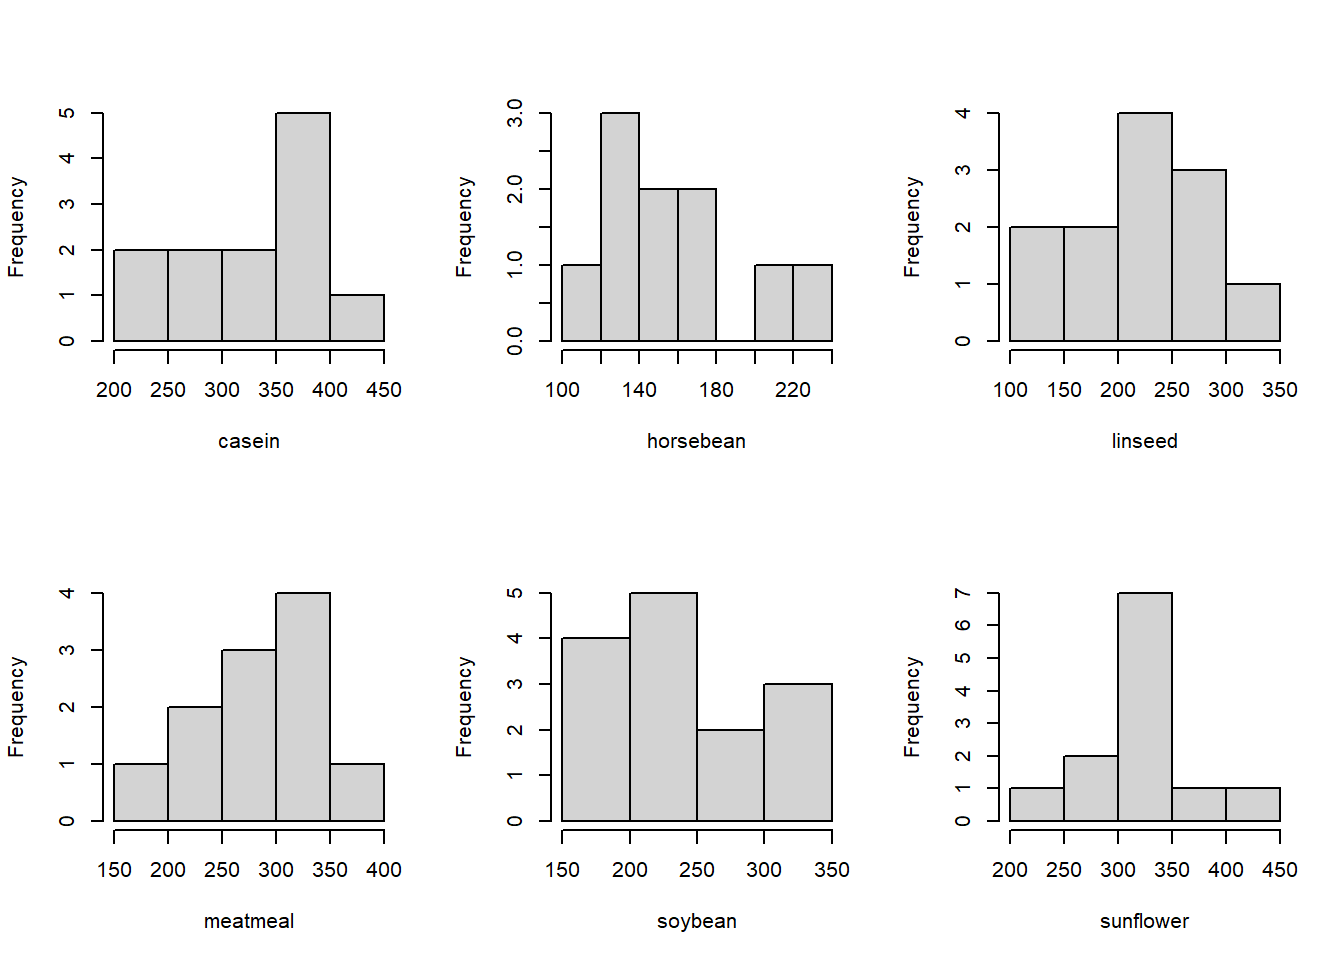
\includegraphics{IntroStats_files/figure-latex/unnamed-chunk-50-2.pdf}

\begin{quote}
The group sizes are relatively small, so it's difficult to determine how far from normality these data are based on the histograms. We may also run into some issues with constant variance. However, for the sake of the example, let's push ahead with the ANOVA! Since we usually use software to calculate ANOVAs, I've used \texttt{R} to create the following ANOVA table:
\end{quote}

\begin{verbatim}
## Analysis of Variance Table
## 
## Response: chickwts$weight
##               Df Sum Sq Mean Sq F value    Pr(>F)    
## chickwts$feed  5 231129   46226  15.365 5.936e-10 ***
## Residuals     65 195556    3009                      
## ---
## Signif. codes:  0 '***' 0.001 '**' 0.01 '*' 0.05 '.' 0.1 ' ' 1
\end{verbatim}

\begin{quote}
From the table, we can confirm that \(df_G = 6-1 = 5\) and \(df_E = 71 - 6 = 65\). The F test statistic is \[MSG/MSE = 46226 / 3009 = 15.365\] Finally, the p-value is \(5.936\times10^{-10}\). Clearly \(5.936\times10^{-10} < \alpha = 0.05\), so we will reject the null hypothesis and conclude that at least one of the feed groups has a mean weight that differs.
\end{quote}

\hypertarget{multiple-comparisons-and-type-i-error-rate}{%
\subsection{Multiple Comparisons and Type I Error Rate}\label{multiple-comparisons-and-type-i-error-rate}}

Let's return for a moment to our ANOVA hypotheses:

\begin{itemize}
\tightlist
\item
  \(H_0\): The mean outcome is the same across all groups.
\item
  \(H_A\): At least one mean differs from the rest.
\end{itemize}

If we reject \(H_0\) and conclude that ``at least one mean differs from the rest'', how do we determine which mean(s) differ? \emph{If} we reject \(H_0\), we will perform a series of two-sample t-tests. But wait! What about the Type I error? Isn't this exactly what we decided we couldn't do when we introduced ANOVA?

In order to avoid this increased Type I error rate, we run these \textbf{mulitple comparisons} with a modified significance level. There are several ways to do this, but the most common way is with the \textbf{Bonferroni correction}. Here, if we want to test at the \(100(1-\alpha)\) level of significance, we run each of our pairwise comparisons with \[\alpha^* = \alpha/K\] where \(K\) is the number of comparisons being considered. For \(k\) groups, there are \[K = \frac{k(k-1)}{2}\] possible pairwise comparisons.

For these comparisons, we use a special pooled estimate of the standard deviation, \(s_{\text{pooled}}\) in place of \(s_1\) and \(s_2\): \[\text{standard error} = \sqrt{\frac{s_{\text{pooled}}^2}{n_1} + \frac{s_{\text{pooled}}^2}{n_2}}\] Other than changing \(\alpha\) to \(\alpha^*\) and the standard error to this new formula, the test is exactly the same as that discussed in the previous section. Note that \[s_{\text{pooled}} = \sqrt{MSE}\] and the degrees of freedom is \(df_E\).

\begin{quote}
\emph{Example}: chick weights

Let's extend our discussion on the chick weights to multiple comparisons. Since we were able to conclude that at least one feed has a weight that differs, we want to find out where the difference(s) lie!

We will test all possible pairwise comparisons. This will require \(K = \frac{6(6-1)}{2} = 15\) tests. The pooled standard deviation is \(s_{pooled} = \sqrt{3009} \approx 54.85\). Let's walk through the test of casein \((\bar{x}_1 = 323.58, n=12)\) vs horsebean \((\bar{x}_2 = 160.20, n=10)\):

\begin{itemize}
\tightlist
\item
  \(H_0: \mu_1 = \mu_2\)
\item
  \(H_A: \mu_1 \ne \mu_2\)
\end{itemize}

The estimated difference and standard error are \[\bar{x}_1 - \bar{x}_2 = 323.58 - 160.20 = 163.38 \quad\quad SE = \sqrt{\frac{54.85^2}{11}+\frac{54.85^2}{9}} = 25.65\] which results in a test statistic of \(t=6.37\) and a p-value of \(1.11\times10^{-8}\). We then compare this to \(\alpha^* = 0.05/15 = 0.0033\). Since the p-value of \(1.11\times10^{-8} < \alpha^* = 0.0033\), we reject the null hypothesis and conclude there is a significant difference in mean chick weight between the casein and horsebean feeds.

In order to complete the pairwise comparisons, we would then run the remaining 14 tests. I will leave this as an optional exercise for the particularly motivated student.
\end{quote}

Note: occasionally, we may reject \(H_0\) in the ANOVA but may fail to find any statistically significant differences when performing multiple comparisons with the Bonferroni correction. This is ok! It just means we were unable to identify which specific groups differ.

  \bibliography{book.bib,packages.bib}

\end{document}
